\documentclass[10pt,letterpaper]{article}
\usepackage{multicol}
\usepackage{multirow}
\usepackage{longtable}
\usepackage{graphicx} % Required for inserting images
\usepackage{tikz}
\usepackage[margin=0.75in]{geometry}
\usepackage{courier} % Required to support bold monospace
\usepackage{pgf}
\usepackage{amsmath}
\usepackage{amsfonts}
\usepackage{listings}
\usepackage{tabularx}
\usepackage{makecell}
\usepackage{adjustbox}
\usepackage[justification=centering]{caption}
\usetikzlibrary{positioning,calc,arrows,arrows.meta,automata,shapes}
\usepackage{titlesec}
\usepackage{CJKutf8}
\usepackage{microtype}
\usepackage[ruled,vlined]{algorithm2e}
% hyperref LAST
\usepackage[unicode,hidelinks]{hyperref}

\titleformat{\section}[hang]
  {\normalfont\Large\bfseries\raggedright}
  {\thesection}
  {1em}
  {}

\titleformat{\subsection}[hang]
  {\normalfont\large\bfseries\raggedright}
  {\thesubsection}
  {1em}
  {}

\lstdefinestyle{customc}{
  language=C,
  breaklines=true,
  breakatwhitespace=false,  % Usually better for C code
  numbers=none,
  numberstyle=\tiny,
  basicstyle=\ttfamily\footnotesize,
  keywordstyle=\color{blue},
  commentstyle=\color{gray}\itshape,
  showstringspaces=false,
  tabsize=4,
  frame=single,
  columns=flexible,
  escapeinside={(*@}{@*)}
}
\lstdefinestyle{custompy}{
  language=Python,
  breaklines=true,
  breakatwhitespace=false,  % Usually better for C code
  numbers=none,
  numberstyle=\tiny,
  basicstyle=\ttfamily\footnotesize,
  keywordstyle=\color{blue},
  commentstyle=\color{gray}\itshape,
  showstringspaces=false,
  tabsize=4,
  frame=single,
  columns=flexible,
  escapeinside={(*@}{@*)}
}

\title{``BREAKMEIFYOUCAN!'': Exploiting Keyspace Reduction and Relay Attacks in 3DES and AES-protected NFC Technologies}
\author{Nathan Nye, Philippe Teuwen, Tiernan Messmer,\\
        Steven Mauch, Struan Clark, Zinong Li, Zachary Weiss, Lucifer Voeltner}
\date{\today~--- Rev. 1}

\hypersetup{
  pdftitle={BREAKMEIFYOUCAN!: Exploiting Keyspace Reduction and Relay Attacks in 3DES and AES-protected NFC Technologies},
  pdfauthor={Nathan Nye; Philippe Teuwen; Tiernan Messmer; Steven Mauch; Struan Clark; Zinong Li; Zachary Weiss; Lucifer Voeltner},
  pdfsubject={NFC security, cryptanalysis, relay attacks, partial key overwrite attacks, EEPROM tearing attacks},
  pdfkeywords={NFC, contactless, MIFARE, 3DES, AES, relay attack, partial key overwrite, PKO, keyspace reduction, Ultralight, NTAG, security research},
  pdfcreator={LaTeX with pdflatex},
  pdfproducer={pdfTeX},
  pdfstartview=FitH,
  pdfpagemode=UseNone
}

\hyphenpenalty=10000
\begin{document}

\maketitle
\begin{center}
\texttt{firstname.lastname@breakmeifyoucan.com}
\end{center}

\begin{abstract}
This paper presents an in-depth analysis of vulnerabilities in MIFARE Ultralight~C (MF0ICU2), MIFARE Ultralight~AES (MF0AES), NTAG~223~DNA (NT2H2331G0 and NT2H2331S0), NTAG~224~DNA (NT2H2421G0 and NT2H2421S0), and widely circulated counterfeit Ultralight~C cards based on Giantec GT23SC4489, Feiju FJ8010, and USCUID-UL. We reveal multiple avenues to substantially weaken the security of each technology and its implementation across a range of configurations. We demonstrate how, through relay-based man-in-the-middle techniques and partial key overwrites --- optionally combined with tearing techniques --- an attacker can reduce the keyspace of two-key Triple DES (2TDEA) from $2^{112}$ to $2^{28}$ or less in certain real-world deployments, thereby making brute-force key recovery feasible with modest computational resources. We further discuss how the MIFARE Ultralight~AES protocol can be similarly affected, particularly when CMAC integrity checks are not enforced. We also find that the security offered by NTAG~223~DNA and NTAG~224~DNA is undermined by the absence of integrity checks on commands and the calculation of a CMAC over Secure Unique NFC (SUN) messages, providing an unauthenticated ciphertext oracle that facilitates key recovery. Field observations, especially in hospitality deployments, underscore the urgent need for proper configuration, key diversification, and counterfeit detection.
\end{abstract}

\begin{multicols}{2}
\section{Introduction}
Low cost contactless tags have become a ubiquitous component in contemporary large-scale deployments such as transport ticketing, hospitality access, and event management. Among these, the MIFARE Ultralight family of products --- in particular, the MIFARE Ultralight~C (MF0ICU2) and, more recently, MIFARE Ultralight~AES (MF0AES) --- stands as a prominent representative, having been adopted worldwide to balance cost, interoperability, and a baseline of cryptographic protection.

However, the security promises of these Ultralight tags are contingent not only on their cryptographic primitives but also on their protocol designs, memory architectures, supply-chain integrity, and --- perhaps most crucially --- the choices made by system integrators in the real world. While previous work has highlighted certain limitations in MIFARE Ultralight~\cite{beccaro_otp_mifare_ultralight_2013, grisolia_ukmar_eeprom_2020, teuwen2021eeprom} and industry has provided recommendations on the usage of their products~\cite{nxp_an12265, nxp_an13452}, a systematic analysis of post-2008 MIFARE Ultralight tags (incorporating hardware crypto in the form of two-key Triple DES or AES) in practical deployments has been lacking.

In this paper, we present a comprehensive study of the security landscape of MIFARE Ultralight~C, MIFARE Ultralight~AES, and NTAG~22x~DNA tags, along with frequently encountered counterfeit products based on Giantec GT23SC4489, Feiju FJ8010, and USCUID-UL. We demonstrate that even when resilient cryptography is employed at the algorithmic level, system security is undermined by protocol misconfigurations, missing post-authentication integrity, and the prevalence of compatible hardware with poorly engineered random number generators.

While authenticating to a MIFARE Ultralight~C by relaying a legitimate reader message is an assumed risk~\cite{nxp_an12265}, our work demonstrates that combining relay attacks with subsequent partial key overwrite strategies enables authenticated access and targeted memory overwrites, reducing the effective brute-force keyspace for 2TDEA from $2^{112}$ to as little as $2^{28}$ (and similarly for Ultralight~AES when session integrity features such as CMAC are not enforced). When these methods are further combined with EEPROM tearing techniques, recovering a static system key becomes feasible in minutes using only a handful of tags.

In particular, our main contributions are as follows:
\begin{itemize}
  \item We introduce a partial key overwrite (PKO) attack --- optionally combined with tearing techniques --- that enables attackers with authenticated access to drastically reduce the key-recovery brute-force workload against two-key Triple DES (2TDEA) and AES-128 keys, given multiple source tags using the same key, thus exposing deployments with static keys.
  \item We describe a theoretical method leveraging the partial key overwrite attack to recover the full 112-bit 2TDEA key from a single NXP Ultralight~C tag in specific configurations, applicable even with diversified keys.
  \item We demonstrate how the partial key overwrite attack and tearing techniques also apply to AES-128 protected NTAG~22x~DNA, where tearing enables a significantly faster offline CMAC brute-force strategy for recovering the Secure Unique NFC (SUN) message authentication key.
  \item We conduct the first systematic analysis of widespread counterfeit Ultralight~C cards (based on Giantec GT23SC4489, Feiju FJ8010, and USCUID-UL), demonstrating that their implementation flaws (e.g., predictable PRNGs, absence of anti-tearing mechanism on lock bytes) allow for near-instantaneous key recovery from a single card.
  \item We provide empirical data from industry deployments, showing how configuration lapses around key diversification, lock bytes, and integrity mechanisms are prevalent, and further, how these amplify the attack surface introduced by protocol weaknesses.
  \item We consolidate defenses and offer clear, actionable mitigation strategies for stakeholders, highlighting proper configuration, key diversification, locked memory, etc.
\end{itemize}

Our work not only reveals that Ultralight~C tags are often deployed in ways that negate their cryptographic strengths, but also provides concrete attack workflows (with open-source tooling) suitable for both red-teaming and defensive verification.

The remainder of this paper is organized as follows.
Section~\ref{sec:history} reviews the history and cryptographic design of the MIFARE Ultralight family;
Section~\ref{sec:ulc_auth} details the Ultralight~C authentication protocol;
Section~\ref{sec:relay} introduces a practical relay attack;
Section~\ref{sec:kdf} addresses assessment of key diversification;
Section~\ref{sec:site_kdf} provides a method for identifying systems that incorporate a site key;
Sections~\ref{sec:reduce} and~\ref{sec:tear} elaborate our keyspace reduction and tearing methodologies;
Section~\ref{sec:readernonces} presents improved attacks using reader nonces;
Section~\ref{sec:optimize} discusses brute-force optimizations;
Section~\ref{sec:counterfeit} examines counterfeit cards;
Section~\ref{sec:ulaes} analyzes the impact on Ultralight~AES;
Section~\ref{sec:ntag22x} analyzes the impact on NTAG~223~DNA and NTAG~224~DNA;
Section~\ref{sec:estimate} estimates practical attack times;
Section~\ref{sec:attempt1card} explores single-tag attacks;
Section~\ref{sec:nxponecard} proposes a theoretical single-tag attack against Ultralight~C;
Section~\ref{sec:othertechs} discusses the AES authentication mechanisms in other NXP RFID products;
Section~\ref{sec:credforgery} describes credential forgery in diversified key environments; Section~\ref{sec:survey} surveys real-world systems;
Section~\ref{sec:mitigations} outlines known mitigations and recommendations;
and Section~\ref{sec:future} discusses potential future work.

\section{MIFARE Ultralight Family History}
\label{sec:history}
The MIFARE Ultralight product family emerged in 2001 without many security features: an OTP area providing write-once operations and a read-only locking function. It gained widespread adoption in limited-use applications such as public transportation, event ticketing and later, NFC Forum Tag Type 2 applications~\cite{mf0icu1_3r9_2014, aura_design}, providing an inexpensive alternative to more sophisticated contactless smart cards. As security concerns arose about cloning and unauthorized access, NXP added cryptographic authentication to the Ultralight family starting with MIFARE Ultralight~C (MF0ICU2) in 2008. MIFARE Ultralight~C implements mutual authentication using the two-key Triple DES (2TDEA) algorithm~\cite{mf0icu2_3r4_2024}. 
Integrators found Ultralight~C appealing not only for its affordability but also due to its backward compatibility with the previous MIFARE Ultralight tags, enabling seamless integration and incremental system upgrades without significant infrastructure changes.
In 2019, NXP marketed the so-called MIFARE Hospitality cards, which appear to be NFC Forum Type 2 formatted MIFARE Ultralight~C addressing the hospitality sector~\cite{nxp_mifare_hospitality_folder, nxp_mifare_hospitality, nxp_an10834}.
Although the addition of mutual authentication represents a clear security improvement over earlier versions, its implementation often fails to deliver on its theoretical security guarantees.

Indeed, the two-key Triple DES (2TDEA) algorithm adopted by MIFARE Ultralight~C provides a 112-bit keyspace -- as the parity bits in its 128-bit key do not contribute to cryptographic complexity -- but the effective security of 2TDEA is estimated to be at most 80 bits~\cite{nist_sp800-57p1r5}.
Moreover, a significant limitation of MIFARE Ultralight~C is the absence of secure session management; all post-authentication communications occur entirely in plaintext and without integrity protection. 
Although the literature acknowledged these risks~\cite{aura_design, nxp_an12265} and despite the explicit warnings of NXP recommending additional measures such as the use of a CMAC (Cipher-based Message Authentication Code)~\cite{nxp_an12265}, many integrators continue to face business-driven constraints, compatibility requirements or inadequate guidance. These factors collectively lead to incomplete or insecure implementations, leaving many real-world deployments exposed to vulnerabilities, the most critical of which would have been mitigated by adherence to these recommendations.

In response to these issues, NXP introduced MIFARE Ultralight~AES (MF0AES) in 2022, employing the Advanced Encryption Standard (AES-128) for authentication, accompanied by an optional CMAC-based mechanism to ensure the integrity of post-authentication communications~\cite{mf0aes_3r2_2023} and achieving Common Criteria (CC) Evaluation Assurance Level 3+ (EAL3+) certification. The adoption of AES directly addresses the cryptographic shortcomings present in 2TDEA. AES-128 provides a 128-bit keyspace, and while theoretical attacks such as the biclique attack can slightly reduce its computational complexity, it remains secure against all known practical attacks~\cite{bogdanov_biclique_2011}.
At the same moment, a MIFARE Hospitality card again makes a brief appearance, in the form of a larger, NFC Forum-compliant version of the Ultralight~AES (MF9AES)~\cite{mf0aes_3r0_2022}, but it disappears from the later version of the Ultralight~AES datasheet~\cite{mf0aes_3r2_2023}.

However, the practical security improvements offered by MF0AES may be undermined by similar misconfigurations of its security features.

\section{MIFARE Ultralight~C Authentication}
\label{sec:ulc_auth}
The MIFARE Ultralight~C authentication procedure implements a three-pass mutual challenge-response protocol using two-key Triple DES (3DES) encryption in Cipher-Block Chaining (CBC) mode inherited from the MIFARE DESFire family\footnote{Both protocols are not identical: a tag using the 2TDEA DESFire Native Mode always \emph{encrypts} and the reader always \emph{decrypts}, no matter the message direction.}. This protocol is designed to confirm that both the reader (PCD) and tag (PICC) possess the same symmetric secret key.

Authentication begins when the reader issues an \texttt{AUTHENTICATE} command (\texttt{0x1A}), prompting the tag to generate and return an 8-byte random challenge (\texttt{RndB}), encrypted under the shared 2TDEA key. The reader decrypts this challenge, rotates it left by 8 bits to produce \texttt{RndB'}, and generates its own 8-byte random nonce (\texttt{RndA}). The reader next encrypts the concatenation of \texttt{RndA} and \texttt{RndB'} and transmits this token back to the tag.

Upon receiving this response, the tag decrypts and verifies \texttt{RndB'} by internally rotating its original \texttt{RndB}. Successful verification proves to the tag that the reader shares the correct secret key, transitioning the tag into the \texttt{AUTHENTICATED} state. The tag then rotates \texttt{RndA} left by 8 bits to obtain \texttt{RndA'}, encrypts it, and returns this as a final confirmation to the reader. Once the reader decrypts and verifies \texttt{RndA'}, the mutual authentication is complete. The Initial Value (IV) used for the first tag message with \texttt{RndB} is a null block. For the two subsequent messages, the IV consists of the last encrypted block received.

After this secure cryptographic handshake, the protocol transitions immediately to plaintext for all subsequent commands. This design implicitly assumes continued trust based on the initial authentication exchange. However, this presents a severe limitation in contrast with the MIFARE DESFire family: if an attacker intercepts or relays commands after authentication is established, the tag remains exposed. Figure~\ref{fig:authprocess} illustrates this three-pass mutual authentication process, highlighting the cryptographic exchange between the reader and the tag, and the subsequent plaintext communication.


\vspace{5mm}
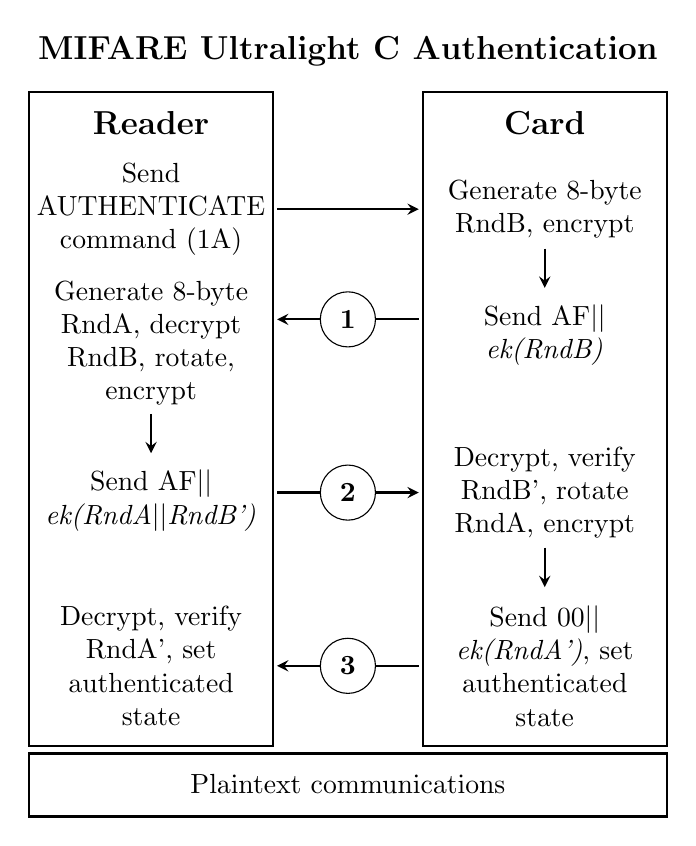
\begin{tikzpicture}[
    % Define styles
    box/.style={
        rectangle, 
        draw, 
        thick,
        minimum width=3.1cm, 
        minimum height=8.3cm,
        anchor=north
    },
    plaintext/.style={
        rectangle, 
        draw,
        thick,
        minimum width=8.1cm, 
        minimum height=0.8cm,
        anchor=north
    },
    arrow/.style={
        ->, 
        >=stealth,
        thick
    },
    numbered/.style={
        circle,
        draw,
        fill=white,
        minimum size=0.7cm,
        font=\bfseries
    }
]

% Set up the coordinate system
\def\yshift{0}

% Title
\node[font=\large\bfseries] at (-2.5,\yshift+4.0) {MIFARE Ultralight~C Authentication};
%\node[font=\large] at (-2.5,\yshift+4.0) {3-Pass Mutual Authentication};

% Draw reader box
\node[box, fill=none, anchor=north] (reader) at (-5,\yshift+3.5) {};
\node[font=\large\bfseries] at (-5,\yshift+3.1) {Reader};

% Draw card box
\node[box, fill=none, anchor=north] (card) at (0,\yshift+3.5) {};
\node[font=\large\bfseries] at (0,\yshift+3.1) {Card};

% Draw box for plaintext communication
\node[plaintext, fill=none, anchor=north] (card) at (-2.5,\yshift-4.9) {};

% Reader side texts
\node[align=center] at (-5,\yshift+2.0) {Send\\AUTHENTICATE\\command (1A)};
\node[align=center] at (-5,\yshift+0.3) {Generate 8-byte\\RndA, decrypt\\RndB, rotate,\\encrypt};
\node[align=center] at (-5,\yshift-1.7) {Send AF\textbar\textbar\\\textit{ek{(}RndA{\textbar}{\textbar}RndB'{)}}};
\node[align=center] at (-5,\yshift-3.8) {Decrypt, verify\\RndA', set\\authenticated\\state};

% Card side texts
\node[align=center] at (0,\yshift+2.0) {Generate 8-byte\\RndB, encrypt};
\node[align=center] at (0,\yshift+0.4) {Send AF\textbar\textbar\\\textit{ek{(}RndB{)}}};
\node[align=center] at (0,\yshift-1.6) {Decrypt, verify\\RndB', rotate\\RndA, encrypt};
\node[align=center] at (0,\yshift-3.8) {Send 00\textbar\textbar\\\textit{ek{(}RndA'{)}}, set\\authenticated\\state};

% Internal arrows in reader
\draw[arrow] (-5,\yshift-0.6) -- (-5,\yshift-1.1);
%\draw[arrow] (-4,\yshift-2) -- (-4,\yshift-3.8);

% Internal arrows in card
\draw[arrow] (0,\yshift+1.5) -- (0,\yshift+1.0);
\draw[arrow] (0,\yshift-2.3) -- (0,\yshift-2.8);

% Communication arrows between boxes
% Top arrow - Send Authenticate command
\draw[arrow] (-6+2.6,\yshift+2) -- (1-2.6,\yshift+2) node[midway, above, font=\small] {};
%\node[circle, draw, fill=white, minimum size=0.7cm, font=\bfseries] at (-2.5,\yshift+2) {1};

% First pass
\draw[arrow] (1-2.6,\yshift+0.6) -- (-6+2.6,\yshift+0.6) node[midway, below, font=\small] {};
\node[circle, draw, fill=white, minimum size=0.7cm, font=\bfseries] at (-2.5,\yshift+0.6) {1}; % 2

% Second pass
\draw[arrow] (-6+2.6,\yshift-1.6) -- (1-2.6,\yshift-1.6) node[midway, below, font=\small] {};
\node[circle, draw, fill=white, minimum size=0.7cm, font=\bfseries] at (-2.5,\yshift-1.6) {2}; % 3

% Third pass (top of the numbered ones)
\draw[arrow] (1-2.6,\yshift-3.8) -- (-6+2.6,\yshift-3.8) node[midway, below, font=\small] {};
\node[circle, draw, fill=white, minimum size=0.7cm, font=\bfseries] at (-2.5,\yshift-3.8) {3}; % 4

\node[align=center] at (-2.5,\yshift-5.3) {Plaintext communications};
\end{tikzpicture}

\captionsetup{hypcap=false}
\captionof{figure}{Three-pass mutual authentication process}
\label{fig:authprocess}
\vspace{3.0mm}
\setlength{\parindent}{15pt}

In real-world scenarios, many integrators assume that ephemeral operational constraints, such as timing restrictions, will prevent an adversary from relaying the tag's responses in time, which would allow message interception, modification, or injection without detection. As will be seen in the discussion of the relay attack, these assumptions do not hold up under careful examination with off-the-shelf security testing hardware. And since Ultralight~C lacks a CMAC messaging mechanism, there is no inherent method to ensure message integrity under relay attack.

\section{Relay Attack Against Ultralight~C}
\label{sec:relay}

Traditional relay attacks targeting RFID-based authentication systems typically face strict timing constraints imposed by the reader's communication protocols. These constraints require attackers to relay messages between the legitimate reader and a tag within precise timing windows to maintain synchronization and avoid authentication failures.

In contrast, the relay attack presented in this paper does not try to trick a reader into believing that, for example, a payment or an access control card is within close range. Instead, our goal is to unlock a tag by moving it to its \texttt{AUTHENTICATED} state.
Therefore, it capitalizes specifically on the authentication behavior of the tag itself, which notably lacks timeout constraints. Our work focuses explicitly on exploiting this characteristic by performing authentication solely with the tag, which waits indefinitely for responses from the reader.

We propose a practical relay attack implemented via two discrete relay devices: one positioned in proximity to a legitimate reader (Relay A) and the other placed near the MIFARE Ultralight~C tag (Relay B). Relay B initiates the authentication process by capturing the random challenge generated and encrypted by the tag (\texttt{RndB}), forwarding it through the relay channel to the legitimate reader. The reader subsequently responds with its encrypted challenge (consisting of \texttt{RndA} concatenated with a rotated \texttt{RndB'}), a message similarly relayed to the tag by Relay A. By forwarding these encrypted authentication messages, the attacker successfully induces the tag into an \texttt{AUTHENTICATED} state without physical proximity to the legitimate reader.

\vspace{5mm}
\hspace{-5mm}\resizebox{\columnwidth}{!}{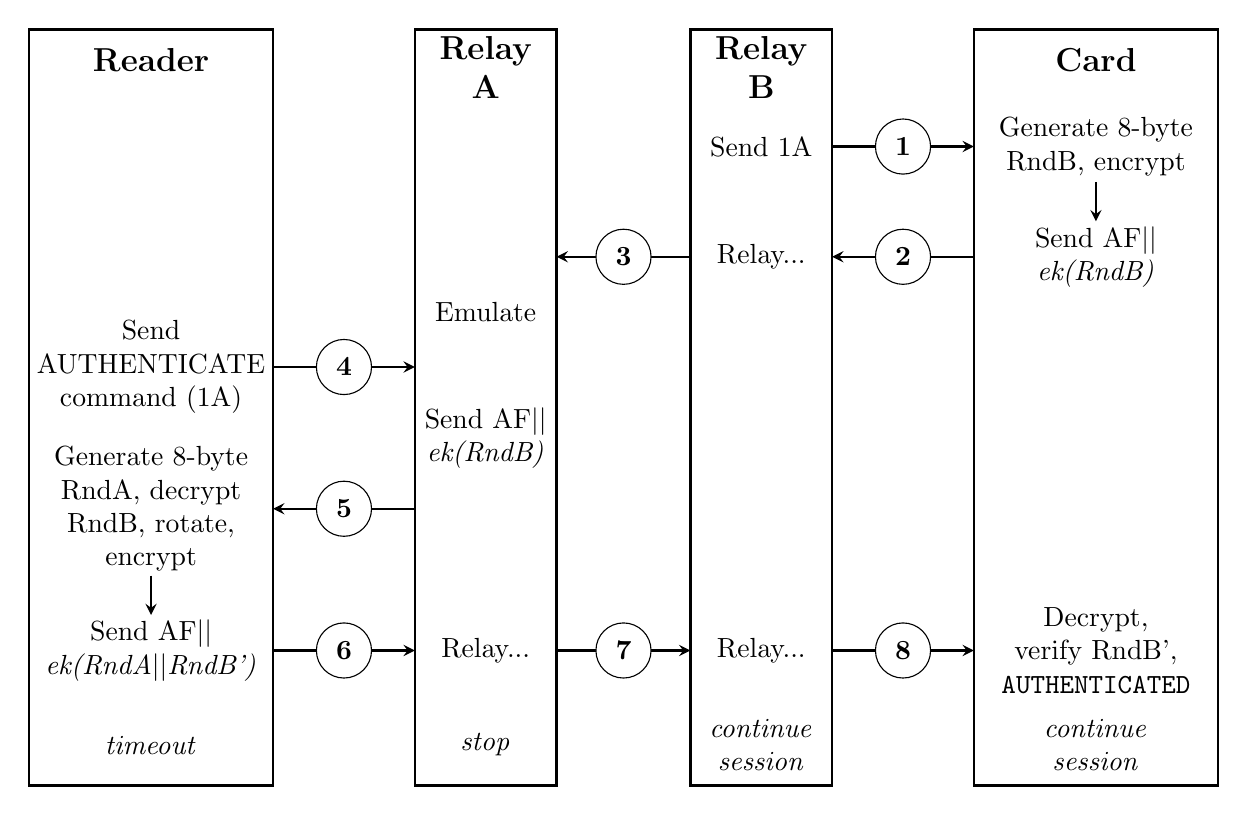
\begin{tikzpicture}[
    % Define styles
    box/.style={
        rectangle, 
        draw, 
        thick,
        minimum width=3.1cm, 
        minimum height=9.6cm,
        anchor=north
    },
    relaybox/.style={
        rectangle, 
        draw, 
        thick,
        minimum width=1.8cm, 
        minimum height=9.6cm,
        anchor=north
    },
    plaintext/.style={
        rectangle, 
        draw,
        thick,
        minimum width=8.1cm, 
        minimum height=0.8cm,
        anchor=north
    },
    arrow/.style={
        ->, 
        >=stealth,
        thick
    },
    numbered/.style={
        circle,
        draw,
        fill=white,
        minimum size=0.7cm,
        font=\bfseries
    }
]

% Set up the coordinate system
\def\yshift{0}
% Variables
\def\readerx{-6}
\def\boxwidth{3.1} % must match style
\def\relaywidth{1.8} % must match style
\def\relayAx{-1.75}
\def\relayBx{1.75}
\def\cardx{6}
\pgfmathsetmacro{\readerxE}{\readerx+\boxwidth/2}
\pgfmathsetmacro{\cardxW}{\cardx-\boxwidth/2}
\pgfmathsetmacro{\relayAxW}{\relayAx-\relaywidth/2}
\pgfmathsetmacro{\relayAxE}{\relayAx+\relaywidth/2}
\pgfmathsetmacro{\relayBxW}{\relayBx-\relaywidth/2}
\pgfmathsetmacro{\relayBxE}{\relayBx+\relaywidth/2}
\pgfmathsetmacro{\midBCx}{(\relayBxE+\cardxW)/2}
\pgfmathsetmacro{\midRAx}{(\relayAxW+\readerxE)/2}
\pgfmathsetmacro{\midABx}{0}
\def\steponey{\yshift+2}
\def\steptwoy{\yshift+0.6}
\def\stepfoury{\yshift-0.8}
\def\stepfivey{\yshift-2.6}
\def\stepsixy{\yshift-4.4}
\def\stepniney{\yshift-5.6}
\pgfmathsetmacro{\stepthreefoury}{(\steptwoy+\stepfoury)/2}
\pgfmathsetmacro{\stepfourfivey}{(\stepfoury+\stepfivey)/2}

% Title
% \node[font=\large\bfseries] at (0,\yshift+4.0) {Relaying MIFARE Ultralight~C Authentication};
%\node[font=\large] at (-2.5,\yshift+4.0) {3-Pass Mutual Authentication};

% Draw reader box
\node[box, fill=none, anchor=north] (reader) at (\readerx,\yshift+3.5) {};
\node[font=\large\bfseries] at (\readerx,\yshift+3.1) {Reader};

% Draw relay A
\node[relaybox, fill=none, anchor=north] (relaya) at (\relayAx,\yshift+3.5) {};
\node[align=center, font=\large\bfseries] at (\relayAx,\yshift+3) {Relay\\A};

% Draw relay B
\node[relaybox, fill=none, anchor=north] (relayb) at (\relayBx,\yshift+3.5) {};
\node[align=center, font=\large\bfseries] at (\relayBx,\yshift+3) {Relay\\B};

% Draw card box
\node[box, fill=none, anchor=north] (card) at (\cardx,\yshift+3.5) {};
\node[font=\large\bfseries] at (\cardx,\yshift+3.1) {Card};

\node[align=center] at (\relayBx,\steponey) {Send 1A};

\draw[arrow] (\relayBxE,\steponey) -- (\cardxW,\steponey) node[midway, above, font=\small] {};
\node[circle, draw, fill=white, minimum size=0.7cm, font=\bfseries] at (\midBCx,\steponey) {1};

\node[align=center] at (\cardx,\steponey) {Generate 8-byte\\RndB, encrypt};

\draw[arrow] (\cardx,\steponey - 0.45) -- (\cardx,\steptwoy + 0.45);

\node[align=center] at (\cardx,\steptwoy) {Send AF\textbar\textbar\\\textit{ek{(}RndB{)}}};

\draw[arrow] (\cardxW,\steptwoy) -- (\relayBxE,\steptwoy) node[midway, below, font=\small] {};
\node[circle, draw, fill=white, minimum size=0.7cm, font=\bfseries] at (\midBCx,\steptwoy) {2};

\node[align=center] at (\relayBx,\steptwoy) {Relay...};

\draw[arrow] (\relayBxW,\steptwoy) -- (\relayAxE,\steptwoy) node[midway, below, font=\small] {};
\node[circle, draw, fill=white, minimum size=0.7cm, font=\bfseries] at (\midABx,\steptwoy) {3};

\node[align=center] at (\relayAx,\stepthreefoury) {Emulate};

\node[align=center] at (\readerx,\stepfoury) {Send\\AUTHENTICATE\\command (1A)};

\draw[arrow] (\readerxE,\stepfoury) -- (\relayAxW,\stepfoury) node[midway, below, font=\small] {};
\node[circle, draw, fill=white, minimum size=0.7cm, font=\bfseries] at (\midRAx,\stepfoury) {4};

\node[align=center] at (\relayAx,\stepfourfivey) {Send AF\textbar\textbar\\\textit{ek{(}RndB{)}}};

\draw[arrow] (\relayAxW,\stepfivey) -- (\readerxE,\stepfivey) node[midway, below, font=\small] {};
\node[circle, draw, fill=white, minimum size=0.7cm, font=\bfseries] at (\midRAx,\stepfivey) {5};

\node[align=center] at (\readerx,\stepfivey) {Generate 8-byte\\RndA, decrypt\\RndB, rotate,\\encrypt};

\draw[arrow] (\readerx,\stepfivey - 0.85) -- (\readerx,\stepsixy + 0.45);

\node[align=center] at (\readerx,\stepsixy) {Send AF\textbar\textbar\\\textit{ek{(}RndA{\textbar}{\textbar}RndB'{)}}};

\draw[arrow] (\readerxE,\stepsixy) -- (\relayAxW,\stepsixy) node[midway, below, font=\small] {};
\node[circle, draw, fill=white, minimum size=0.7cm, font=\bfseries] at (\midRAx,\stepsixy) {6};

\draw[arrow] (\relayAxE,\stepsixy) -- (\relayBxW,\stepsixy) node[midway, below, font=\small] {};
\node[circle, draw, fill=white, minimum size=0.7cm, font=\bfseries] at (\midABx,\stepsixy) {7};

\draw[arrow] (\relayBxE,\stepsixy) -- (\cardxW,\stepsixy) node[midway, below, font=\small] {};
\node[circle, draw, fill=white, minimum size=0.7cm, font=\bfseries] at (\midBCx,\stepsixy) {8};

\node[align=center] at (\cardx,\stepsixy) {Decrypt,\\verify RndB',\\\texttt{AUTHENTICATED}};

\node[align=center] at (\relayAx,\stepsixy) {Relay...};

\node[align=center] at (\relayBx,\stepsixy) {Relay...};

\node[align=center] at (\readerx,\stepniney) {\emph{timeout}};

\node[align=center] at (\relayAx,\stepniney) {\emph{stop}};

\node[align=center] at (\relayBx,\stepniney) {\emph{continue}\\\emph{session}};

\node[align=center] at (\cardx,\stepniney) {\emph{continue}\\\emph{session}};

\end{tikzpicture}
}
\captionsetup{hypcap=false}
\captionof{figure}{Relayed authentication process}
\label{fig:authprocessrelay}
\vspace{3.0mm}
\setlength{\parindent}{15pt}

Each stage of the relay attack unfolds as follows:
\begin{enumerate}
    \item Relay B discovers the tag and its UID then sends the \texttt{AUTHENTICATE} (1A) command to the tag.
    \item The tag generates \texttt{RndB}, encrypts it (\textit{ek(RndB)}), and sends it back to Relay B.
    \item Relay B forwards the UID and \textit{ek(RndB)} to Relay A --- either asynchronously or synchronously --- using any suitable out-of-band communication channel, such as Wi-Fi, a sub-1 GHz RF transceiver, or end-to-end messaging apps.
    \item Relay A emulates the tag with the given UID and waits for the legitimate reader to initiate its own authentication by sending the \texttt{AUTHENTICATE} (1A) command.
    \item Relay A immediately responds to the reader with the captured \textit{ek(RndB)} received from Relay B.
    \item The reader decrypts \textit{ek(RndB)}, generates its own \texttt{RndA}, computes \texttt{RndB'}, and sends its response \textit{ek(RndA $||$ RndB')} back to Relay A.
    \item Relay A forwards \textit{ek(RndA $||$ RndB')} to Relay B.
    \item Relay B sends \textit{ek(RndA $||$ RndB')} to the tag.
    \item The tag decrypts \textit{ek(RndA $||$ RndB')}, verifies \texttt{RndB'}, and transitions to the \texttt{AUTHENTICATED} state.
\end{enumerate}
Crucially, the tag waits indefinitely after step 2 for the response from Relay B (sent by Relay A positioned at the reader). This eliminates the tight timing constraints typically associated with relaying reader-to-tag messages directly. The attacker successfully places the tag into an \texttt{AUTHENTICATED} state relative to the attacker's device (Relay B), without the need for direct interaction with the legitimate reader after step 6.
From the reader's perspective, the authentication process is aborted due to the lack of a response from the tag. This occurs when a tag is moved too quickly, and is therefore typically not regarded as a security incident.

Once the \texttt{AUTHENTICATED} state is established, the attacker effectively inherits the privileges of the legitimate reader until the field is removed or the tag performs a reset. This state serves as a foundational prerequisite for subsequent attacks, enabling the execution of arbitrary plaintext read and write commands against the tag.

Significantly, real-world deployments, such as those found in the hospitality and ticketing sectors, often leave memory lock bytes unset, inadvertently allowing attackers to overwrite pages. If the lock bytes permit overwriting the \texttt{AUTH0} page (42), writing the value \texttt{0x30} to the first byte fully unlocks the tag, enabling unrestricted reads and writes without authentication (except reading the key pages -- 44 to 47 -- which is always prevented). Consequently, attackers employing this relay attack technique can extract nearly the full memory contents of a tag and modify unlocked memory sections at will, enabling the partial key overwrite strategies and partial/full key recovery introduced in Section~\ref{sec:reduce}.

\section{Assessing Key Diversification in Deployed Systems}
\label{sec:kdf}

Many real-world systems rely on the uniqueness of the tag's 7-byte UID as input to a key derivation function (KDF), from which individual per-tag keys are derived. This practice prevents the compromise of one tag's key from affecting others, jeopardizing the security of the broader deployment. However, it is not always apparent to external observers whether a reader is applying key diversification.

We propose a practical process to test for UID-based key diversification using a relay comprising a tag emulator capable of changing its UID, such as a Proxmark3 or a Flipper Zero.
First, the original credential is presented directly to the reader to verify that its key is valid for the corresponding UID. Then, an emulator presents an arbitrary different UID value and attempts authentication again. If the system uses UID-based diversification, the authentication should fail with the modified UID, as the derived key will no longer match the reader's expectation. The detailed steps are described below.

\begin{enumerate}
    \item Present the original tag to the reader. Authentication should succeed.
    \item Perform the relay attack described in Section~\ref{sec:relay}, presenting a modified UID to the reader via an emulator while continuing to relay communication with the original tag in the background.
    \item Attempt to authenticate again.
    \begin{enumerate}
        \item If authentication with the tag \emph{fails}, it strongly indicates the system uses key diversification, as the key is tied to the UID. Do not relay the tag's negative response (NAK) to the reader.
        \item If authentication \emph{succeeds} even with the wrong UID, it strongly suggests the system uses a static key across all tags.
    \end{enumerate}
\end{enumerate}

This approach avoids the need to retrieve the actual key or compromise the tag itself; it simply checks if the system's authentication outcome changes when the UID is altered. It is important to note that performing such tests against live systems carries risks, as some readers may log or alarm on unexpected UIDs. However, if the attacker possesses multiple valid tag UIDs --- such as a second captured UID or is in possession of a second legitimate tag --- they can be used to bypass alarms or logging mechanisms that trigger on unknown UIDs while performing this technique.

\section{Identifying Site Key Diversification}
\label{sec:site_kdf}

While per-tag key diversification using the tag's UID is a common security measure, large-scale deployments across multiple physical locations or ``sites'' may introduce another layer of diversification: a unique site key. This practice ensures that a key recovered from a credential at one site cannot be used to compromise credentials at another, even if both sites use the same underlying system. Assessing whether a deployed system uses site-specific keys is crucial for understanding the broader impact of a key compromise and for identifying systems that may be viable targets for an attacker performing KDF reverse engineering.

The presence of site key diversification can be tested by attempting authentication at a secondary site known to use the same system, using a previously recovered credential. If the credential --- comprising the UID and its key --- is accepted, it demonstrates that both sites likely share a master key without site-specific diversification. Conversely, if authentication fails, it is an indication that the key derivation process incorporates a unique site key, rendering the recovered credential invalid outside of its original location.

An advantage of this method is that it does not require recovering a new key from the secondary site. Alternative approaches, such as relaying or sniffing a credential between sites, are often complex due to the geographic separation of distinct sites. The logistical challenge of accessing a live credential from another location exceeds that of recovering a single key using the methods described in this paper. Therefore, attempting authentication with a known UID and key pair is the most practical technique for identifying the extent of key diversification in widely deployed systems.

\section{Keyspace Reduction via 75\% Key Overwrite Relay}
\label{sec:reduce}

We introduce a relay-based partial key overwrite method that substantially reduces the effective keyspace for attacks against the two-key Triple Data Encryption Algorithm (2TDEA) implementation in MIFARE Ultralight~C. Although a complete brute-force search of the 112-bit 2TDEA keyspace is generally considered computationally infeasible, we identify and exploit a design oversight that significantly simplifies key recovery against deployments configured to use static keys. In Section~\ref{sec:kdf}, we demonstrated how it is possible to determine whether a system is using static or diversified keys prior to any key recovery attempt.

MIFARE Ultralight~C stores its 2TDEA key across four distinct memory pages (pages 44 through 47, or \texttt{0x2C} through \texttt{0x2F}). The key material consists of two independent 56-bit keys (Key1 and Key2), logically arranged such that pages 44-45 hold Key1 and pages 46-47 hold Key2. Critically, the tag's firmware does not enforce atomicity when writing to these key pages (via hardware or protocol); there is no mechanism requiring all four pages to be updated in a single, indivisible operation. Instead, each 4-byte page write is applied individually and immediately, allowing an attacker who has gained authenticated access via the previously described relay attack to strategically overwrite only selected portions of the key material.

This type of partial overwrite strategy against Ultralight~C was presciently explored by Ave and Socram in the RFID Love by Iceman Discord~\cite{discord} on October 10\textsuperscript{th}-12\textsuperscript{th}, 2020~\cite{discord_pko}. Although the discussion did not identify a full path to practical exploitability, the core idea -- partial key overwrite -- anticipated important elements of this attack and contributed to an early informal discussion of its feasibility. Partial key overwrite attacks that do not require invasive techniques, but instead exploit product design choices, have recently been extensively discussed in the context of microcontrollers~\cite{article3940}.

Exploiting this, we perform a ``75\% key overwrite'' through the previously described relay attack. Using the authenticated relay session, the attacker writes known values (e.g., all zeros) to three of the four key pages, leaving one 4-byte page (representing 25\% of the key material, or 28 effective bits) untouched. The key may be overwritten under the condition that the key blocks are still writable (bit 7 of lock byte 3 is zero). The attacker is then able to carry out an online brute-force attack against the remaining $2^{28}$ possibilities to recover a quarter of the 2TDEA key (an estimated time frame for this attack is provided in Section~\ref{sec:estimate}). By combining four recovered key fragments -- each corresponding to a different quarter of a known static key (established in Section~\ref{sec:kdf}) -- the entire 112-bit effective 2TDEA key can be reconstructed from a minimum of four tags.

\vspace{2mm}
The partial overwrite procedure, targeting a different key page on each tag, is as follows:
\begin{itemize}
    \item Tag 1: Overwrite pages 45, 46, 47. Brute-force page 44 ($2^{28}$ attempts).
    \item Tag 2: Overwrite pages 44, 46, 47. Brute-force page 45 ($2^{28}$ attempts).
    \item Tag 3: Overwrite pages 44, 45, 47. Brute-force page 46 ($2^{28}$ attempts).
    \item Tag 4: Overwrite pages 44, 45, 46. Brute-force page 47 ($2^{28}$ attempts).
\end{itemize}
\vspace{2mm}

Even in configurations employing key diversification through KDFs, this technique remains valuable. Partial recovery can reveal whether portions of the derived keys remain static or show consistent changes across multiple tags, indicating the complexity or simplicity of the underlying derivation scheme. Such observations can inform attackers about whether the integrator has used a sophisticated cryptographic derivation function such as the ones recommended in AN10922~\cite{nxp_an10922} or a simpler, potentially insecure method, thereby aiding subsequent cryptanalysis.

Notably, Ultralight~C lacks an authentication failure counter that could limit the effectiveness of brute-force attacks, for example, by locking out the tag when it meets a threshold, or exponentially increasing tag response times. This omission in Ultralight~C allows attackers unlimited online authentication attempts, undermining the remaining security offered by the reduced 28-bit keyspace. An optional authentication failure counter feature was introduced in the subsequent MIFARE Ultralight~EV1 and Ultralight~AES (MF0ICU2 successor) ICs, recognizing the value of limiting brute-force attempts. Interestingly, an authentication failure counter is also absent in the MIFARE Plus product line (which is not in the scope of this article).

\section{Further Keyspace Reduction via Tearing}
\label{sec:tear}

MIFARE Ultralight~C tags implement anti-tearing mechanisms to protect memory areas such as the 16-bit counter, OTP and lock bit pages~\cite{nxp_an12265}. However, the key pages do not benefit from the same level of protection, making them vulnerable to tearing attacks.

Prior reduction of the keyspace to $2^{28}$ bits -- achieved through the 75\% key overwrite technique -- can be further reduced by leveraging EEPROM tearing attacks~\cite{teuwen2021eeprom}. These methods exploit the physical characteristics of EEPROM write operations, specifically targeting the initial erase phase inherent in MIFARE Ultralight~C's write process, where a page is first zeroed before new data is written.

\subsection{Tearing Attack Principles}

EEPROM tearing attacks exploit the non-atomic nature of memory write operations. When an EEPROM write or erase operation is interrupted, it affects the number of trapped electrons in the floating gates of transistors, which in turn affects the logical value when read back. 

By precisely timing the interruption of the erase phase -- a technique known as tearing -- an attacker can induce a partial zeroing of the target key page. Consequently, only the bits that remain non-zero need to be recovered, further reducing the effective keyspace below the already constrained $2^{28}$ bits and accelerating online brute-force attacks, particularly when multiple tags share a static key.

This strategy requires many authentications to overwrite key pages, unless \texttt{AUTH0} is configured to allow unauthenticated writes. Therefore, it is strongly recommended to use the \texttt{AUTHENTICATED} relay state to modify the \texttt{AUTH0} value to at least 48 (\texttt{0x30}) if not already set. This requires \texttt{AUTH0} to be writable (bit 5 of lock byte 3 is zero).

\subsection{Environmental Manipulation of Weak Bits}
\label{sec:envweak}
A gate loaded with a number of electrons leading to a threshold voltage very close to the reference threshold voltage can be read as a 1 or a 0 across several reads, with some probability gradient related to the actual amount of charge. These partially erased bits, often referred to as ``weak bits,'' provide additional avenues for exploitation.

The probability to read a weak bit as a 0 or a 1 can be influenced by the distance to the reader and the temperature. An attacker might manipulate these conditions to influence the read outcome. For example, by positioning the tag to maximize the number of bits read as '0' (potentially at a greater distance), the attacker can perform an initial brute-force prioritizing low Hamming weight keys. Subsequently, altering the conditions (e.g., moving closer to the reader or heating the tag) might cause some weak bits to be seen again as '1'. New brute-force attempts at several environmental conditions can then focus specifically on identifying the bits that reverted, effectively providing multiple opportunities to recover the key material from a single torn state.

Temperature also affects EEPROM erase and write operation speeds. Our experiments showed that heat resulted in more frequent bitflips during tearing operations on both NXP Ultralight~C and Ultralight~AES tags. This temperature dependency can be exploited to fine-tune the tearing process for optimal results.

\subsection{Characterizing Late-erasing Bits}
\label{sec:lateerase}
Additional key bits can be inferred by characterizing late-erasing bits. Once a segment has been partially exploited to reveal some key bits, writing the value \texttt{0xFFFFFFFF} to the page and performing progressive tearing allows identification of which bits erase later. If a bit erases later than the already-recovered bits, it likely represents a '0' in the original key; otherwise, we assume it would have been recovered in earlier attempts. This information further constrains the brute-force search space.
Unlike the recovered '1' bits, the '0' bits inferred by this method are not guaranteed to be correct. Therefore, these inferred '0' bits must be treated with caution, particularly when timing differences are small, and this uncertainty must be accounted for in subsequent brute-force attempts.

\subsection{Calibration and Implementation}
\label{sec:tearing_calibration}
To refine the tearing process, calibration can be performed on other writable pages.
By testing tearing on other unlocked memory pages (non-key pages), an attacker can approximate the necessary timing offsets and predict the likely number of bits affected during a tear on the actual key material. This calibration leverages the principle that EEPROM erase/write characteristics, while having some variability, exhibit reproducible tendencies related to timing and physical factors.

Knowing that there are only 3683 28-bit key candidates with a Hamming weight $HW\leq 3$ (407 if limited to $HW\leq 2$), which takes a few seconds to process, the attack can proceed as follows.

\begin{enumerate}
    \item After zeroing non-targeted segments, initiate a write command to the final key quarter page (the specific data value is irrelevant)~;
    \item Interrupt the operation during the erase phase, aiming to partially clear some of the existing key bits~;
    \item Perform a quick online brute-force attack with key candidates\footnote{In practice, the key value is not strictly stable and monotonic bitwise across tearing operations. It is better to test several times the most probable candidates and to test candidates with a Hamming distance close to the previous valid key value, with bitflips in both directions.} of $HW\leq 2$ or 3~;
    \item If it fails, tear again to reduce the segment further~;
    \item If the key becomes zero, it is likely that the segment was torn excessively and we can try to revive a few bits of that tag with the environment manipulations~;
    \item If it succeeds, try to revive a few bits and to brute-force the new key, based on the previously found key but with a slightly higher HW, to reveal more bits.
\end{enumerate}

The process is then repeated on a few tags, each one revealing a few '1' bits of the key as each tag EEPROM has its own behavior.
After processing these few tags, a bitmask is constructed by combining the partially erased keys revealed by each tag with a bitwise OR operation, as bits previously identified as '1' can be assumed correct.
Then, the attack focuses only on recovering the bits that were initially '0' or were flipped to '0' during the tearing event. An efficient implementation for enumerating supersets of the known bitmask is presented below.

\begin{lstlisting}[style=customc]
// Base mask before tearing is 0x01010101 in hex 
// (LSB of each byte is ignored - 3DES parity bits)
void iterate_supersets(uint32_t base_mask) {
    uint32_t zero_positions = ~base_mask;
    uint32_t subset = 0;
    while (1) {
        print_binary(base_mask | subset);
        if (subset == zero_positions)
            break;
        subset = (subset - zero_positions) & zero_positions;
    }
}
\end{lstlisting}
Some trade-offs need to be made when choosing the timing offsets: if many tags are available, we can use aggressive timings to get faster results, but at the cost of fewer recovered bits on average. Thus, we managed to recover an average of 1.5 bits in 10 seconds per tag.
Alternatively, one may consider slowly tearing the four segments in each step until a total $HW\leq 2$ or 3, then trying to revive some bits anywhere in the four segments. But the number of 112-bit key candidates with Hamming weight $HW\leq 3$ is much larger than for a single segment: 234249 (6329 if limited to $HW\leq 2$).
Moreover, experiments indicate that comparatively few bits can be revived across four segments versus tearing and reviving a single segment.

\subsection{Practical Implementation on Resource-Constrained Devices}

Tearing attacks can be implemented even on less precise, low-compute hardware such as the Flipper Zero. By implementing a critical section with a busy loop for timing control, tearing an EEPROM erase operation at multiple states can be achieved. The search space reduction from $2^{28}$ depends on the precision of the hardware in an attempt to leave only a reduced number of bits set to '1'. While the Flipper Zero might achieve a sufficiently low number of '1's to be quickly exploited in an online brute-force, more precise equipment like the Proxmark3 can achieve more reliable outcomes, though the computational resources of the connected host typically make such optimizations unnecessary for some of the (later) discussed attacks.

\subsection{Impact on Attack Complexity}

The combination of the 75\% key overwrite technique with tearing attacks dramatically reduces the computational requirements for key recovery. With sufficient source tags and proper calibration of the tearing process, the online brute-force time can be reduced from days to minutes (as discussed later in Section~\ref{sec:estimate}), making the attack practical even with limited computational resources. This technique is applicable to both Ultralight~C and Ultralight~AES, though the specific timing parameters and success rates may vary between implementations.

\section{Improved Attack by Collecting a Reader Nonce}
\label{sec:readernonces}
The 75\% key–overwrite relay attack method still demands an online search of $2^{28}$ candidates against four physical tags. By collecting the reader's contribution to a single authentication challenge (forming a nonce pair) we can reduce the number of source tags required to expose a static deployment key to three or two tags, by respectively migrating 25\% or 50\% of the search entirely offline.

During mutual authentication, the tag first returns $c_{1}=E_{K}(\mathtt{RndB})$. The reader then sends $c_{2}=E_{K}(\mathtt{RndA}\Vert\mathtt{RndB}')$, where $\mathtt{RndB}'$ is a one-byte left rotation of the decrypted $\mathtt{RndB}$. Finally, if the tag can validate the reader response, it returns  $c_{3}=E_{K}(\mathtt{RndA}')$, similarly having applied a one-byte left rotation on $\mathtt{RndA}$. Once respectively three or two key pages have been discovered via an online attack, the remaining $2^{28}$ or $2^{56}$ candidates for the final page(s) can be tested offline: decrypt $c_{1}$ and $c_{2}$ with a candidate key $K'$, verify that the rotation relation holds, and accept on a match.

Collecting $(c_{1},c_{2})$ is straightforward. An emulator chooses an arbitrary $c_{1}$ to reply to the reader \texttt{AUTHENTICATE} command, then captures $c_{2}$ from the reader. Then the attacker simply terminates the exchange --- most commercial readers ignore or silently log an incomplete third pass, leaving no operational trace.

Similarly, one can collect $c_2$ and $c_3$ to mount an offline search for a matching $\mathtt{RndA}$, however, this requires an adversary to sniff the reader authentication exchange with a valid tag configured with the target key.

The offline search of one segment is implemented in the \texttt{mfulc\_des\_brute} utility accompanying this paper (see Appendix~\ref{app:tools}), which accepts an arbitrary $(c_{1},c_{2})$ pair and checks the rotation predicate described above. Because all work is offline, the search scales linearly with available CPU or GPU resources and completes in practical time on commodity hardware.

An attacker can therefore perform a hybrid online and offline attack to assemble the full 112-bit key, instead of an exhaustive online attack against all four quarters of the key. Offloading the computation using this strategy reduces the attack window from hours or days of interrogating the final segment(s) from the tag to a time frame which fits comfortably within the capabilities of an ordinary desktop computer. When combined with tearing techniques that further reduce the offline search space, the two-tag variant remains well within the same practical resource and time constraints.

\section{Optimizing Brute-Force Attacks}
\label{sec:optimize}
The preceding sections establish that partial key overwrites can reduce the brute-force search space to a manageable size. However, the practical feasibility of the attack depends on the speed at which key candidates can be tested. This section details several optimizations that accelerate both the online and offline phases of the brute-force attack. By exploiting protocol-level shortcuts and the cryptographic structure of 2TDEA, we demonstrate how to minimize latency during online interactions with the tag and reduce the computational workload for offline key searching, further lowering the barrier for a successful attack.

\subsection{Online Enhancements}
\label{sec:onlineoptimize}
After three of the four key pages have been overwritten, recovering the remaining \(2^{28}\) candidates for the last quarter of the 2TDEA key is an online exercise in repeatedly forcing the tag back into the \texttt{ACTIVE} state and observing whether the final pass of the three-way handshake is returned by the tag. Three protocol observations reduce the per-trial latency. First, when an authentication attempt fails the tag answers with a NAK but remains powered in the \texttt{HALT} state; a single \texttt{WUPA} command re-primes the tag and places it in the \texttt{READY} state --- there is no need to cycle the RF field.  Second, issuing a direct \texttt{READ~0x00} immediately after \texttt{WUPA} performs the cascade-level selection implicitly and leaves the tag in the \texttt{ACTIVE} state, eliminating the ordinary anticollision sequence. From this point the \texttt{AUTHENTICATE} command tests the next key candidate; success returns the encrypted \(\texttt{RndA}'\) and the tag is in the desired \texttt{AUTHENTICATED} state, while failure yields a NAK and the loop repeats.
Third, to minimize the computational latency of the reader performing the online brute-force attack, all cryptographic operations over \texttt{RndA} can be skipped. It is not necessary to decrypt the final tag response (\textit{ek(RndA')}) --- a successful authentication can be inferred by checking the length of the returned data --- nor is it required to even encrypt \texttt{RndA} in the initial reader response, as the properties of CBC mode allow us to encrypt the second block directly without encrypting the first block.
This approach reduces the total number of 3DES block operations per key candidate from four to two.

\begin{center}
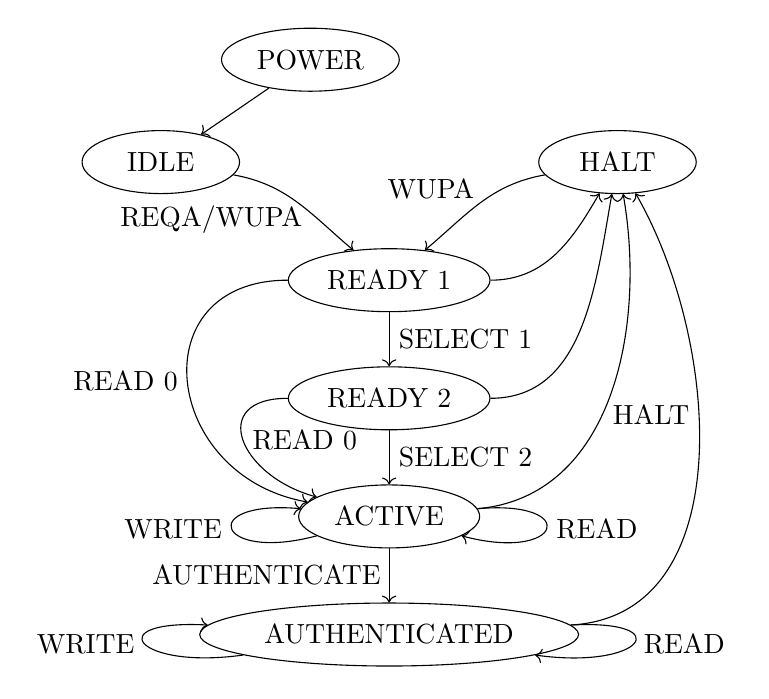
\begin{tikzpicture}[
    node distance=1.5cm,
    state/.style={ellipse, draw, minimum width=2cm, minimum height=0.8cm},
    every edge/.style={draw, ->, >=stealth}
]

% States
\node[state] (por) at (-3,5.8) {POWER};
\node[state] (idle) at (-4.9,4.5) {IDLE};
\node[state] (halt) at (0.9,4.5) {HALT};
\node[state] (ready1) at (-2,3) {READY 1};
\node[state] (ready2) at (-2,1.5) {READY 2};
\node[state] (active) at (-2,0) {ACTIVE};
\node[state] (authenticated) at (-2,-1.5) {AUTHENTICATED};

% Transitions
\draw[->] (por) -- (idle);
\draw[->] (idle) to[out=-10, in=140, looseness=1] node[pos=0.7] {\hspace{-7.8em}REQA/WUPA} (ready1);
\draw[->] (halt) to[out=190, in=40, looseness=1] node[pos=0.3] {\hspace{-5.2em}WUPA} (ready1);

% SELECT transitions
\draw[->] (ready1) -- node[right, align=left] {SELECT 1} (ready2);
\draw[->] (ready2) -- node[right, align=left] {SELECT 2} (active);

% Left curved transitions
\draw[->] (ready1) to[out=180, in=170, looseness=1.7] node[left, align=right] {READ 0} (active);
\draw[->] (ready2) to[out=180, in=165, looseness=2] node[right, align=left] {READ 0} (active);

\draw[->] (active) to[out=195, in=175, looseness=8.5] node[left, align=right] {WRITE} (active);
\draw[<-] (active) to[out=-15, in=5, looseness=8.5] node[right, align=left] {READ} (active);

% AUTHENTICATE transition
\draw[->] (active) -- node[right, align=left] {\hspace{-9.0em}AUTHENTICATE} (authenticated);

% HALT transitions
\draw[->] (ready1) to[out=0, in=240, looseness=1] node[right, pos=0.6] {} (halt);
\draw[->] (ready2) to[out=0, in=260, looseness=1] node[right, pos=0.6] {} (halt);
\draw[->] (active) to[out=5, in=280, looseness=1] node[above, pos=0.7] {} (halt);
\draw[->] (authenticated) to[out=3, in=300, looseness=1] node[above, pos=0.55] {\hspace{-3.5em}HALT} (halt);

% Self-loop for AUTHENTICATED
\draw[<-] (authenticated) to[out=-8, in=3, looseness=6.0] node[right, align=left] {READ} (authenticated);
\draw[->] (authenticated) to[out=188, in=177, looseness=6.0] node[left, align=right] {WRITE} (authenticated);

% Right side vertical line and labels
%\draw[->] (3.5,6.5) -- (3.5,0.5);
%\node[align=left] at (2.5,3.5) {selection\\procedure};
%\node[align=left] at (2.5,0) {memory\\operations};
%\draw[->] (3.5,0.4) -- (3.5,-2.0);

\end{tikzpicture}

\vspace{1mm}\newline
\captionsetup{hypcap=false}
\captionof{figure}{Reference state diagram for MIFARE Ultralight~C operation}
\end{center}

Key candidates are optimally iterated using the \texttt{iterate\_supersets} function introduced in Section~\ref{sec:tear}. Together with the protocol shortcuts outlined above, this strategy sustains a throughput of at least 100 authentication attempts per second even on resource-constrained hardware such as the Flipper Zero. This yields a speedup of approximately 12.5$\times$ relative to the unoptimized baseline implementation on the Flipper Zero, which processed only 8 authentication attempts per second.

Ultralight~C provides no authentication-failure counter (discussed in Section~\ref{sec:reduce}, so an attacker may perform an unlimited sequence of trials. Each attempt interacts with the non-volatile memory only through \textit{read} operations; the EEPROM's write endurance therefore remains untouched. Empirical testing further confirms that millions of consecutive \texttt{READ~0x00} operations cause no measurable degradation, so an online brute-force attack inflicts virtually no physical wear on the IC. When these properties are coupled with the reduced search spaces obtained via partial key overwrite or tearing techniques, an online brute-force attack becomes tractable on modest hardware. Total estimated time of a key recovery is discussed in Section~\ref{sec:estimate}.

\subsection{Offline Enhancements}
\label{sec:offlinetdes}
The computational cost of the offline brute-force attack in Section~\ref{sec:readernonces} can be reduced by optimizing key recovery. The two-tag variant, which recovers the final 56 bits offline, is especially suited to this. By choosing which half of the 2TDEA key to recover online --- specifically targeting Key1 (pages 44–45) --- the offline search for Key2 (pages 46–47) becomes appreciably more efficient.

This optimization arises from the structure of 2TDEA decryption, which follows a Decrypt-Encrypt-Decrypt (D-E-D) sequence using the keys (Key1, Key2, Key1), as illustrated in Figure~\ref{fig:desede}. With Key1 known from the online phase, the initial decryption step, $D_{\mathrm{Key1}}(C)$, can be performed once as a pre-computation on the captured nonce-pair ciphertexts ($c_1$ and $c_2$). The main brute-force loop, which iterates through all $2^{56}$ candidates for Key2, is thus simplified. For each guess of Key2, only the remaining two operations --- $E_{\mathrm{Key2}}$ on the pre-computed intermediate value, followed by the final $D_{\mathrm{Key1}}$ --- are required to produce a plaintext candidate for validation.

\begin{center}
\hspace{4mm}
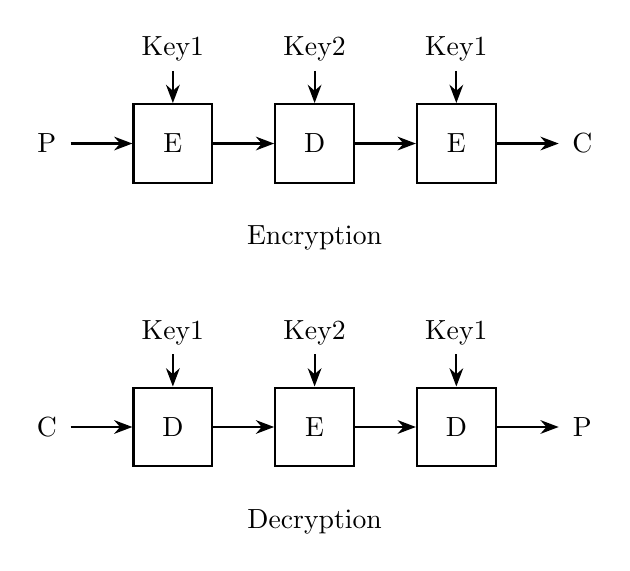
\begin{tikzpicture}[
    box/.style={draw, rectangle, minimum width=1cm, minimum height=1cm, thick},
    arrow/.style={->, >=Stealth, thick},
    label/.style={font=\normalsize}
]

% Encryption section
\node[label] at (-0.8, 1.8) {P};
\node[box] (E1) at (0.8, 1.8) {E};
\node[box] (D) at (2.6, 1.8) {D};
\node[box] (E2) at (4.4, 1.8) {E};
\node[label] at (6, 1.8) {C};

% Keys for encryption
\node[label] (K1a) at (0.8, 3) {$\mathrm{Key1}$};
\node[label] (K2a) at (2.6, 3) {$\mathrm{Key2}$};
\node[label] (K1b) at (4.4, 3) {$\mathrm{Key1}$};

% Arrows for encryption
\draw[arrow] (-0.5, 1.8) -- (E1);
\draw[arrow] (E1) -- (D);
\draw[arrow] (D) -- (E2);
\draw[arrow] (E2) -- (5.7, 1.8);
\draw[arrow] (K1a) -- (E1);
\draw[arrow] (K2a) -- (D);
\draw[arrow] (K1b) -- (E2);

% Encryption label
\node[label] at (2.6, 0.6) {Encryption};

% Decryption section
\node[label] at (-0.8, -1.8) {C};
\node[box] (D1) at (0.8, -1.8) {D};
\node[box] (E3) at (2.6, -1.8) {E};
\node[box] (D2) at (4.4, -1.8) {D};
\node[label] at (6, -1.8) {P};

% Keys for decryption
\node[label] (K1c) at (0.8, -0.6) {$\mathrm{Key1}$};
\node[label] (K2b) at (2.6, -0.6) {$\mathrm{Key2}$};
\node[label] (K1d) at (4.4, -0.6) {$\mathrm{Key1}$};

% Arrows for decryption
\draw[arrow] (-0.5, -1.8) -- (D1);
\draw[arrow] (D1) -- (E3);
\draw[arrow] (E3) -- (D2);
\draw[arrow] (D2) -- (5.7, -1.8);
\draw[arrow] (K1c) -- (D1);
\draw[arrow] (K2b) -- (E3);
\draw[arrow] (K1d) -- (D2);

% Decryption label
\node[label] at (2.6, -3) {Decryption};

\end{tikzpicture}

\vspace{1mm}\newline
\captionsetup{hypcap=false}
\captionof{figure}{Two-key Triple DES (2TDEA) structure}
\label{fig:desede}
\end{center}

Moreover, out of the two blocks of $c_2$, only the second is useful for the attack, and CBC mode decryption allows us to decrypt the second block directly. Under CBC mode, decryption of block \(i\) is given by
\[
P_i = D_K(C_i) \oplus C_{i-1},
\]
where \(D_K(\cdot)\) denotes the block-cipher decryption under key \(K\). Hence, computing the block-cipher decryption of the second ciphertext block and XORing that intermediate value with the first ciphertext block directly produces the second plaintext block, eliminating any dependence on decrypting the preceding block.

These methods reduce the total number of single DES operations per key candidate from nine to four. Consequently, the total computational cost for the offline search is reduced by approximately 55\%. This optimization materially lowers the time and cost required for the offline attack, as reflected in the practical estimates presented in Section~\ref{sec:estimate}, and makes the two-tag full key recovery method more practical in realistic scenarios targeting systems with static keys.

\section{Counterfeit Ultralight~C Cards}
\label{sec:counterfeit}
The widespread adoption of the MIFARE portfolio has led to the emergence of a market for counterfeit cards that embed compatible integrated circuits. These products often mimic the form factor and command structure of genuine NXP products, yet they include implementation flaws which render them significantly more vulnerable to attack. Our investigation has confirmed that these counterfeit products have successfully penetrated legitimate supply chains, including within the hospitality sector. In addition, we identified certain sellers advertising counterfeit products as genuine NXP cards, displaying the NXP logo. The proliferation of such cards, infringing trademarks or maintaining a certain ambiguity on their true nature, poses a substantial, often unrecognized, risk to the security of deployed systems. NXP has publicly acknowledged this threat and has engaged in ongoing legal actions to protect its intellectual property against infringing manufacturers and distributors, such as Global Card Systems~\cite{nxp_mifare_anticounterfeit}. Our analysis focused on several widely circulated counterfeit cards, primarily those featuring Giantec GT23SC4489~\cite{ulcg_datasheet}, Feiju FJ8010~\cite{fj8010}, and USCUID-UL ICs. Although Mikron MIK1K5PTAC~\cite{mik1k5ptac} and Feiju F8213C/F8216C~\cite{f8216c} with their variants have been reported, we could not include them in our evaluation because we were unable to source samples.

\subsection{Giantec GT23SC4489 aka ULCG}
\label{sec:giantec}
The Giantec GT23SC4489 is a product that is particularly noteworthy due to its frequent occurrence in real-world deployments, especially within the hospitality industry ($\approx$ 29\% of observed cards, $n=73$). In circulation as early as 2014~\cite{ulcg_datasheet}, and discovered in 2018~\cite{ulcg_gh_issue}, it is easily identifiable by its UID suffix (ending in \texttt{1589}). Some major hotel chains explicitly label these cards as ``ULCG'' cards. We will use the terms GT23SC4489 and ULCG interchangeably from now on.

Our analysis identified its hardware origins through decapping and analysis of the IC markings.

\vspace{0.5em}
\noindent
\begin{minipage}{\linewidth}
    \centering
    \includegraphics[width=\linewidth]{overview_gt5620am1c}
    \captionsetup{hypcap=false}
    \captionof{figure}{Overview of GT23SC4489 IC}
\end{minipage}

\vspace{0.5em}
\noindent
\begin{minipage}{\linewidth}
    \centering
    \includegraphics[width=\linewidth]{gt5620am1c_closeup}
    \captionsetup{hypcap=false}
    \captionof{figure}{Close-up of GT23SC4489 IC including manufacturer logo and part number (GT5620AM1C)}
\end{minipage}
\vspace{0.5em}

The primary vulnerability of the GT23SC4489 is its weak pseudo-random number generator. Instead of the secure true random number generator (TRNG) found in genuine NXP ICs~\cite{Merhi2011}, ULCG employs a simple and predictable linear-feedback shift register (LFSR). Its deterministic output enables attacks that exploit the card's predictable challenge (\texttt{RndB}) during authentication. We reverse-engineered the LFSR responsible for generating \texttt{RndB} and identified it as a 16-bit linear-feedback shift register, described by the following equation.

\begin{equation}
\begin{array}{l}
x = \bigl(x \ll 15\bigr) \;\big\vert\; \\ \Bigl(\bigl(x \gg 1\bigr) \oplus
\quad \bigl(\bigl((x \gg 3) \oplus (x \gg 4) \oplus (x \gg 6)\bigr) \;\&\; 1\bigr)\Bigr)
\end{array}
\end{equation}

Here, $x$ is a 16-bit register, and each new challenge 16-bit word is derived by iterating this transformation. One would expect that the transformation is iterated 16 times to entirely renew the state for each new word, but this is not the case, and most of the state content is repeating in successive words. For example, when writing down the bits of the nonce \texttt{0xCC0C6607B303D981}, we clearly see the repetitions.
\begin{center}
\begin{tabular}{l}
\texttt{~~~11001100000011~0~\textbf{0}}\\
\texttt{~~\textbf{0}1100110000001~1~\textbf{1}~}\\
\texttt{~\textbf{1}0110011000000~1~\textbf{1}~~}\\
\texttt{\textbf{1}1011001100000~0~1~~~}\\
\end{tabular}
\end{center}

The LFSR resembles the MIFARE Classic 16-bit LFSR with one small difference: it is as if its state was stored rotated one bit to the left.
Not only does the number of possible nonce values drop from $2^{64}$ to $2^{16}-1$, but the situation is compounded by the absence of a truly random seed. Indeed, the actual nonce value appears to depend primarily on the time spent between sending the wake-up command (\texttt{REQA} or \texttt{WUPA}) and querying it for its nonce.

\begin{center}
    \resizebox{1.0\linewidth}{!}{version https://git-lfs.github.com/spec/v1
oid sha256:23b9c2e0e00cea8b2b02afc7fb29f16d919643377645eeea9714422387087160
size 507907
}
    \captionsetup{hypcap=false}
    \captionof{figure}{Initial \texttt{RndB} observed across 10\,000 authentication attempts on a GT23SC4489.}
    \label{fig:freq_distrib_ulcg}
\end{center}

Figure~\ref{fig:freq_distrib_ulcg} illustrates this issue: in 10\,000 requests, all LFSR indexes of the observed nonce values fell in the gray zone of the graph and most of them highly concentrated in an even smaller portion of about $2^{7}$ values.
In practice, many \texttt{RndB} values will recur within a small number of transactions. Given the observed bias, there is a greater than 50\% chance of finding a duplicate among 12 nonces, and the probability reaches 99.99\%  with only 39 nonces. This repetition drastically eases offline analysis, since an attacker can gather multiple repeated \texttt{RndB} values and match them with partial key guesses offline. While the official NXP TagInfo application warns users about some of the non-genuine cards\footnote{Note that the TagInfo detection is quite unreliable on Ultralight~C cards and will, for example, detect old genuine NXP cards as \emph{``Non-genuine, most probably counterfeit product''}, solely based on their old ``site'' reference in the UID (tested on NXP TagInfo v6.1.0).}
, many systems neither check nor block usage of non-genuine cards.

This weakness is compounded by the card's lack of effective anti-tearing mechanisms for its memory. Unlike genuine NXP cards that protect critical pages like the lock bytes from interrupted write commands, the GT23SC4489 is vulnerable to tearing attacks that can disable these security configurations. An attacker can exploit this to unlock the card and modify its memory contents at will after gaining authenticated access via a relay attack, even where the memory lock bytes were properly configured.

The combination of a predictable PRNG and insecure memory protection enables a complete key recovery from a single ULCG card. By obtaining a single valid response from a legitimate reader (either with a replay of a frequent card nonce, or sniffing an authentication exchange) and collecting a series of challenges, an attacker can perform a rapid offline brute-force search --- as detailed later in Section~\ref{sec:counterfeit_recovery}. Our practical tests demonstrated that a full key can be recovered in under one minute on a standard laptop, and in as little as fifteen seconds on a modern desktop computer. Additional benchmarks are provided in Section~\ref{sec:estimate}. This rapid compromise underscores the significant risk posed by the deployment of these compatible ICs.

\subsection{USCUID-UL}
\label{sec:uscuidul}
Another counterfeit product identified during our investigation is based on an unknown IC and found in hospitality deployments ($\approx$ 5\% of observed cards, $n=73$). Our analysis began with two unmarked ICs (cf Figures~\ref{fig:uscuidulv1ic} and~\ref{fig:uscuidulv2ic}) that functioned similarly to a standard MIFARE Ultralight~C but exhibited unique command responses and processing times that distinguish them from genuine NXP ICs. These specific anomalies precisely matched the behavior of a known USCUID-UL card when configured to emulate a standard Ultralight~C.

USCUID-UL cards are configurable `magic' cards, which allows their UID and other parameters to be altered. This led to our hypothesis that the initial unmarked ICs are USCUID-UL cards that have been 'locked down' into a non-configurable state. Subsequent decappings of known USCUID-UL cards acquired from various sources revealed three IC layouts: two corresponding to Figures~\ref{fig:uscuidulv1ic} and~\ref{fig:uscuidulv2ic}, and a third one (cf Figure~\ref{fig:unlockedic}) featuring a few die markings. Although the specific manufacturer remains unidentified, the profound architectural similarities at the silicon level between the marked and unmarked ICs --- as well as an intersecting fingerprint --- allow us to establish a definitive link.

Public shipping records of hospitality deployments suggest that their supply chain may involve manufacturers such as Chengdu Mind or Global Card Systems. Microscopic analysis of the third USCUID-UL IC reveals various markings, including ``HNU,'' ``X\&H,'' and ``ZSMicro,'' as shown in Figures \ref{fig:unlockedic}, \ref{fig:unlockedicmarkings}, and \ref{fig:unlockediczsmicro}.

Similar to the Giantec GT23SC4489, it employs a predictable 16-bit linear-feedback shift register instead of a secure TRNG.

\pagebreak

We reverse-engineered this LFSR using the Berlekamp–Massey algorithm and found it to be identical to the one used in the MIFARE Classic. Its operation is defined by the following equation:

\begin{equation}
\begin{array}{l}
x = \bigl(x \gg 1\bigr) \;\big\vert\; \\ 
\Bigl(\bigl(x \oplus (x \gg 2) \oplus (x \gg 3) \oplus (x \gg 5)\bigr) \;\&\; 1\Bigr) \ll 15
\end{array}
\end{equation}

\vspace{0.5em}
\noindent
\begin{minipage}{\linewidth}
    \centering
    \includegraphics[width=\linewidth]{overview_uscuid-ul-variant1}
    \captionsetup{hypcap=false}
    \captionof{figure}{Overview of IC found in locked USCUID-UL sold as Ultralight~C, variant 1}
    \label{fig:uscuidulv1ic}
\end{minipage}
\vspace{0.5em}

\noindent
\begin{minipage}{\linewidth}
    \centering
    \includegraphics[width=\linewidth]{overview_uscuid-ul-variant2}
    \captionsetup{hypcap=false}
    \captionof{figure}{Overview of IC found in locked USCUID-UL sold as Ultralight~C, variant 2}
    \label{fig:uscuidulv2ic}
\end{minipage}

\vspace{0.5em}
\noindent
\begin{minipage}{\linewidth}
    \centering
    \includegraphics[width=\linewidth]{overview_uscuid-ul-unlocked}
    \captionsetup{hypcap=false}
    \captionof{figure}{Overview of IC found in unlocked USCUID-UL}
    \label{fig:unlockedic}
\end{minipage}

\vspace{0.5em}
\noindent
\begin{minipage}{\linewidth}
    \centering
    \includegraphics[width=\linewidth]{uscuid-ul_closeup}
    \captionsetup{hypcap=false}
    \captionof{figure}{Close up of IC found in unlocked USCUID-UL:\\ ``HNU'', ``N216-3DES'', ``ULTCeV1/2'', ``X\&H''}
    \label{fig:unlockedicmarkings}
\end{minipage}

\vspace{0.5em}
\noindent
\begin{minipage}{\linewidth}
    \centering
    \includegraphics[width=\linewidth]{uscuid-ul_closeup_2}
    \captionsetup{hypcap=false}
    \captionof{figure}{Close up of IC found in unlocked USCUID-UL:\\ ``Powered by ZSMicro''}
    \label{fig:unlockediczsmicro}
\end{minipage}
\vspace{0.5em}

\pagebreak


Figure~\ref{fig:freq_distrib_uscuidv1} shows that the initial nonce values are concentrated around a few indexes. A possible explanation is that very few bits of the initial state are truly random. Although not as deterministic as for the ULCG, these values collide quite rapidly within a small number of transactions: there is a greater than 50\% chance of finding a duplicate among 31 nonces, and the probability reaches 99.99\%  with only 105 nonces.

\vspace{0.5em}
\noindent
\begin{minipage}{\linewidth}
    \centering
    % pgf is way too large: 50Mb
    \includegraphics[width=\linewidth]{frequency_distribution_wide_uscuidv1_10000.png}
    \captionsetup{hypcap=false}
    \captionof{figure}{Initial \texttt{RndB} observed across 10\,000 authentication attempts on an USCUID-UL.}
    \label{fig:freq_distrib_uscuidv1}
\end{minipage}
\vspace{0.5em}

Besides the few initial random bits, the LFSR state is determined by the time elapsed between when the card is powered on and when it is queried for its nonce.
The predictable PRNG renders the USCUID-UL vulnerable to the same rapid key recovery attack as the ULCG, requiring only a single card. The attack's viability was confirmed against a USCUID-UL card from a real-world deployment, where its static key was successfully compromised.

Our analysis identified at least two variants of this card, distinguishable through fingerprinting based on their responses to specific commands (see Appendix~\ref{app:fingerprint_ulc} for variant 1/2 differences) as well as by a two-byte memory leak that can be triggered by sending an \texttt{AUTHENTICATE} command without the required CRC. The card responds with an encrypted challenge and a corrupted CRC, allowing an attacker to deduce two bytes of the card's internal state by XORing the expected CRC (see crc$\_$leak.py in provided tools). We captured the following leaked values during our testing.

\begin{center}
\begin{tabular}{ll}
\texttt{0x6CF3} & (USCUID-UL variant~1) \\
\texttt{0xB4C5} & (USCUID-UL variant~2) \\
\end{tabular}
\end{center}

\subsection{Feiju FJ8010}
\label{sec:fj8010}

When searching for manufacturers proposing ICs with features compatible with Ultralight~C, we identified the Feiju FJ8010, featuring a \emph{3DES Authentication Function}.
As for the previously studied ICs, the FJ8010 samples implement the standard MIFARE Ultralight~C command set, but with unique command responses that distinguish it from genuine NXP ICs.

\vspace{0.5em}
\noindent
\begin{minipage}{\linewidth}
    \centering
    \includegraphics[width=\linewidth]{overview_fj8010}
    \captionsetup{hypcap=false}
    \captionof{figure}{Overview of Feiju FJ8010}
\end{minipage}

\vspace{0.5em}
\noindent
\begin{minipage}{\linewidth}
    \centering
    \includegraphics[width=\linewidth]{fj8010_closeup}
    \captionsetup{hypcap=false}
    \captionof{figure}{Close up of Feiju FJ8010: ``8010 Z''}
\end{minipage}
\vspace{0.5em}

Similar to USCUID-UL, this IC is using the MIFARE Classic LFSR to generate its nonces. Therefore, the exact same key recovery attack against USCUID-UL applies to the FJ8010, requiring only a single card.

Moreover, the nonce values relate to the time spent between sending the wake-up command (\texttt{REQA} or \texttt{WUPA}) and querying it for its nonce.

\vspace{0.5em}
\noindent
\begin{minipage}{\linewidth}
    \centering
    \resizebox{1.0\linewidth}{!}{version https://git-lfs.github.com/spec/v1
oid sha256:68cbef1ceba4786d534b35e1ff640083a6a5d6acc729ede8ac605dc8fdcde6fd
size 509385
}
    \captionsetup{hypcap=false}
    \captionof{figure}{Initial \texttt{RndB} observed across 10\,000 authentication attempts on a FJ8010.}
    \label{fig:freq_distrib_fj8010}
\end{minipage}
\vspace{0.5em}

Figure~\ref{fig:freq_distrib_fj8010} is very similar to ULCG's Figure~\ref{fig:freq_distrib_ulcg}. There is a greater than 50\% chance of finding a duplicate among 12 nonces, and the probability reaches 99.99\%  with only 39 nonces.

\subsection{Assessing Static Key Usage via Encrypted Nonce Collisions}
\label{sec:counterfeit_static_check}
The flawed pseudo-random number generators in Giantec ULCG, Feiju FJ8010, and USCUID-UL cards enable a method to identify the use of static keys across a card batch without requiring access to a reader.
As detailed in Section~\ref{sec:kdf}, assessing key diversification typically requires testing a credential against a live reader.
However, for these counterfeit cards, the high probability of nonce collisions (see Figures~\ref{fig:freq_distrib_ulcg}, \ref{fig:freq_distrib_uscuidv1} and \ref{fig:freq_distrib_fj8010}) allows an attacker to query multiple cards for their encrypted challenge ($ek(RndB)$).
If two distinct cards provide an identical encrypted challenge, it implies that they generated the same $RndB$ while using the same cryptographic key.
If the keys were diversified (e.g., derived from the UID), the same $RndB$ would yield different ciphertexts.
Therefore, observing a collision in $ek(RndB)$ across different cards confirms the presence of a static key.
This check is particularly valuable when assessing a batch of locked cards, as it detects static keys without requiring the conditions necessary for full key recovery and can be performed entirely offline from the system.

\subsection{Comprehensive Recovery Process for ULCG, FJ8010, and USCUID-UL}
\label{sec:counterfeit_recovery}
The full 2TDEA key recovery process for the Giantec ULCG, Feiju FJ8010, and USCUID-UL ICs is considerably expedited by their flawed pseudo-random number generators. Unlike authentic NXP cards, which require multiple cards, interrupting authentication, and a relay, these cards' flaws reduce the requirements to a single card, a reader experiencing a single authentication attempt, and no relay. As this attack requires only a single card, it is applicable against systems using diversified keys as well.

The attack commences by sampling numerous authentication challenges directly from the target card to identify the most frequently generated nonce. Once this common challenge is identified, the card is emulated at a legitimate reader to present the common nonce and capture the corresponding valid response (\textit{ek(RndA $||$ RndB')}). This single, known challenge-response pair is sufficient for perpetual authentication to the card, as the attacker can now reliably answer the card's most probable challenge. While bypassing the authentication on legitimate Ultralight~C requires a relay with two communicating devices as presented in Section~\ref{sec:relay}, attacking Giantec ULCG, Feiju FJ8010, and USCUID-UL can be done with a single device such as the Proxmark3 or Flipper Zero.

Once authenticated access is secured, the attacker disables the card's authentication requirement for subsequent memory writes by writing the value \texttt{0x30} to the \texttt{AUTH0} configuration byte (page 42). This effectively unlocks the card for future modifications. If the \texttt{AUTH0} byte or the key pages are protected by lock bytes, the ULCG card's absence of anti-tearing mechanisms on lock bytes can be exploited to disable these protections. With write access ensured, the key pages are systematically overwritten with a known value, such as all zeros. After each page is overwritten, the attacker collects a new \textit{ek(RndB)} nonce from the card, which is encrypted with progressively less of the original key material (and correspondingly more of the known, overwritten value), as illustrated by the arrows (1) to (8) in Figure~\ref{fig:pko} and the overwritten segments in red.

\begin{figure*}[hb]
  \centering
  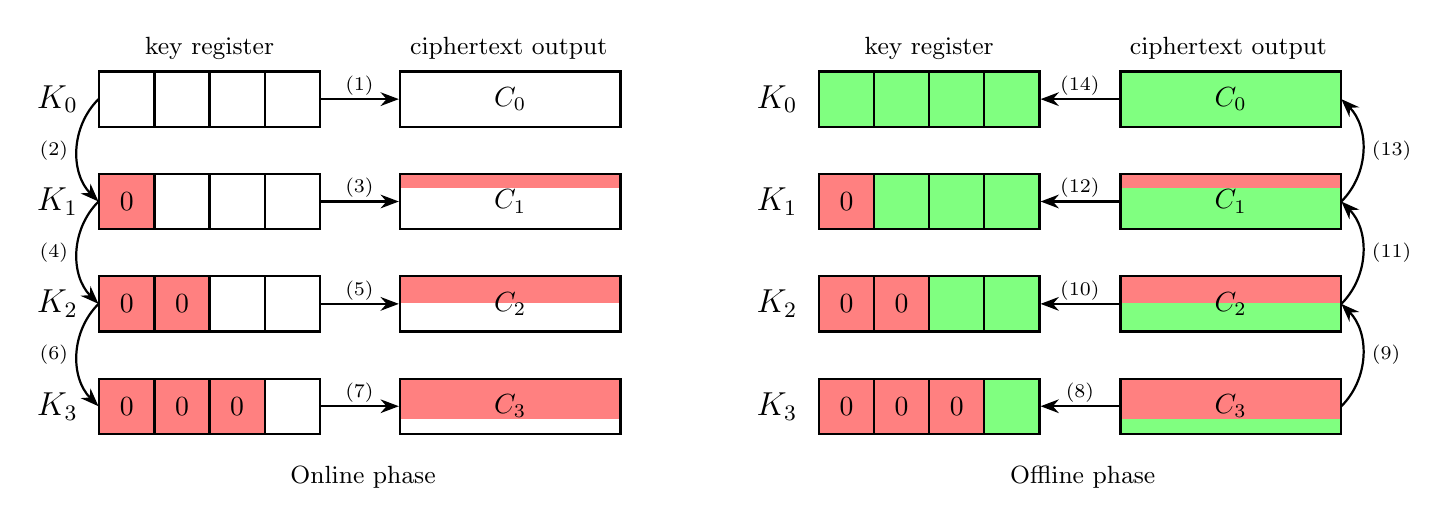
\begin{tikzpicture}[
    box/.style={draw, thick, minimum width=1.2cm, minimum height=0.7cm, anchor=west},
    reg/.style={minimum height=0.7cm, minimum width=0.7*4cm, anchor=west},
    arr/.style={thick,->,>=Stealth},
    lab/.style={anchor=east, font=\bfseries\large},
    subword/.style={draw, thick, minimum height=0.7cm, minimum width=0.7cm, fill=white},
    subwordred/.style={draw, thick, minimum height=0.7cm, minimum width=0.7cm, fill=red!50},
    subwordredhoriz/.style={inner sep=0pt, outer sep=0pt, text height=0.176cm, minimum width=2.8cm, fill=red!50, draw=none},
    subwordgreen/.style={draw, thick, minimum height=0.7cm, minimum width=0.7cm, fill=green!50},
    subwordgreenhoriz/.style={inner sep=0pt, outer sep=0pt, text height=0.176cm, minimum width=2.8cm, fill=green!50, draw=none},
    cyclab/.style={font=\scriptsize, inner sep=1pt}
]

% Phase 1
\foreach \i in {0,1,2,3} {
    \node[lab] (K\i) at (0,-\i*1.3) {$K_{\i}$};
}
\node at (1.55,0.65) [font=\small] {key register};
\node at (1.55+1+0.7*4,0.65) [font=\small] {ciphertext output};

% Key register boxes (phase 1)
\foreach \i in {0,1,2,3} {
    \node[reg] (KR\i) at (0.14,-\i*1.3) {};
    \foreach \j in {0,1,2,3} {
        \ifnum\j<\i
            \node[subwordred] at (0.5+0.7*\j,-\i*1.3) {0};
        \else
            \node[subword] at (0.5+0.7*\j,-\i*1.3) {};
        \fi
    }
}

\foreach \i in {1,2,3} {
            \node[subwordredhoriz, text height=0.175cm*\i] at (5.38,0.35-\i*1.385) {};
}
% Arrow to ciphertext (A)
\foreach \i in {0,1,2,3} {
    \draw[arr] (KR\i.east) -- ++(1,0) node[midway, above=0pt, cyclab] {(\the\numexpr\i*2+1\relax)} node[reg, draw] (C\i) {$C_{\i}$};
}

% Arrow to next register step (B)
\foreach \i in {1,2,3} {
    \draw[
      thick, bend right=45,
      -{Stealth}] (KR\the\numexpr\i-1\relax.west) to node[cyclab, left=0.07cm] {(\the\numexpr\i*2\relax)} (KR\i.west);
  }

% Phase 2 (to the right)
\foreach \i in {0,1,2,3} {
    \node[lab] (K2\i) at (9.14,-\i*1.3) {$K_{\i}$};
}
\node[] at (1.55+9.14,0.65) [font=\small] {key register};
\node at (1.55+1+0.7*4+9.14,0.65) [font=\small] {ciphertext output};

\foreach \i in {0,1,2,3} {
    \node[reg] (K2R\i) at (0.15+9.14,-\i*1.3) {};
    \foreach \j in {0,1,2,3} {
        \ifnum\j<\i
            \node[subwordred] at (0.5+0.7*\j+9.14,-\i*1.3) {0};
        \else
            \node[subwordgreen] at (0.5+0.7*\j+9.14,-\i*1.3) {};
        \fi
    }
}

\foreach \i in {0,1,2,3} {
    \node[subwordgreenhoriz, text height=0.7cm] at (5.38+9.14,-\i*1.3) {};
}
\foreach \i in {1,2,3} {
    \node[subwordredhoriz, text height=0.175cm*\i] at (5.38+9.14,0.35-\i*1.385) {};
}
% Arrow to key register (C)
\foreach \i in {0,1,2,3} {
    \draw[arr, <-] (K2R\i.east) -- ++(1,0) node[midway, above=0pt, cyclab] {(\the\numexpr14-\i*2\relax)} node[reg, draw] (C\i) {$C_{\i}$};
  }

% Arrow to prev register step D)
\foreach \i in {1,2,3} {
    % \draw[
    %   thick, bend right=45, <-,
    %   >={Stealth}] (K2R\the\numexpr\i-1\relax.west) to node[cyclab, left=0.07cm] {(\the\numexpr15-\i*2\relax)} (K2R\i.west);
    \draw[
      thick, bend right=-45, <-,
      >={Stealth}] ($(K2R\the\numexpr\i-1\relax.east) + (3.82cm,0)$) to node[cyclab, right=0.07cm] {(\the\numexpr15-\i*2\relax)} ($(K2R\i.east)+ (3.82cm,0)$);
}
\node at (3.5,-4.8) [font=\small] {Online phase};
\node at (3.5+9.14,-4.8) [font=\small] {Offline phase};

\end{tikzpicture}

  \caption{Diagram of the PKO attack on counterfeit cards, as introduced in~\cite{article3940}.}
  \label{fig:pko}
\end{figure*}

The final key recovery is conducted offline in a staged, reverse-chronological manner, as illustrated by the arrows (9) to (14), with the recovered segments represented in green. The process begins with a brute-force search of the first $2^{28}$ possibilities, corresponding to a key that is 75\% zeroed. Each key candidate is validated by checking if the decrypted nonce conforms to the known mathematical properties of the card's specific LFSR. The following functions demonstrate this validation respectively for ULCG and for cards using the historical MIFARE Classic LFSR: FJ8010 and USCUID-UL.
\begin{lstlisting}[style=customc]
bool valid_lfsr_ulcg(uint64_t x64) {
    x64 = __builtin_bswap64(x64);
    uint16_t x16 = x64 >> 48;
    x16 = x16 << 15 | (x16 >> 1) ^ ((x16 >> 3 ^ x16 >> 4 ^ x16 >> 6) & 1);
    if (x16 != ((x64 >> 32) & 0xFFFF)) return false;
    x16 = x16 << 15 | (x16 >> 1) ^ ((x16 >> 3 ^ x16 >> 4 ^ x16 >> 6) & 1);
    if (x16 != ((x64 >> 16) & 0xFFFF)) return false;
    x16 = x16 << 15 | (x16 >> 1) ^ ((x16 >> 3 ^ x16 >> 4 ^ x16 >> 6) & 1);
    if (x16 != (x64 & 0xFFFF)) return false;
    return true;
}
\end{lstlisting}
\begin{lstlisting}[style=customc]
bool valid_lfsr_mfc(uint64_t x64) {
    x64 = __builtin_bswap64(x64);
    uint16_t x16 = x64 & 0xFFFF;
    for (int i = 0; i < 16; i++) x16 = x16 >> 1 | (x16 ^ x16 >> 2 ^ x16 >> 3 ^ x16 >> 5) << 15;
    if (x16 != ((x64 >> 16) & 0xFFFF)) return false;
    for (int i = 0; i < 16; i++) x16 = x16 >> 1 | (x16 ^ x16 >> 2 ^ x16 >> 3 ^ x16 >> 5) << 15;
    if (x16 != ((x64 >> 32) & 0xFFFF)) return false;
    for (int i = 0; i < 16; i++) x16 = x16 >> 1 | (x16 ^ x16 >> 2 ^ x16 >> 3 ^ x16 >> 5) << 15;
    if (x16 != ((x64 >> 48) & 0xFFFF)) return false;
    return true;
}
\end{lstlisting}

After the first portion of the key is recovered, the attack proceeds to the next segment with a 50\% zeroed key, followed by a 25\% zeroed key, until the entire 112-bit 2TDEA key is reconstructed~\cite{article3940}. The fully recovered key is then written back to the card. This attack methodology has been implemented and made available in tools such as the \texttt{mfulc\_counterfeit\_recovery} script on the Proxmark3, the \texttt{hf mfu ulcg} script on the ChameleonUltra, and the ULCFKey application for the Flipper Zero.

\subsection{Behavioral Comparison of Genuine and Counterfeit Cards}
\label{sec:fingerprint_ulc}
We highlighted a few differences in the previous sections but a deeper analysis is available in Appendix~\ref{app:fingerprint_ulc}, showing the different responses to the same commands when the commands are malformed, misplaced, or don't correspond to standard commands.
This can serve as a basis to fingerprint cards and distinguish genuine MIFARE Ultralight~C cards from counterfeit ones. We integrated this fingerprinting into the Proxmark3 \texttt{hf mfu info} command.
Another method to quickly distinguish genuine and certain counterfeit cards while only using legitimate commands is to measure the response time of the card -- a.k.a. the Frame Delay Time (FDT) -- especially when an authentication is attempted with a purposely wrong key, as the timings differ significantly: $78~{\mu}s$ for the Giantec, $842~{\mu}s$ for the NXP and $3646~{\mu}s$ for the ULCUID-UL variant 1 card.

\section{Impact on MIFARE Ultralight~AES}
\label{sec:ulaes}
The vulnerabilities identified for MIFARE Ultralight~C exhibit comparable implications for MIFARE Ultralight~AES (MF0AES), particularly when deployed without utilizing its integrity protection features such as CMAC and lock bits. Although AES-based authentication provides a cryptographic improvement over Ultralight~C's two-key Triple DES, several key design and implementation similarities expose Ultralight~AES to analogous classes of relay, keyspace reduction, and tearing attacks. Notably, the optional CMAC-based integrity protection in MF0AES --- absent in Ultralight~C --- helps protect the integrity of the communication. However, it only offers partial mitigation and does not fully address all attack vectors, such as relayed tearing involving WRITE commands. Additionally, the protocol has not transitioned away from plaintext communication, leaving memory contents vulnerable to unauthorized readouts post-authentication by sniffing traffic.
The attacks detailed in the next sub-sections greatly depend on the degree of adherence of the integrator to the recommendations expressed in a supplemental application note~\cite{nxp_an13452}, as the MF0AES datasheet~\cite{mf0aes_3r2_2023} alone falls short of proper recommendations.

\subsection{Ultralight~AES: Relay Attack}
\label{sec:aesrelay}

MF0AES remains vulnerable to the relay attack described in Section~\ref{sec:relay} because the protocol design places timing constraints only on the reader's side. The tag remains in an idle state receptive to the reader's response after sending its encrypted challenge, allowing attackers to relay encrypted challenges and responses between genuine readers and tags without challenging timing constraints.

While the optional CMAC mode in Ultralight~AES offers protection against attackers injecting unauthorized commands by enforcing integrity checks, the default configuration of MF0AES has \texttt{SEC\_MSG\_ACT} disabled. In this insecure configuration, a successful relay grants the attacker the ability to issue arbitrary authenticated commands (although write commands may be limited based on lock bits, which are unset by default). With CMAC enabled, the protocol remains susceptible to relayed tearing attacks --- depending on reader timing constraints --- by exploiting interruptions to genuine WRITE commands.

\subsection{Ultralight~AES: Keyspace Reduction}
\label{sec:aes_ks_reduc}
MIFARE Ultralight~AES stores \texttt{DataProtKey} --- a 128-bit AES key --- across four consecutive memory pages, mirroring the design of Ultralight~C. 

Besides \texttt{DataProtKey}, MIFARE Ultralight~AES stores a second 128-bit key called \texttt{UIDRetrKey}. This key is of more limited interest because it is only used to access the real UID of a tag that has the Random ID (RID) activated. Once the UID is known, a reader can proceed with its KDF to compute the diversified key of a given tag. Nevertheless, by nature, \texttt{UIDRetrKey} is a static key shared between all tags and readers of the system and is therefore harder to protect.

Assuming the pages of the targeted key are not write-protected by the corresponding lock bits (\texttt{LOCK\_AES\_KEY0} or \texttt{LOCK\_AES\_KEY1}), the partial key overwrite technique remains applicable due to the absence of enforced atomicity during WRITE operations. This is accomplished either through plaintext command injection during a relay attack when CMAC is inactive, when \texttt{AUTH0} is directly writable, or when \texttt{AUTH0} is set to a value greater or equal to 51~(\texttt{0x33}) for \texttt{DataProtKey} or 55~(\texttt{0x37}) for \texttt{UIDRetrKey}. By overwriting three of the four key pages with a known value (e.g., zeros), the attacker reduces the complexity of an online brute-force attack against the remaining key material from \(2^{128}\) to \(2^{32}\). While \(2^{32}\) is still substantial, it falls within the bounds of what is practically achievable in an online attack scenario. Recovering the full 128-bit AES key using this method requires combining the results of four separate online attacks against different tags, with a total of \(2^{33}\) authentication attempts on average, assuming a static key is shared across the deployment --- which is always true for \texttt{UIDRetrKey}. In contrast, if Random ID and \texttt{UIDRetrKey} are set, it is likely that \texttt{DataProtKey} is diversified.

\subsection{Ultralight~AES: Tearing}
\label{sec:aes_tearing}
The $2^{32}$ keyspace for a single segment can be further reduced through EEPROM tearing if more than 4 tags sharing the same key are available. Attacking one key segment will require attacking the same segment of the other key as well, so \texttt{AUTH0} must have a sufficient value.

This unexpected relationship deserves an explanation.
After attempting to zero a segment by tearing after the erase phase, we could not authenticate with the corresponding segment of the key set to zero. We then hypothesized that a mask was used when the actual key is stored in the EEPROM, potentially as a countermeasure against side-channel attacks.
We started with a zero-key segment, then began tearing operations to progressively erase the segment. Whenever we could not authenticate with the zero key, we tested key candidates with a small Hamming distance, i.e. flipping just one or two bits. Every time we could recover the new key value, we continued tearing and recovering more bits, until the value discernibly stabilized between the erase and the write operations.
Once the procedure was repeated on the four segments, we could recover the entire 128-bit mask. The mask can be validated by tearing the four segments and attempting to authenticate using the mask as a key. What is stored is mask $\oplus$ key so if key=mask, what is stored is mask $\oplus$ mask = 0, which corresponds to our erased segments in the EEPROM.
Once automated, the entire 128-bit mask recovery process takes 7 minutes on average. 

The recovered mask is unique to each tag but is shared between \texttt{DataProtKey} and \texttt{UIDRetrKey}.
Despite this mask, we can apply almost the same strategy as Ultralight~C. For each tag, we overwrite \texttt{UIDRetrKey} -- or inversely \texttt{DataProtKey} if we want to recover \texttt{UIDRetrKey} -- with our tearing tests to extract the mask. Once the mask of the tag is identified, we can attack a few bits of \texttt{DataProtKey}, knowing that we have to find the masked key candidates with a small Hamming distance to the mask. Finally, we compute the bitwise XOR of the masked key with the mask itself to yield the recovered bits of the key. It is critical to note that each recovered bit is the logical inverse of the corresponding bit in the mask. This property must be systematically accounted for when aggregating the partial key information obtained from multiple tags.

As the key segments are 32 bits long instead of 28, there are slightly more key candidates to test: 5489 with a Hamming distance $HW\leq 3$ and 529 for $HW\leq 2$, which is enough in practice if tags are easily available.

Tearing timing data can be calibrated by experimenting on unlocked user memory pages. This calibration helps to estimate the parameters for a blind tearing attempt on the key pages. We observed that the timings are not the same across the whole block range and we advise to use blocks 56-59 (RFU)\footnote{If you are willing to test other RFU, beware that page 46 is write-once and pages 43--44 cannot be modified.} as reference.

\subsection{Ultralight~AES: Tearing Optimizations}
\label{sec:aes_tearing2}

As established in Section~\ref{sec:envweak}, environmental factors such as distance and temperature can be manipulated to influence the outcome of tearing attempts and key readings during the authentication phase.
To test these bit revival techniques on Ultralight~AES keys, we limit brute-force attempts to candidates at a Hamming distance $\leq 2$ to maintain efficiency.
The procedure begins with a series of tearing operations on a target segment until approximately 2 bits are recovered (see Section~\ref{sec:aes_tearing}).
Subsequently, we perform continuous authentication attempts using the partially recovered key. Upon authentication failure, a rapid brute-force search is triggered for all candidates at $HD \leq 2$. Successful candidates are logged as updated partial keys. To maximize bitflip probability, we apply external thermal stress to the card. It should be noted that stochastic bitflips were observed even at ambient temperatures.
Continuous brute-force of keys at HD $\leq 2$ is critical because bitflips are transient; a single-pass test might fail to capture an unstable bit if its state fluctuates during the measurement window.
Initial testing on eight segments --- each containing an unmasked 32-bit key with $HW=16$ --- resulted in an average recovery of 5.875 bits per segment.

We can further improve the attack by considering the late-erasing bits as introduced in Section~\ref{sec:lateerase}, provided erroneous guesses are accounted for.
To evaluate the effectiveness of this technique, we tested three distinct recovery strategies based on bitflip events across the same eight segments:
\begin{itemize}
    \item \textbf{Conservative Strategy:} By targeting only those bits that remained unflipped during characterization (while all recovered bits had already transitioned), we assume these bits represent a $0$ in EEPROM. This yielded an average of 0.875 additional bits per segment, without error.
    \item \textbf{Aggressive Strategy:} We assume any bit that remained unflipped when the \emph{first} of our recovered key bits transitioned is $0$. This increased the average recovery to 8 bits per segment but introduced 1.6 erroneous bits, significantly increasing the complexity of the final key search.
    \item \textbf{Filtered Strategy:} By applying a crude filter --- specifically skipping the first two flip events following the initial recovered bit transition --- the average recovery rate adjusted to 6.75 bits per segment with a reduced error rate of 0.875 bits.
\end{itemize}
Integrating the filtered strategy allows for the recovery of 12.625 bits per segment on average, including 0.875 erroneous bits within a subset of 6.75 bits.
This means that on average, from a single card, we can extract 50.5 bits of the AES key, comprising 3.5 erroneous bits located among 27 bits.
Further refinements may be possible by iterating the characterization phase, and measuring the precise number of tearing events between bitflips to weight the probability of bit correctness. We can also challenge the assumption that the slowest bits to be erased are the first ones to be revived by heating, by conducting a heat-recovery characterization of the suspected $0$ bits, along with the already recovered ones, to verify if they reappear.

\subsection{Ultralight~AES: Reader Nonces, Online Attack Enhancements}
\label{sec:aes_readernonce}
    
Nonce pairs can be collected from the reader during interactions. Their effectiveness in attacks varies between Ultralight~AES and Ultralight~C. Due to the larger keyspace of AES-128, offline brute-force key recovery using collected nonces is generally limited to a single page ($2^{32}$). Recovering half of the key (64 bits) using reader nonces is computationally prohibitive, unlike the $2^{56}$ complexity for a similar attack against 2TDEA. Therefore, the minimum number of tags recommended for recovering a static key on Ultralight~AES is three.

Optimizations made to the online brute-force attack can be directly applied to Ultralight~AES as well. The key guessing process can be accelerated by issuing the \texttt{WUPA} command to reinitialize the tag after a failed authentication, avoiding the need to cycle the RF field. In addition, Ultralight~AES supports the same READ~0 optimization technique identified in Ultralight~C, permitting direct transition to the ACTIVE state. These optimizations support practical online brute-force rates similar to Ultralight~C (a hundred attempts per second), even on resource-constrained attack hardware. This further underscores the practical feasibility of these attacks in the absence of mitigations.

A significant difference in Ultralight~AES is the introduction of an optional authentication attempt counter, controlled by the \texttt{AUTH\_LIM} configuration bytes. If enabled and properly locked (\texttt{LOCK\_USR\_CFG}), this feature effectively prevents online brute-force attacks. However, if \texttt{AUTH\_LIM} is configurable via user memory and that memory is not locked, an attacker gaining authenticated plaintext access (via the relay attack or weak configuration) could potentially overwrite \texttt{AUTH\_LIM} to zero, disabling the counter and permitting unlimited brute-force attempts. Furthermore, while the TRNG in genuine NXP Ultralight~AES ICs appears to be sufficiently random, the state machine permits nested authentications with the same valid key. As a result, its output can be analyzed more easily than with Ultralight~C.

Overall, while Ultralight~AES introduces cryptographic improvements over Ultralight~C, inadequate deployment practices -- such as failure to utilize CMAC and incomplete lock-bit configuration -- permit similar exploitation methods. Despite cryptographic advancements, Ultralight~AES deployments with static keys risk compromise through relay attacks, partial key overwrites, tearing attacks, and optimized online attacks if integrators do not strictly enforce available protections.

\subsection{Ultralight~AES: Protocol Oddity}
\label{sec:aes_oddity}
Ultralight~C mutual authentication protocol was presented in Section~\ref{sec:ulc_auth}.
Ultralight~AES shares almost the same protocol, exchanging \textit{ek(RndB)} then \textit{ek(RndA $||$ RndB')} then \textit{ek(RndA')}, but with the following differences.
\begin{itemize}
    \item 3DES-CBC is replaced by AES-128-CBC ;
    \item The nonces are extended to the larger cipher block size, from 8 to 16 bytes ;
    \item The IV is always null, instead of being chained from the previous encrypted block.
\end{itemize}

We don't know why the IV is not chained anymore (the DESFire protocol with AES still chains IVs) but this has an impact when the reader does not generate good randoms.
With an Ultralight~C, if the reader random \textit{RndA} can be zeroed (or made constant), a classic replay attack can be done by sniffing a transaction between the reader and a legitimate tag, then replaying the tag messages.
But with an Ultralight~AES, if the reader random can be zeroed (or made as a stream of constant bytes), one can immediately pretend to have a valid tag, simply by replaying the first half of the reader's message, as \textit{ek(RndA)==ek(RndA')}.
This issue could only affect readers based on low-cost microcontrollers with a poor source of entropy. For instance, a reader relying on a floating ADC input that could be grounded, saturated, or --- if sampled byte per byte --- rendered constant.

\section{Impact on NTAG~223~DNA and NTAG~224~DNA}
\label{sec:ntag22x}

\begin{figure*}[!b]
  \centering
  \input{suncmacpko}
  \caption{Diagram of the PKO attack on NTAG~22x SUNCMAC.}
  \label{fig:suncmacpko}
\end{figure*}

The public security target documentation for Ultralight~AES~\cite{mf0aes_st_1r1_2022} reveals that the same IC architecture is used for the NTAG~22x~DNA (NT2H2xy1G)~\cite{nt2h2331g0_3r1_2023, nt2h2421g0_3r2_2023} and NTAG~22x~DNA StatusDetect (NT2H2xy1S)~\cite{nt2h2331s0_3r1_2023, nt2h2421s0_3r2_2023} variants.
While NTAG~224~DNA offers the same 3-pass mutual authentication protocol as Ultralight~AES, NTAG~223~DNA uses password authentication similar to Ultralight~EV1.
Neither NTAG~22x~DNA products offer CMAC integrity protection over communicated frames or the \texttt{UIDRetrKey} seen in Ultralight~AES. NTAG~22x~DNA also lacks anti-tearing protection for general configuration bytes, similar to Ultralight~C and Ultralight~AES.
However, both are NFC Forum Type 2 compatible and offer dynamic NFC Data Exchange Format (NDEF) message support -- for example, to include a counter -- protected by a Secure Unique NFC (SUN) message authentication based on a configurable AES-128 CMAC key, the \texttt{SUNCMAC\_KEY}. Such messages are referred to as SUN messages.
This section highlights the similarities and differences between the NTAG~22x~DNA and Ultralight~AES attack vectors.

The NTAG~22x~DNA series is intended for different use cases from those targeted by Ultralight~AES.
Nevertheless, we may see in the future an adoption of NTAG~224~DNA in the hospitality industry, leveraging its NFC Forum compatibility to bring the enriched experience promised by MIFARE Hospitality in 2019.

At the time of writing, we could only obtain a few NTAG~223~DNA StatusDetect samples but no NTAG~224~DNA. Therefore, our interpretations on NTAG~224~DNA should be treated as preliminary. When a feature of NTAG~224~DNA appears identical to a feature of Ultralight~AES, we consider that its implementation is identical to the one observed in Ultralight~AES.

\subsection{NTAG~22x~DNA: Relay Attack}

The NTAG~22x~DNA series is also vulnerable to relay attacks due to the absence of PICC timing constraints. Moreover, they do not feature a CMAC mode and, as a result, their communication remains unprotected against traffic manipulation and command injection.

NTAG~223~DNA only offers password authentication, which should never be performed in a hostile environment, as sniffing or relaying would immediately reveal the password.

\subsection{NTAG~224~DNA: \texttt{AES\_KEY} Keyspace Reduction}

NTAG~224~DNA stores its 3-pass authentication key \texttt{AES\_KEY} across memory pages 64--67, analogous to Ultralight~AES storing its \texttt{DataProtKey} in pages 48--51.

Assuming that the pages that store \texttt{AES\_KEY} are not write-protected by the \texttt{LOCK\_AES\_KEY} lock bit configuration, the partial key overwrite technique of Section~\ref{sec:aes_ks_reduc} remains applicable under the same conditions as Ultralight~AES. In such cases, three quarters of the key can be overwritten, allowing an attacker to reduce the complexity of an online brute-force attack against the remaining key material from \(2^{128}\) to \(2^{32}\).
By targeting distinct quarters of the key across multiple tags, an attacker can combine the recovered portions to reconstruct the complete 128-bit AES key with an average of \(2^{33}\) authentication attempts, assuming the deployment uses a static key.

\subsection{NTAG~22x~DNA: \texttt{SUNCMAC\_KEY} Keyspace Reduction}
The NTAG~223~DNA and NTAG~224~DNA implement an AES-128 key, \texttt{SUNCMAC\_KEY}, for Secure Unique NFC (SUN) CMAC computation. This key is likewise susceptible to the partial key overwrite technique, if permitted by the \texttt{LOCK\_SUNCMAC\_KEY} lock bit configuration.
However, the SUN message and its CMAC itself introduce an additional element to the attack. Indeed, this key does not need to be tested against the authentication protocol, but rather against the SUN messages that are protected by it. The SUNCMAC can be viewed as an unauthenticated oracle that produces distinct outputs when the key is modified. Once the key is partially overwritten, we only need the tag to generate one SUN message and collect it with its 64-bit authentication tag to brute-force the 32-bit \texttt{SUNCMAC\_KEY} segment offline. This requires the ASCII mirror functionality to be activated and properly configured, but the NFC counter does not need to be enabled.
Therefore, we can progressively erase the key, collect one SUN message at each step, then brute-force at each step the $2^{32}$ \texttt{SUNCMAC\_KEY} candidates offline, beginning with the 75\% overwritten value and reconstructing the original key in reverse. The strategy, shown in Figure~\ref{fig:suncmacpko}, is very similar to the one presented in Figure~\ref{fig:pko}. This technique requires a single tag, which implies that it is effective even if \texttt{SUNCMAC\_KEY} is diversified.

\subsection{NTAG~22x~DNA: Tearing}
\label{sec:ntag22x_tear}

Based on our experiments on NTAG~223~DNA, we could determine that the \texttt{SUNCMAC\_KEY} is stored in EEPROM after a bitwise XOR with a mask value, diversified for each sample, which mirrors the properties of Ultralight~AES.

Tear-off attacks accelerate the recovery of the \texttt{SUNCMAC\_KEY} through a two-stage methodology. The initial data acquisition stage involves the systematic collection of SUN messages generated as the \texttt{SUNCMAC\_KEY} undergoes tearing towards an unknown 128-bit mask: first from the target \texttt{SUNCMAC\_KEY} and next from a known key. The resulting corpus of SUN messages facilitates a subsequent offline brute-force search that reconstructs first the mask, and then the entire \texttt{SUNCMAC\_KEY}, achieving key recovery from a single tag in less than a minute.

The process pictured in Figure~\ref{fig:suncmactearpko} is as follows.
\begin{itemize}
    \item Ensure ASCII mirroring is enabled (\texttt{MIRROR\_EN} is set to 1 and \texttt{MIRROR\_PAGE} is between \texttt{0x04} and \texttt{0x1B}), writing on key blocks is allowed, and, if possible, disable the NFC counter (and live Capacitive Tag Tamper (CTT) measures on StatusDetect variants) ;
    \item Target one \texttt{SUNCMAC\_KEY} segment. Collect SUN messages while progressively tearing the segment from the \texttt{SUNCMAC\_KEY} to the mask value. Repeat for the other segments. The steps are illustrated by the arrows (1) to (9), with the unknown mask segments represented in blue ;
    \item Write zeroes to the 4 segments over the mask segments, one at the time, and collect the SUN message corresponding to keys with 75\%, 50\% and 25\% of the mask. Cf arrows (10) and (11). Zeroed segments are represented in red ;
    \item Process as in the second step: target one segment, tear progressively towards the mask value while collecting SUN messages. The SUN messages collected in the previous step allow quick identification when the tearing operations have reached the mask value. Repeat for the other segments. Cf arrows (12) to (19) ;
    \item Now starts the offline phase, which can run in parallel of the previous step. As we start from a known key=0, we can recover the keys of each intermediate SUNCMAC, always at a small Hamming distance from the previous key, following the arrows (20) to (27). Recovered mask segments appear in yellow. The brute-force being offline, a ``small Hamming distance'' can still be relatively large for little cost. At the end the full mask will be recovered ;
    \item Now that the mask is known, the SUN messages collected at the second step can be processed in reverse, finding intermediate keys at small Hamming distance from the mask value up to the \texttt{SUNCMAC\_KEY} value, as illustrated by arrows (28) to (35) with recovered key segments represented in green.
\end{itemize}

\begin{figure*}[!htb]
  \centering
  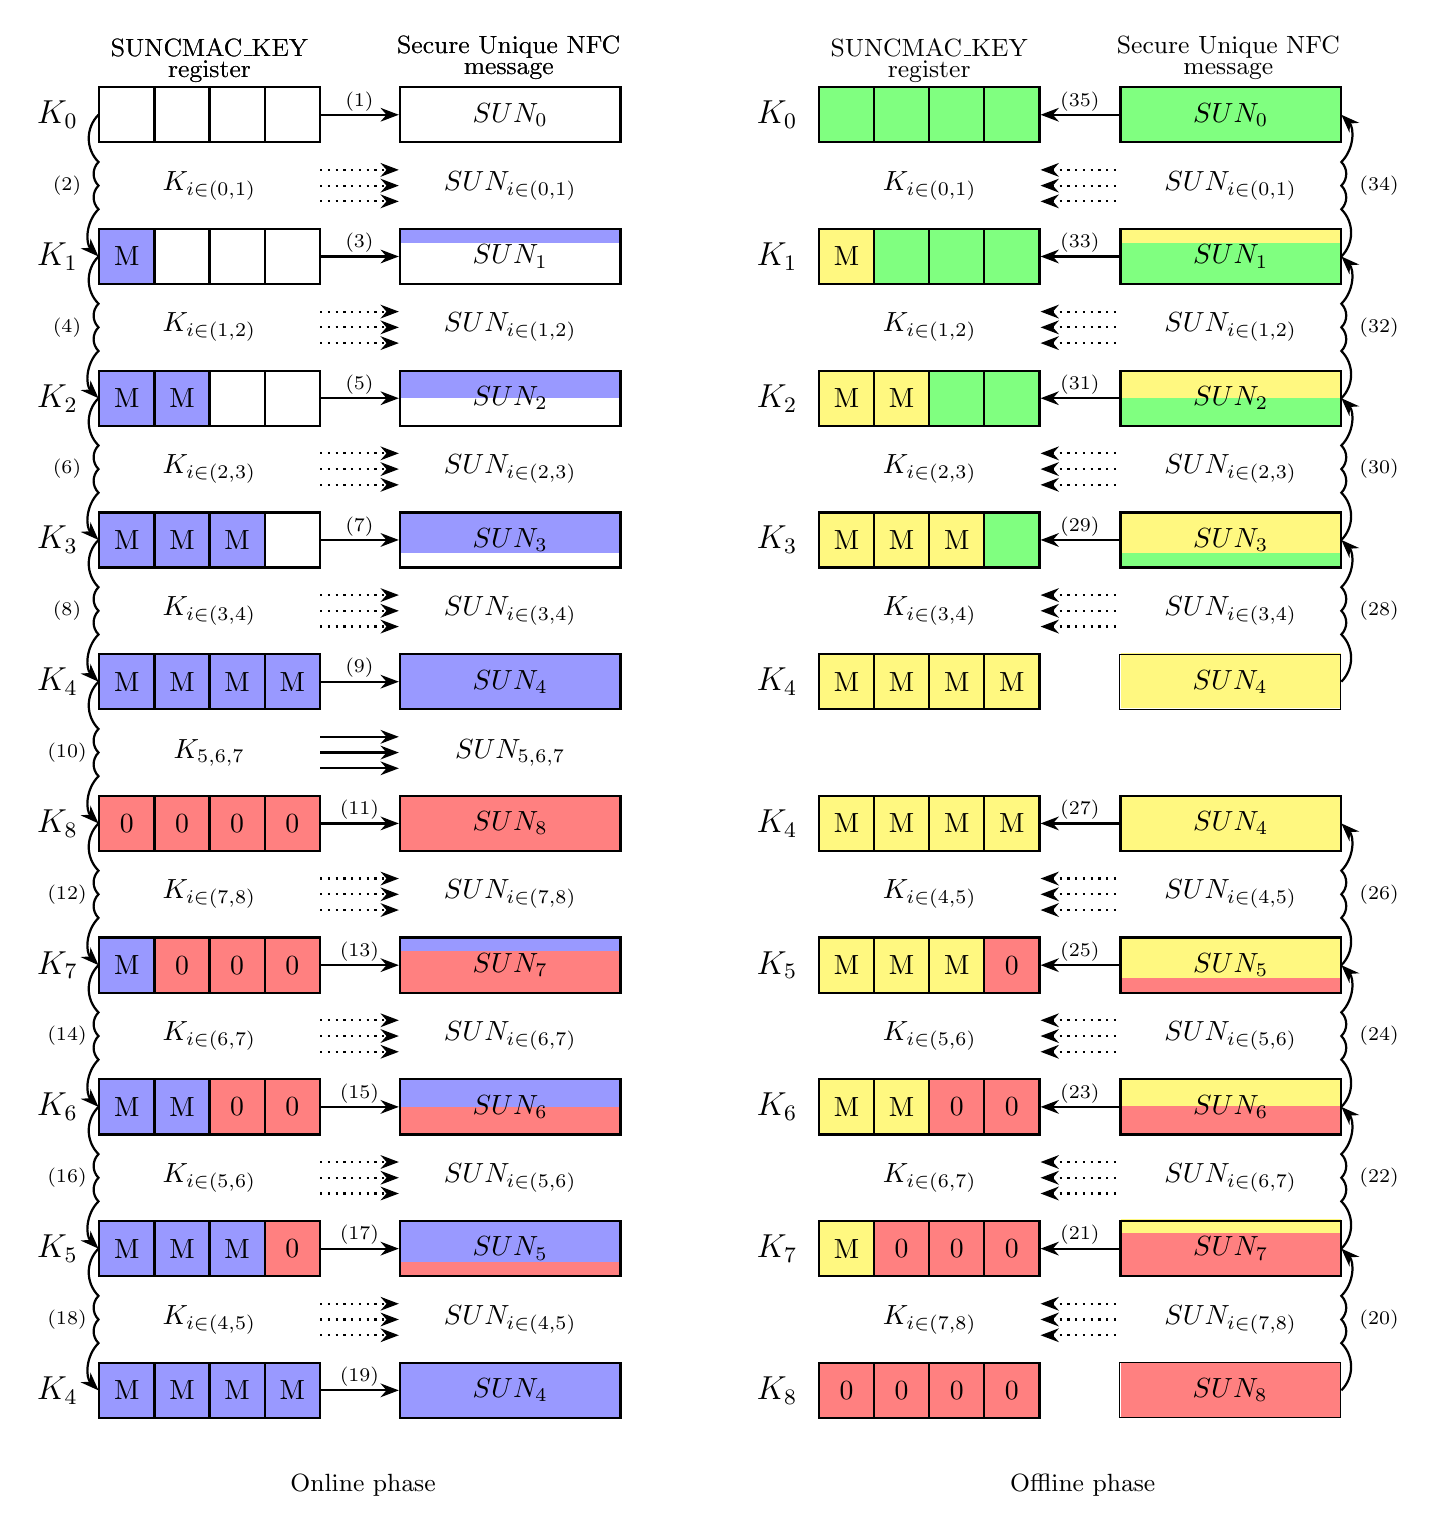
\begin{tikzpicture}[
    box/.style={draw, thick, minimum width=1.2cm, minimum height=0.7cm, anchor=west},
    reg/.style={minimum height=0.7cm, minimum width=0.7*4cm, anchor=west},
    arr/.style={thick,->,>=Stealth},
    lab/.style={anchor=east, font=\bfseries\large},
    subword/.style={draw, thick, minimum height=0.7cm, minimum width=0.7cm, fill=white},
    subwordred/.style={draw, thick, minimum height=0.7cm, minimum width=0.7cm, fill=red!50},
    subwordredhoriz/.style={inner sep=0pt, outer sep=0pt, text height=0.176cm, minimum width=2.8cm, fill=red!50, draw=none},
    subwordblue/.style={draw, thick, minimum height=0.7cm, minimum width=0.7cm, fill=blue!40},
    subwordbluehoriz/.style={inner sep=0pt, outer sep=0pt, text height=0.176cm, minimum width=2.8cm, fill=blue!40, draw=none},
    subwordgreen/.style={draw, thick, minimum height=0.7cm, minimum width=0.7cm, fill=green!50},
    subwordgreenhoriz/.style={inner sep=0pt, outer sep=0pt, text height=0.176cm, minimum width=2.8cm, fill=green!50, draw=none},
    subwordyellow/.style={draw, thick, minimum height=0.7cm, minimum width=0.7cm, fill=yellow!50},
    subwordyellowhoriz/.style={inner sep=0pt, outer sep=0pt, text height=0.176cm, minimum width=2.8cm, fill=yellow!50, draw=none},
    cyclab/.style={font=\scriptsize, inner sep=1pt}
]

% Phase 1
\foreach \i in {0,1,2,3,4} {
    \node[lab] (K\i) at (0,-\i*1.8) {$K_{\i}$};
}
\node at (1.55,0.85) [font=\small] {SUNCMAC\_KEY};
\node at (1.55,0.55) [font=\small] {register};
\node at (1.55+1+0.7*4,0.85) [font=\small] {Secure Unique NFC};
\node at (1.55+1+0.7*4,0.55) [font=\small] {message};

% Key register boxes (phase 1)
\foreach \i in {0,1,2,3,4} {
    \node[reg] (KR\i) at (0.14,-\i*1.8) {};
    \foreach \j in {0,1,2,3} {
        \ifnum\j<\i
            \node[subwordblue] at (0.5+0.7*\j,-\i*1.8) {M};
        \else
            \node[subword] at (0.5+0.7*\j,-\i*1.8) {};
        \fi
    }
}
% Tear nodes (invisible)
\foreach \i in {0,1,2,3,4} {
    \node[reg] (KRT\i) at (0.14,-\i*1.8-0.9) {};
}

\foreach \i in {1,2,3,4} {
            \node[subwordbluehoriz, text height=0.175cm*\i] at (5.38,0.35-\i*1.885) {};
}
% Arrow to ciphertext (A)
\foreach \i in {0,1,2,3,4} {
    \draw[arr] (KR\i.east) -- ++(1,0) node[midway, above=0pt, cyclab] {(\the\numexpr\i*2+1\relax)} node[reg, draw] (SUN\i) {$SUN_{\i}$};
}
% Tear steps
\foreach \i in {0,1,2,3} {
    \draw[arr, dotted] (KRT\i.east) -- ++(1,0) node[midway, above=0pt, cyclab] {} node[reg] (SUN\i) {$SUN_{i \in (\the\numexpr\i\relax, \the\numexpr\i+1\relax)}$};
    \draw[arr, dotted] ($(KRT\i.east) + (0,0.2)$) -- ++(1,0) node[midway, above=0pt, cyclab] {};
    \draw[arr, dotted] ($(KRT\i.east) + (0,-0.2)$) -- ++(1,0) node[midway, above=0pt, cyclab] {};
}
\draw[arr] (KRT4.east) -- ++(1,0) node[midway, above=0pt, cyclab] {} node[reg] (SUN4) {$SUN_{5,6,7}$};
\draw[arr] ($(KRT4.east) + (0,0.2)$) -- ++(1,0) node[midway, above=0pt, cyclab] {};
\draw[arr] ($(KRT4.east) + (0,-0.2)$) -- ++(1,0) node[midway, above=0pt, cyclab] {};

% Arrow to next register step (B)
\foreach \i in {1,2,3,4} {
    \draw[
      thick, bend right=45, -{Stealth}] (KR\the\numexpr\i-1\relax.west)
      to[thick, bend right=45, -{Stealth}] ++(0,-0.6) 
      to[thick, bend right=45, -{Stealth}] ++(0,-0.3) 
      to[thick, bend right=45, -{Stealth}] ++(0,-0.3) 
      to node[cyclab, left=0.07cm] {} (KR\i.west);
    \node[cyclab] at ($(KR\the\numexpr\i-1\relax.west)!0.5!(KR\i.west) + (-0.4,0)$) {(\the\numexpr\i*2\relax)};
    \node[] at ($(KR\the\numexpr\i-1\relax)!0.5!(KR\i)$) {$K_{i \in (\the\numexpr\i-1\relax, \the\numexpr\i\relax)}$};
}
% Phase 1 bis
\foreach \i in {5,6,7,8} {
    \node[lab] (K\i) at (0,-13*1.8+\i*1.8) {$K_{\i}$};
}
\foreach \i in {9} {
    \node[lab] (K\i) at (0,-\i*1.8) {$K_4$};
}

\node at (1.55,0.85) [font=\small] {SUNCMAC\_KEY};
\node at (1.55,0.55) [font=\small] {register};
\node at (1.55+1+0.7*4,0.85) [font=\small] {Secure Unique NFC};
\node at (1.55+1+0.7*4,0.55) [font=\small] {message};

% Key register boxes (phase 1 bis)
\foreach \i in {5,6,7,8,9} {
    \node[reg] (KR\i) at (0.14,-14*1.8+\i*1.8) {};
    \foreach \j in {0,1,2,3} {
        \ifnum\j<\the\numexpr\i-5\relax
            \node[subwordblue] at (0.5+0.7*\j,-\i*1.8) {M};
        \else
            \node[subwordred] at (0.5+0.7*\j,-\i*1.8) {0};
        \fi
    }
}

\draw[
    thick, bend right=45, -{Stealth}] (KR4.west)
    to[thick, bend right=45, -{Stealth}] ++(0,-0.6) 
    to[thick, bend right=45, -{Stealth}] ++(0,-0.3) 
    to[thick, bend right=45, -{Stealth}] ++(0,-0.3) 
    to node[cyclab, left=0.07cm] {} (KR9.west);
\node[cyclab] at ($(KR4.west)!0.5!(KR9.west) + (-0.4,0)$) {(10)};
\node[] at ($(KR4)!0.5!(KR9)$) {$K_{5,6,7}$};

% Tear nodes (invisible)
\foreach \i in {5,6,7,8} {
    \node[reg] (KRT\i) at (0.14,-13*1.8+\i*1.8-0.9) {};
}

\foreach \i in {5,6,7,8} {
    \node[subwordredhoriz, text height=0.7cm] at (5.38,-\i*1.8) {};
}
\foreach \i in {1,2,3,4} {
    \node[subwordbluehoriz, text height=0.175cm*\i] at (5.38,0.35-\i*1.885-5*1.8) {};
}
% Arrow to ciphertext (A)
\foreach \i in {5,6,7,8,9} {
    \draw[arr] (KR\i.east) -- ++(1,0) node[midway, above=0pt, cyclab] {(\the\numexpr29-\i*2\relax)} node[reg, draw] (SUN\i) {$SUN_{\the\numexpr\i-1\relax}$};
}

% Tear steps
\foreach \i in {5,6,7,8} {
    \draw[arr, dotted] (KRT\i.east) -- ++(1,0) node[midway, above=0pt, cyclab] {} node[reg] (SUN\i) {$SUN_{i \in (\the\numexpr\i-1\relax, \the\numexpr\i\relax)}$};
    \draw[arr, dotted] ($(KRT\i.east) + (0,0.2)$) -- ++(1,0) node[midway, above=0pt, cyclab] {};
    \draw[arr, dotted] ($(KRT\i.east) + (0,-0.2)$) -- ++(1,0) node[midway, above=0pt, cyclab] {};
}

% Arrow to next register step (B)
\foreach \i in {6,7,8,9} {
    \draw[
      thick, bend right=45, -{Stealth}] (KR\the\numexpr\i\relax.west)
      to[thick, bend right=45, -{Stealth}] ++(0,-0.6) 
      to[thick, bend right=45, -{Stealth}] ++(0,-0.3) 
      to[thick, bend right=45, -{Stealth}] ++(0,-0.3) 
      to node[cyclab, left=0.07cm] {} (KR\the\numexpr\i-1\relax.west);
    \node[cyclab] at ($(KR\the\numexpr\i-1\relax.west)!0.5!(KR\i.west) + (-0.4,0)$) {(\the\numexpr30-\i*2\relax)};
    \node[] at ($(KR\the\numexpr\i-1\relax)!0.5!(KR\i)$) {$K_{i \in (\the\numexpr\i-2\relax, \the\numexpr\i-1\relax)}$};
}


% Phase 2 (to the right)
\foreach \i in {0,1,2,3,4} {
    \node[lab] (K2\i) at (9.14,-\i*1.8) {$K_{\i}$};
}
\node at (1.55+9.14,0.85) [font=\small] {SUNCMAC\_KEY};
\node at (1.55+9.14,0.55) [font=\small] {register};
\node at (1.55+1+0.7*4+9.14,0.85) [font=\small] {Secure Unique NFC};
\node at (1.55+1+0.7*4+9.14,0.55) [font=\small] {message};

\foreach \i in {0,1,2,3,4} {
    \node[reg] (K2R\i) at (0.15+9.14,-\i*1.8) {};
    \foreach \j in {0,1,2,3} {
        \ifnum\j<\i
            \node[subwordyellow] at (0.5+0.7*\j+9.14,-\i*1.8) {M};
        \else
            \node[subwordgreen] at (0.5+0.7*\j+9.14,-\i*1.8) {};
        \fi
    }
}
% Tear nodes (invisible)
\foreach \i in {0,1,2,3,4} {
    \node[reg] (K2RT\i) at (0.15+9.14,-\i*1.8-0.9) {};
}

\foreach \i in {0,1,2,3} {
    \node[subwordgreenhoriz, text height=0.7cm] at (5.38+9.14,-\i*1.8) {};
}
\foreach \i in {1,2,3,4} {
    \node[subwordyellowhoriz, text height=0.175cm*\i] at (5.38+9.14,0.35-\i*1.885) {};
}
% Arrow to key register (C)
\foreach \i in {0,1,2,3} {
    \draw[arr, <-] (K2R\i.east) -- ++(1,0) node[midway, above=0pt, cyclab] {(\the\numexpr35-\i*2\relax)} node[reg, draw] (SUN\i) {$SUN_{\i}$};
}
\foreach \i in {4} {
    \node[reg, draw] (SUN\i) at ($(K2R\i.east) + (1,0)$) {$SUN_{\i}$};
}
% Tear steps
\foreach \i in {0,1,2,3} {
    \draw[arr, <-, dotted] (K2RT\i.east) -- ++(1,0) node[midway, above=0pt, cyclab] {} node[reg] (SUN\i) {$SUN_{i \in (\the\numexpr\i\relax, \the\numexpr\i+1\relax)}$};
    \draw[arr, <-, dotted] ($(K2RT\i.east) + (0,0.2)$) -- ++(1,0) node[midway, above=0pt, cyclab] {};
    \draw[arr, <-, dotted] ($(K2RT\i.east) + (0,-0.2)$) -- ++(1,0) node[midway, above=0pt, cyclab] {};
}

% Arrow to prev register step D)
\foreach \i in {1,2,3,4} {
    % \draw[
    %   thick, bend right=45, <-,
    %   >={Stealth}] (K2R\the\numexpr\i-1\relax.west) to node[cyclab, left=0.07cm] {(\the\numexpr15-\i*2\relax)} (K2R\i.west);
    \draw[
      thick, bend right=-45, <-,
      >={Stealth}] ($(K2R\the\numexpr\i-1\relax.east) + (3.82cm,0)$)
      to[thick, bend right=-45, >={Stealth}] ++(0,-0.6) 
      to[thick, bend right=-45, >={Stealth}] ++(0,-0.3) 
      to[thick, bend right=-45, >={Stealth}] ++(0,-0.3) 
      to node[cyclab, right=0.07cm] {} ($(K2R\i.east)+ (3.82cm,0)$);
    \node[cyclab] at ($(K2R\the\numexpr\i-1\relax.east)!0.5!(K2R\i.east) + (4.3,0)$) {(\the\numexpr36-\i*2\relax)};
    \node[] at ($(K2R\the\numexpr\i-1\relax)!0.5!(K2R\i)$) {$K_{i \in (\the\numexpr\i-1\relax, \the\numexpr\i\relax)}$};
}


% Phase 2 bis

\foreach \i in {5,6,7,8,9} {
    \node[lab] (K2\i) at (9.14,-\i*1.8) {$K_{\the\numexpr\i-1\relax}$};
}

% Tear nodes (invisible)
\foreach \i in {5,6,7,8,9} {
    \node[reg] (K2RT\i) at (0.15+9.14,-\i*1.8-0.9) {};
}

\foreach \i in {5,6,7,8,9} {
    \node[reg] (K2R\i) at (0.15+9.14,-14*1.8+\i*1.8) {};
    \foreach \j in {0,1,2,3} {
        \ifnum\j<\the\numexpr\i-5\relax
            \node[subwordyellow] at (0.5+0.7*\j+9.14,-14*1.8+\i*1.8) {M};
        \else
            \node[subwordred] at (0.5+0.7*\j+9.14,-14*1.8+\i*1.8) {0};
        \fi
    }
}

\foreach \i in {5,6,7,8,9} {
    \node[subwordredhoriz, text height=0.7cm] at (5.38+9.14,-14*1.8+\i*1.8) {};
}
\foreach \i in {6,7,8,9} {
    \node[subwordyellowhoriz, text height=0.175cm*\i-5*0.175cm] at (5.38+9.14,0.35+\i*1.7055-24.7) {};
}
% Arrow to key register (C)
\foreach \i in {5} {
    \node[reg, draw] (SUN\i) at ($(K2R\i.east) + (1,0)$) {$SUN_{\the\numexpr13-\i\relax}$};
}
\foreach \i in {6,7,8,9} {
    \draw[arr, <-] (K2R\i.east) -- ++(1,0) node[midway, above=0pt, cyclab] {(\the\numexpr9+\i*2\relax)} node[reg, draw] (SUN\i) {$SUN_{\the\numexpr13-\i\relax}$};
}
% Tear steps
\foreach \i in {5,6,7,8} {
    \draw[arr, <-, dotted] (K2RT\i.east) -- ++(1,0) node[midway, above=0pt, cyclab] {} node[reg] (SUN\i) {$SUN_{i \in (\the\numexpr\i-1\relax, \the\numexpr\i\relax)}$};
    \draw[arr, <-, dotted] ($(K2RT\i.east) + (0,0.2)$) -- ++(1,0) node[midway, above=0pt, cyclab] {};
    \draw[arr, <-, dotted] ($(K2RT\i.east) + (0,-0.2)$) -- ++(1,0) node[midway, above=0pt, cyclab] {};
}

% Arrow to prev register step D)
\foreach \i in {5,6,7,8} {
    % \draw[
    %   thick, bend right=45, <-,
    %   >={Stealth}] (K2R\the\numexpr\i-1\relax.west) to node[cyclab, left=0.07cm] {(\the\numexpr15-\i*2\relax)} (K2R\i.west);
    \draw[
      thick, bend right=-45, <-,
      >={Stealth}] ($(K2R\the\numexpr14-\i\relax.east) + (3.82cm,0)$)
      to[thick, bend right=-45, >={Stealth}] ++(0,-0.6) 
      to[thick, bend right=-45, >={Stealth}] ++(0,-0.3) 
      to[thick, bend right=-45, >={Stealth}] ++(0,-0.3) 
      to node[cyclab, right=0.07cm] {} ($(K2R\the\numexpr13-\i\relax.east)+ (3.82cm,0)$);
    \node[cyclab] at ($(K2R\the\numexpr14-\i\relax.east)!0.5!(K2R\the\numexpr13-\i\relax.east) + (4.3,0)$) {(\the\numexpr36-\i*2\relax)};
    \node[] at ($(K2R\the\numexpr14-\i\relax)!0.5!(K2R\the\numexpr13-\i\relax)$) {$K_{i \in (\the\numexpr\i-1\relax, \the\numexpr\i\relax)}$};
}

\node at (3.5,0.6-10*1.8) [font=\small] {Online phase};
\node at (3.5+9.14,0.6-10*1.8) [font=\small] {Offline phase};

\end{tikzpicture}

  \caption{Diagram of the PKO attack with tearing on NTAG~22x SUNCMAC.}
  \label{fig:suncmactearpko}
\end{figure*}

If the NFC counter or live CTT features cannot be disabled, the same \texttt{SUNCMAC\_KEY} will produce variable SUN messages which must be taken into account. We cannot detect when a key segment will stabilize at its mask value, and it is useless to collect SUN messages at Step 3. To circumvent this limitation, we tear more times and collect more SUN messages, making sure that we pass over the point when the segment is completely erased.

Considering NTAG~224~DNA and MIFARE Ultralight~AES are based on the same IC, we hypothesize that the \texttt{AES\_KEY} and the \texttt{SUNCMAC\_KEY} are also protected by a common mask. For a \texttt{SUNCMAC\_KEY} in its default, unlocked state, simultaneously recovering the key and the associated mask leveraging SUN messages is a straightforward procedure (as demonstrated above).

To recover a shared \texttt{AES\_KEY} with tearing, we can apply the same process as explained in Section~\ref{sec:aes_tearing}, but faster as the mask can be readily ascertained.

\subsection{NTAG~224~DNA: Reader Nonces, Online Attack Enhancements}
As is the case for Ultralight~AES, a minimum of three tags are recommended for recovering a static \texttt{AES\_KEY} on NTAG~224~DNA.
The NTAG~224~DNA can benefit from the same optimizations as Ultralight~AES seen in Section~\ref{sec:aes_readernonce}. In particular, the \texttt{READ~0} optimization is applicable, allowing a direct transition to the ACTIVE state, and the \texttt{WUPA} command can be used to reinitialize the tag after a failed authentication, avoiding the need to cycle the RF field.

The optional authentication attempt counter is likewise present in NTAG~224~DNA, controlled by the \texttt{AUTH\_LIM} configuration bytes. Therefore, identical restrictions apply if enabled and properly locked by (\texttt{LOCK\_USR\_CFG}).

\subsection{NTAG~224~DNA: Protocol Oddity}
The 3-pass authentication protocol is identical to the protocol used by Ultralight~AES.
Therefore, a reader with a broken TRNG could be attacked the same way as described in Section~\ref{sec:aes_oddity}.

\section{Estimated Time for Practical Attacks}
\label{sec:estimate}

Empirical measurements and analytical calculations demonstrate that these attacks can be executed within achievable timeframes, with some practically limited to systems that employ static keys.

All utilities referenced herein are documented in Appendix~\ref{app:tools}, including links to source code.

\subsection{For MIFARE Ultralight~C with 2TDEA}
\label{sec:estimate_ulc}
\subsubsection*{Online Brute-Force (per 28-bit segment)}
Using the optimized online attack (WUPA + READ 0), in practice over 100 keys can be tested per second\footnote{Given the message transmission time, the tag processing time, and the minimal frame delay time PICC to PCD allowed, the theoretical limit is 137 keys/s.}. Testing all $2^{28}$ possibilities would take approximately 
\[
\frac{2^{28}}{100 \times 3600 \times 24} \approx 31~\text{days}
\]
per segment, or about 15 days on average. As mentioned in Section~\ref{sec:onlineoptimize}, an unoptimized baseline implementation tested on the Flipper Zero achieves only 8 keys/s, requiring approximately 190 days per segment.

\subsubsection*{Online Brute-Force (per 28-bit segment) with Tearing}
\setlength{\parindent}{15pt}
If enough tags sharing the same key are available, tearing techniques can significantly reduce the online brute-force.
But how many tags and how much time?
We know that if we can achieve 100 keys/s (ignoring the extra time for tearing operations to get a first estimate), testing all the n-bit key candidates with $HW \leq m$ takes about (in seconds)
\[
{{}^{n}T_{m}}=\frac{\displaystyle\sum_{k=0}^{m} \binom{n}{k}}{100}~\text{.}
\]
So, testing all candidates with $HW \leq 3$ of a 28-bit key segment will take ${}^{28}T_{3}\approx 37$ seconds. It drops to 4 seconds for $HW \leq 2$.
For an average 28-bit key segment of $HW=14$, imagine that we tear the same segment on six tags and each tag can reveal three bits on average.
We must consider that some bits found on different tags will overlap.

The expected number of unique bits revealed when drawing $k$ bits at a time, for $d$ draws, from a pool of $n$ '1' bits, with replacement between draws, is
\[
E(n, k, d) = n \left( 1 - \left( \frac{\binom{n-1}{k}}{\binom{n}{k}} \right)^d \right).
\]
For three bits at a time, from 6 tags and a key segment of $HW=14$, this gives $E(14,3,6) \approx 10.7$ bits.
If almost 11 bits are revealed with six tags, the last three bits can be found easily with a seventh tag. Even with a few more bits set in the key segment, the last brute-force phase is rather quick. For example, testing up to 5 more bits over the 11 bits already found takes 1 minute.

While the \texttt{iterate\_supersets} technique described in Section~\ref{sec:tearing_calibration} could be used, it is preferable to enumerate the key candidates from the lowest Hamming weight and potentially stop after reaching a given HW. This can be achieved efficiently with the following Python code.
\begin{lstlisting}[style=custompy]
from itertools import combinations
def enumerate_words_with_k_bits_set(n_bits, max_bits_set, mask=0):
    lfree_pos = [pos for pos in range(n_bits) if not (mask & (1 << pos))]
    yield 0
    for k in range(1, max_bits_set + 1):
        for bits in combinations(lfree_pos, k):
            value = 0
            for pos in bits:
                value |= (1 << pos)
            yield value
\end{lstlisting}
    
In practice, one must take into account one more fact. The exact timings for a proper tearing operation to reach a point where there will only remain 2 or 3 bits vary slightly across different tags or even different segments within a tag. Therefore, the attack requires multiple tearing and brute-force operations per tag, as explained in Section~\ref{sec:tearing_calibration}.

We conducted a key recovery test across 48 tag segments to collect experimental measurements. Factoring in the extra time for tearing, we achieved 86 authentication attempts per second. It took approximately seven tearing operations per tag until we reached the point where we could reveal some bits with brute-force attempts limited to candidates with $HW\leq2$. With these parameter choices, we recovered on average 1.5 bits per tag. Figure~\ref{fig:tear_recover_ulc} shows the histograms of this experiment. This would require approximately 56 tags to recover the full key in one hour in total, if the key HW is average ($HW \approx 56$). 
In this experiment, we clearly favored speed over limiting the number of tags contributing key material. An equivalent outcome could be achieved with fewer tags by increasing the number of tearing operations and reducing the timing intervals --- thereby resulting in a slower key-erasure process --- and compensating with greater brute-force effort, up to $HW\leq3$.

\begin{center}
    \resizebox{1.0\linewidth}{!}{\input{tear_recover_ulc.pgf}}
    \captionsetup{hypcap=false}
    \captionof{figure}{Recovering key bits from 48 Ultralight~C key segments with tearing.}
    \label{fig:tear_recover_ulc}
\end{center}
\subsubsection*{Offline Brute-Force (Hybrid Attack)}
Recovering the final 28-bit segment offline using a captured nonce pair is extremely fast, taking less than a minute on modern hardware. Recovering 56 bits offline is also computationally feasible, depending on available computational resources, as discussed below.

\subsubsection*{Full Static Key Recovery}
\begin{itemize}
    \item Using the four-tag purely online method: Roughly
    \[
    \begin{aligned}
    &T_{\text{est}} = \max_{i \in \{1, \dots, r\}} \left( \sum_{c_j \in S_i} t_j \right) \\
    r &\text{: number of readers (}r \in \mathbb{Z}^+\text{, }1 \leq r \leq 4\text{)} \\
    C &= \{c_1, c_2, c_3, c_4\} \text{: tags (segments)} \\
    t_j &\text{: time to brute-force } c_j \\
    S_i &\text{: tags assigned to reader } i
    \end{aligned}
    \]
    With one reader, it will take about 62 days on average. With four readers, 25 days.

    \item Using the three-tag online + 1 sniff/relay offline method:
    \[
    \begin{aligned}
    &T_{\text{est}} = \max_{i \in \{1, \dots, r\}} \left( \sum_{c_j \in S_i} t_j \right) + {o}\text{ offline time} \\
    o & \leq 60\text{ seconds} \\
    r &\text{: number of readers (}r \in \mathbb{Z}^+\text{, }1 \leq r \leq 3\text{)} \\
    C &= \{c_1, c_2, c_3\} \text{: tags (segments)} \\
    t_j &\text{: time to brute-force } c_j \\
    S_i &\text{: tags assigned to reader } i
    \end{aligned}
    \]
    With one reader, it will take about 47 days on average. With three readers, 23 days.

    \item Using the two-tag online + 1 sniff/relay offline method:
    \[
    \begin{aligned}
    &T_{\text{est}} = \max_{i \in \{1, \dots, r\}} \left( \sum_{c_j \in S_i} t_j \right) + {o}\text{ offline time} \\
    r &\text{: number of readers (}r \in \mathbb{Z}^+\text{, }1 \leq r \leq 2\text{)} \\
    C &= \{c_1, c_2\} \text{: tags (segments)} \\
    t_j &\text{: time to brute-force } c_j \\
    S_i &\text{: tags assigned to reader } i
    \end{aligned}
    \]
    Average two-tag offline attack cost calculation using \$0.29/hr per RTX 4090 (Vast.ai, 2025 pricing), assuming each RTX 4090 contributes $\sim$10.6B keys/sec (hashcat benchmark of 3DES on an RTX 4090 is 21.19B keys/sec, divided by 2 due to the two blocks necessary to decrypt to validate a result) - and multiplied by $\frac{4}{9}$ due to the offline 3DES optimizations outlined in Section~\ref{sec:offlinetdes}:
    \[
    \begin{aligned}
    &o_{\text{hours}} = \frac{4}{9} \left( \frac{2^{56}}{n\text{ GPUs} \times 10.6 \times 10^9 \times 3600} \right) \\
    &o_{\mathbf{avg}} = \frac{o_{\text{hours}}}{2}
    \end{aligned}
    \]
    $\approx$ \$122 for 6 hours average key recovery time, distributed across 70 rented RTX 4090 GPUs. With two readers, $T_{\text{est}} \approx 21$~days.
\end{itemize}
\subsubsection*{Ultralight~C Estimated Time Summary}
These estimates suggest that recovering a static Ultralight~C key is achievable within weeks if the attacker can get 2 to 4 tags sharing the target key --- down to hours if enough tags are available --- which is particularly concerning in environments with many tags sharing the same key. These attacks remain dependent on the default configuration of the lock bits for pages 44-47.

\subsection{For ULCG, FJ8010, and USCUID-UL}
\label{sec_estimate_counterfeit}
\subsubsection*{Full Key Recovery (Single Card)} 
The combination of a predictable PRNG, potential lock byte tearing, and an optimized implementation of the \texttt{mfulc\_des\_brute} tool (introduced in Section~\ref{sec:readernonces}) for the ULCG/FJ8010/USCUID-UL LFSRs allows for rapid recovery. We used the default Ultralight~C static key \texttt{BREAKMEIFYOUCAN!} for verification. In addition, we validated the practicality of our methods by recovering a real-world USCUID-UL static key used for authenticity, underscoring the security implications of our findings.

Demonstrated recovery times are under 1 minute using standard laptop hardware, approximately 48 seconds on a 2021 flagship mobile phone (Pixel 6 Pro), and around 15 seconds on a modern desktop (i9-13900K). This leverages offline computation heavily after obtaining necessary nonces via brief interaction with the card --- exploiting the predictable PRNG when paired with the relay attack described in Section~\ref{sec:relay}.

To demonstrate the practicality of the relay component, we implemented a proof-of-concept using two Flipper Zero devices communicating over a 433~MHz Sub-GHz link. One device interacted with the card, the other with the reader, successfully relaying the necessary authentication messages to bring the card into an authenticated state relative to the attacker's device. Once the card enters the \texttt{AUTHENTICATED} state, the attacker can execute partial overwrites. This confirms that physical proximity between the target card and a legitimate reader is not required, and that the attack can be performed with relatively inexpensive, readily available hardware.

In typical deployments using Ultralight~C with default (unlocked) configurations, recovering a static key is within the capabilities of a determined attacker. Further, these findings highlight both the critical security regression presented by prevalent compatible ICs (key recovery in less than a minute, lock byte tearing) and the need for industry-wide awareness and replacement of compatible ICs with genuine NXP chips.

\subsection{For MIFARE Ultralight~AES}
\label{sec:estimate_ulaes}

\subsubsection*{Full Static Key Recovery}
The online brute-force of 32-bit segments can theoretically be done at about 100 keys/s (because of the larger messages compared to Ultralight~C). In practice, we could test about 88 keys/s with a Proxmark3. Therefore, covering the full 32-bit key space of one segment would take about 565 days, thus finding the right key segment in 283 days on average. This gives the following estimates for a full key recovery, using the same formulas as those applied to Ultralight~C.
\begin{itemize}
    \item Using the four-tag online method: with one reader, it will take about 1130 days on average. With four readers, 452 days.
    \item Using the three-tag online + 1 sniff/relay offline method and three readers: 424 days on average. Recovering the last 32-bit segment offline takes a few minutes, which is very negligible compared to the online brute-force time.
\end{itemize}

\subsubsection*{Full Static Key Recovery with Tearing}
Unlike key recovery with tearing on Ultralight~C, the recovery of a few key bits of a segment on an Ultralight~AES tag first requires recovering the mask segment by tearing the same segment on the other key sacrificed for the greater good. The estimation of this step is based on our \texttt{mfulaes\_mask\_recovery} script executed on 10 tags. Recovery of 40 mask segments took on average 106 seconds per segment, including 215 tearing operations and 4316 authentications. The fastest recovery took 50 seconds, and the slowest 228 seconds.

The increase from a 28-bit to a 32-bit key segment is the primary factor extending the Ultralight~AES key recovery time beyond that of Ultralight~C, in addition to the mask segment recovery time per tag.
Testing all candidates with $HD \leq 3$ of a 32-bit key segment at 88 keys/s (ignoring the extra time for tearing operations) takes ${}^{32}T_{3}\approx 63$ seconds and drops to 6 seconds for $HD \leq 2$.
For three bits recovered per tag, from eight tags and a key segment of $HW=16$, this gives $E(16,3,8) \approx 13$ bits.
If 13 bits are revealed with eight tags, the last three bits can be found easily with a ninth tag.
In practice, taking into account the tearing operations, we achieved a speed of 81 keys/s.

Considering an average of 30 tears per tag to retrieve 3 bits, a full key recovery will take about 18.5~h, requiring approximately 36 tags.

When applying the heating technique to revive some extra bits, we could revive almost 6 bits per segment on average while limiting the brute-force to $HD \leq 2$, which means that with 20 cards, we can recover the full 128-bit key in about 2 hours, including the manipulation time.

\subsection{For NTAG~22x~DNA}
\label{sec_estimate_ntag22x}
\subsubsection*{Full Static AES\_KEY Recovery}
The estimates of Section~\ref{sec:estimate_ulaes} are applicable to both NTAG~224~DNA and Ultralight~AES.

\subsubsection*{Full Diversified SUNCMAC\_KEY Recovery}
On a modern desktop (i9-13900K), a simple Python implementation with multiprocessing support can test about 940\,000 keys/s. 
Therefore, recovering the full \texttt{SUNCMAC\_KEY} takes about 2.5 hours on average.

\subsubsection*{Full Static AES\_KEY Recovery with Tearing}
The operations are similar to those of Ultralight~AES, except that the mask of each tag is recovered in a few seconds, as described below. This cuts the time estimates of a full key recovery by half.

\subsubsection*{Full Diversified SUNCMAC\_KEY Recovery with Tearing}
We implemented the strategy explained in Section~\ref{sec:ntag22x_tear} in a \texttt{ntag22x\_suncmac\_recovery.py} script and tested it on a few NTAG~223~DNA samples.
On average, recovering both the \texttt{SUNCMAC\_KEY} and the mask value from a single tag takes about 38 seconds in total, split as follows: 35 seconds to perform 180 tearing operations and collect 80 SUN messages, and 3 seconds to brute-force the 80 messages with about 21,000 key candidates for each message.

\section{Attempts at a Single-Tag Attack: Tearing and Timing Analysis}
\label{sec:attempt1card}
In addition to the multi-tag attacks that rely on keyspace reduction, we investigated several potential single-tag attack vectors against genuine NXP MIFARE Ultralight~C and Ultralight~AES tags. These inquiries focused on identifying side-channel, hardware manipulation, and protocol-level weaknesses that might enable key recovery from a single credential (including diversified keys) without requiring the vulnerabilities present in counterfeit cards. A timing analysis was conducted on the authentication process to determine if the tag's response time correlated with the content of the cryptographic nonces. Specifically, we tested whether the comparison of the rotated nonce value exhibited variable timing, where nonces closer in value to the expected result might yield a slower response. Such a correlation could have allowed for the collection of nonces associated with longer response times to optimize an online brute-force attack --- by prioritizing key candidates that produce more matching bytes. However, empirical measurements did not reveal an observable timing discrepancy.

Hardware-level and environmental manipulations were also explored. Attempts were made to induce faults in the lock bytes on genuine NXP tags using EEPROM tearing techniques, but these protections proved resilient to such attacks. The behavior of the True Random Number Generator (TRNG) was examined under exposure to significant heat and cold to assess whether thermal stress could degrade its entropy or introduce predictable patterns in its output. Concurrently, an independent review of the TRNG's design and output under normal conditions was performed. In both assessments, the TRNG on genuine NXP silicon performed consistently and showed no exploitable weaknesses.

Further investigation focused on the protocol and state machine implementation. A fuzzing process was executed against each card type, sending all single- and double-byte command sequences in each state to probe for undocumented commands or unexpected state transitions. For MIFARE Ultralight~AES, we additionally searched for any command that may provide a CMAC value earlier than the AUTHENTICATED state which --- if the \texttt{SEC\_MSG\_ACT} bit were enabled --- could have provided known plaintext for the nonces similar to the attack on the NTAG~224~DNA SUNCMAC. No such command was identified. Interestingly, we observed undefined behavior on Ultralight~C (based on the MF0ICU2 datasheet~\cite{mf0icu2_3r4_2024}) when \texttt{AUTH0} is set to a value below 3. Before the card formally transitions to the \texttt{ACTIVE} state, the \texttt{READ~0x00} shortcut allows data retrieval regardless of the minimum page configured in \texttt{AUTH0}. Once the card reaches the \texttt{ACTIVE} state, it correctly returns a NAK(0) when attempting to read restricted pages. The MF0AES datasheet~\cite{mf0aes_3r2_2023}, on the other hand, explicitly documents \texttt{AUTH0} values below 3 and prevents the \texttt{READ~0x00} shortcut if \texttt{AUTH0} is set to 0. We also tested the behavior of the authentication attempt counter (\texttt{AUTH\_LIM}) by repeatedly authenticating with the \texttt{UIDRetrKey} to determine if it shared an internal counter with the \texttt{DataProtKey}. A shared counter would represent a flaw, but our tests indicated each key likely maintains a separate counter. While testing unique key behavior on Ultralight~AES, we relayed authentication using the \texttt{OriginalityKey} to observe its resulting state within the overall state machine. This revealed no anomalous or exploitable conditions.

While a single-tag attack remains an intriguing possibility in purely theoretical terms --- such a theoretical attack is introduced in Section~\ref{sec:nxponecard} --- these avenues of investigation did not yield a practical method for compromising a single, correctly configured genuine NXP tag. In contrast, more accessible techniques such as multi-tag partial overwrite attacks offer greater practicality and reliability.

\section{Ultralight~C: Theoretical Single-Tag Key Recovery Method}
\label{sec:nxponecard}
While the previously described attacks rely on multiple tags to reconstruct a static key, we propose a theoretical method for recovering the full 112-bit 2TDEA key from a single genuine NXP Ultralight~C tag, which is applicable even in environments with diversified keys. This attack remains limited to tags with unlocked key pages, and is considered theoretical due to the substantial time investment required for its initial phase. The process integrates the various techniques discussed throughout this paper into a single, comprehensive attack sequence against one tag.

The attack begins with a reader-assisted online brute-force to recover the first 28-bit key segment. An attacker with access to a legitimate reader can use it as an oracle to validate key guesses. This is achieved by sequentially overwriting the first key page (e.g., page 44) with every possible 28-bit value and attempting authentication with the reader after each write. A successful authentication confirms the correct value for that segment. On average, this initial stage would require $2^{27}$ write operations and subsequent authentication attempts. At a rate of two attempts per second, this initial phase would take about 777 days on average. The subsequent segments are recovered using more practical methods: the second 28-bit segment is recovered via a tag-only online brute-force after having erased two of the other key segments, and the final 56 bits are recovered offline using a captured nonce pair, as detailed in Sections~\ref{sec:reduce} and \ref{sec:readernonces} respectively.

A primary consideration for this attack's feasibility is the write endurance of the tag's EEPROM. The official MIFARE Ultralight~C datasheet specifies a minimum endurance of 100,000 write cycles~\cite{mf0icu2_3r4_2024}, which is far below the $2^{27}$ cycles needed. However, this minimum value is a conservative guarantee for data retention over a 10-year period. No maximum value is specified in the datasheet. Our own stress testing demonstrated significantly greater resilience. We subjected a single memory page on a genuine Ultralight~C tag to 4.5 million sequential writes (from \texttt{0x00000000} to \texttt{0x0044AA20}), followed by an additional half-million stressful writes of alternating \texttt{0x00000000} and \texttt{0xFFFFFFFF} patterns. After a total of 5 million writes, the tag exhibited no observable memory errors, suggesting that the physical endurance of the EEPROM may be sufficient to withstand the attack.

Despite the apparent hardware durability, the time required for the initial online phase renders the attack impractical for most scenarios. Nevertheless, this theoretical method is particularly relevant in specific contexts. For instance, it can provide the single diversified UID:key pair required to execute a credential forgery attack --- a technique described in Section~\ref{sec:credforgery}. Therefore, for a determined attacker with significant time and resources, this single-tag recovery method provides a viable, albeit lengthy, pathway to obtaining the necessary credential.

\section{A Word on Other NXP RFID Products}
\label{sec:othertechs}
The presence of AES authentication mechanisms in other NXP RFID products piqued our curiosity: the ICODE~DNA (SL2S6002), ISO/IEC 15693~\cite{iso_15693_3} compliant, the UCODE~DNA (SL3S5002), a UHF tag compliant with ISO/IEC 18000-63~\cite{iso_18000_63}, and ISO/IEC 14443A-4~\cite{iso_14443_4} compliant ICs: NTAG~424~DNA (NT4H2421Gx/Tx), NTAG~X~DNA and MIFARE~DUOX (MF3Ex3).

\subsection{ICODE~DNA, NTAG~5 Link and NTAG~5 Boost}
\label{sec:icode}
Obtaining an ICODE~DNA was quite challenging, but finding proper documentation proved impossible. Public documents~\cite{sl2S6002_3r0_2016,nxp_an11809} provide only limited details, mentioning three AES keys and the presence of an authentication limit counter.
The authentication protocol itself is standardized in ISO/IEC 15693-3~\cite{iso_15693_3} and its cryptographic aspects in ISO/IEC 29167-10~\cite{iso_29167_10}.
The standard includes optional commands \emph{Authenticate} and \emph{KeyUpdate} and the cryptographic protocol implies that the tag gets authenticated first, which could open the door to offline brute-force if a method is identified to reduce the keyspace.
Fortunately, NTAG~5 Link (NTP5332) and Boost (NTA5332) are NFC ICs featuring I\textsuperscript{2}C, which can be seen as ISO/IEC 15693 tags and feature the same AES authentication. Their datasheets are publicly available~\cite{ntp53x2_3r3_2020,nta5332_3r3_2020}, helping us better understand how the ICODE~DNA might operate.
The configuration memory is separated from the user memory, and specific commands \texttt{READ CONFIG} and \texttt{WRITE CONFIG} must be used.
We dumped and compared the configuration memory of an ICODE~DNA and an NTAG~5 Boost, and the ICODE~DNA appears to have the same memory mapping, at least for the AES-related configuration blocks.
The four AES keys are stored in the configuration memory blocks \texttt{0x20} to \texttt{0x2F}, with four blocks per key. On the ICODE~DNA, the last key is \emph{pre-programmed for NXP usage for IC authentication}~\cite{sl2S6002_3r0_2016}. 
Each key is controlled by an NFC Key Header (\texttt{NFC\_KHx}) byte, and its permissions are defined by an NFC Key Privileges (\texttt{NFC\_KPx}) byte.
According to the NTAG~5 datasheets, the NFC Key Header byte has only three possible values:
\begin{itemize}
    \item{\texttt{0x81}: The key can be read and written, but it is not active.}
    \item{\texttt{0xE7}: The key is active and locked forever.}
    \item{\texttt{0xFF}: The key is disabled forever.}
\end{itemize}
Indeed, on our ICODE~DNA sample, \texttt{NFC\_KH3} was found to be \texttt{0xE7}.
Thus, it seems impossible to partially overwrite an AES key in use, and the NTAG~5 datasheets make no mention of the optional \emph{KeyUpdate} command of the standard. The ICODE~DNA likely has the same limitations, but we have not fully explored this avenue of research as detailed product datasheets for ICODE~DNA are not publicly accessible.

\subsection{UCODE~DNA}
\label{sec:ucode}
Our research on UCODE~DNA was limited, as we could not find publicly available datasheets or samples.
Based on current understanding and resources, it supports up to two 128-bit AES authentication keys, its authentication protocol is standardized in ISO/IEC 18000-63~\cite{iso_18000_63}, and its cryptographic aspects in ISO/IEC 29167-10~\cite{iso_29167_10} --- the same standard used for ICODE~DNA. A MIFARE SAM (Secure Application Module) AV3 application note~\cite{nxp_an12698} confirms that ICODE~DNA, NTAG~5 Link/Boost and UCODE~DNA authentication protocols are identical, with the tag authenticated first.
Similar to ISO/IEC 15693-3, the ISO/IEC 18000-63 standard includes an optional command \emph{KeyUpdate}.
However, we have no indication of how a key is written in the IC memory or whether the UCODE~DNA supports key updates based on available documentation.

\subsection{NTAG~424~DNA, NTAG~X~DNA and MIFARE~DUOX}
\label{sec:424}

All these products support SUN (Secure Unique NFC) messages backed by an AES CMAC, with a mechanism called Secure Dynamic Messaging (SDM) and where the equivalent of SUNCMAC is called SDMMAC. Note that even if the corresponding key (called \emph{SDMFileReadKey}) is not divided into four slots, a progressive tearing attack over the whole key could still work if the key can be overwritten. However, the publicly accessible datasheets of NTAG~424~DNA~\cite{nt4h2421gx_3r0_2019} and NTAG~X~DNA~\cite{ntagxdna_3r0_2025} indicate that changing the key requires prior authentication with an \emph{AppMasterKey}.
Complete DUOX datasheets are not publicly accessible, but the product short data sheet~\cite{mf3ex3_sds_1r1_2025} shows that it supports SDMMAC as well and we speculate that modifying its key is protected by a similar pre-authentication requirement.

\section{Credential Forgery in Diversified Key Environments}
\label{sec:credforgery}
In systems employing key diversification, a vulnerability can emerge when validation of the cryptographic key is decoupled from verification of the data stored in user memory. While key diversification effectively prevents the compromise of a single tag's key from revealing a master key or other tag keys within the same system, its security benefits are diminished if a reader authenticates a tag based on its UID-derived key but then implicitly trusts the data read from the tag's memory without further integrity checks. This architectural oversight is the basis for a credential forgery attack that circumvents the need for key recovery.

The attack relies on obtaining a single known diversified key and its corresponding UID, along with the specific data payload that a legitimate reader expects to process. An adversary can acquire this payload by sniffing the plaintext communication between a valid tag and reader, or by using the previously described relay attack in Section~\ref{sec:relay} to dump the memory contents of an authenticated tag. With the required data and a known UID/key pair, the attacker can construct a forged credential.

To execute the forgery, the attacker encodes the captured data onto a medium that can present the known UID to the reader. Since the UID on genuine NXP tags is read-only, this cannot be accomplished with a standard tag. Instead, the attacker must use a special-purpose ``magic'' tag that allows its UID to be rewritten (such as USCUID-UL), or emulate a physical tag with the desired UID using programmable hardware (e.g., a Flipper Zero). Additionally, instead of copying a known UID/key pair, a relay can be used to copy user data onto a tag known to be valid for the same system (either by unlocking \texttt{AUTH0} or writing to it directly). When a forged credential is presented, the reader is able to successfully authenticate because the key it derives from the presented UID is correct. The system then reads the data payload, which it accepts as valid because it performs no additional cryptographic verification to bind the data to the specific credential that was authenticated. This technique demonstrates that even in a diversified key environment, a lack of data integrity verification can render the system vulnerable to credential cloning and forgery. Notably, such flaws are not purely theoretical, as we have observed this vulnerability in a widely deployed real-world hospitality system.

\subsection{Credential Forgery Attack on a Hospitality Access Control System}
We performed a credential forgery attack using our relay method (Section~\ref{sec:relay}) and public research into the tag data format from a major system integrator. The attack is a case of how discarded credentials can be weaponized to gain unauthorized access to hospitality facilities.

Our attack began with physical reconnaissance, where we conducted periodic searches of a target hotel's parking lot and exterior walkways for discarded room keys. An expired MIFARE Ultralight~C card was recovered which had been discarded several months prior, according to the check-in and check-out information encoded on the credential. We initially tested this recovered card on an exterior door reader, resulting in denied entry due to its expired status.

Next, we used two Flipper Zero devices and a test lock similar to the model deployed at the target hotel to perform a relay attack to decrypt and capture the card's stored information. This was possible due to a weakness in the system's key derivation process: the tag's 2TDEA encryption key is derived only from the tag's UID, and not mixed with any facility specific information (e.g., a site key). This enabled us to generate functioning keys for any credential in use at facility 'A' using readily available system hardware from facility 'B' (by sniffing a valid key encoded at facility 'B').

Drawing upon publicly available research documenting this particular system integrator's tag encoding scheme, we determined that it had not changed in a meaningful way between their MIFARE Classic and MIFARE Ultralight~C systems. With this knowledge, we modified the card's check-out date to extend it beyond the current date. The manipulated payload was then re-encrypted using a \textit{different} card UID and corresponding 2TDEA key, producing a ``valid'' forged credential to emulate on a Flipper Zero.

The forged credential successfully granted access through the same exterior door at the target hotel which initially denied access. While this particular configuration would likely fail to access the card's originally assigned room, exterior doors and common areas typically employ less restrictive ``pass'' systems that are infrequently rotated, making them vulnerable to this class of attack.

This attack demonstrates the critical vulnerabilities that may occur in hospitality access control implementations when an Ultralight~C 2TDEA key is compromised, irrespective of key diversification in the environment. A KDF based on tag UID shared across multiple sites, as well as insufficient backend validation (permissions stored directly on the credentials), enabled compromise of the system.

\section{Survey of Systems and Real-World Observations}
\label{sec:survey}
To assess the real-world impact of the identified vulnerabilities, a survey of deployed systems and a sampling of credentials in circulation were conducted. Our findings indicate that the insecure configurations and hardware flaws discussed are not merely theoretical but are widespread in practice.

A majority of the widely deployed MIFARE Ultralight~C systems examined failed to implement basic security configurations. Out of eight common systems analyzed, spanning sectors such as hospitality, ticketing, and vehicle monitoring, six were found with their lock bytes left unconfigured (75\%). This observation may be partly attributable to the omission of public guidance on the necessity of locking the key pages, leaving the final implementation choices to system integrators who may not recognize the risk. This oversight permits the partial key overwrite attacks described. The only systems observed to have correctly configured the lock bytes on their credentials were SALTO and Hop Fastpass. However, multiple SALTO deployments were observed to use ULCG cards, which are vulnerable to lock byte tearing attacks that circumvent this security measure. Furthermore, every Ultralight~C system sampled (100\%) was affected by one or more of the issues detailed in this work, ranging from weaknesses that increase the attack surface to exploitable flaws that allow for full key recovery. One system using MIFARE Ultralight~AES was identified, believed to be a VingCard credential, which properly enabled \texttt{SEC\_MSG\_ACT}.

The incidence of compatible integrated circuits was also found to be a significant issue. A sampling of 73 cards, primarily sourced from hospitality deployments within the United States, revealed that 25 cards ($\approx$ 34\%) were not genuine NXP products. The presence of these cards, which contain more severe vulnerabilities such as predictable random number generators, introduces a latent risk into these environments.

By applying our attack methodology to a USCUID-UL credential from a deployed system, we recovered the static 3DES authentication key used for authenticity in minutes (as mentioned in Section~\ref{sec:estimate}). This result confirms that the vulnerabilities are readily exploitable and carry immediate consequences for the security of deployed systems.

Additionally, we examined a second system --- specifically a vehicle monitoring implementation --- which uses genuine MIFARE Ultralight~C tags. By extracting the firmware from the system's LPC1756 microcontroller, we evaluated whether the integrator's KDF implementation adhered to NXP's AN10922 guidance~\cite{nxp_an10922}. Static and dynamic analysis of the firmware uncovered that the integrator did not implement any of the key-derivation constructions recommended by NXP.

\makeatletter
\renewcommand{\fnum@algocf}{Vehicle Monitoring}
\makeatother
\newcommand{\TDES}[1]{\ensuremath{\texttt{3DES-EDE}_{#1}}}
\begin{algorithm}[H]
\SetKwInOut{Input}{Input}
\SetKwInOut{Output}{Output}
\SetKwBlock{Prep}{Initialization:}{}
\SetKwBlock{DeriveFirst}{First half derivation:}{}
\SetKwBlock{DeriveSecond}{Second half (chained) derivation:}{}
\caption{\\A Custom Key Diversification Function}
\Input{7-byte UID $U$, 16-byte Master Key $M\!K$}
\Output{16-byte Diversified Key $K_{div}$}

\BlankLine
\Prep{
  $K_1 \leftarrow M\!K[0..7]$\;
  $K_2 \leftarrow M\!K[8..15]$\;
  \tcp{Pad UID with its 2nd byte}
  $U_{pad} \leftarrow U \parallel U[1]$ 
}
\BlankLine
\DeriveFirst{
  $R_1 \leftarrow \TDES{K_1, K_2}(K_1 \oplus U_{pad})$\;
}
\BlankLine
\DeriveSecond {
  $R_2 \leftarrow \TDES{K_1, K_2}(K_2 \oplus R_1)$\;
}
\BlankLine
\Return $K_{div} = R_1 \parallel R_2$\;
\end{algorithm}

\section{Known Mitigations}
\label{sec:mitigations}
The weaknesses described in this paper can be effectively addressed through a combination of practical and strategic mitigations. The most immediate and imperative step for system integrators is to ensure the proper configuration of the tag's built-in security features.

The manufacturer's application notes~\cite{nxp_an12265,nxp_an13452,nxp_an12653,nxp_an12998} provide some guidance on securely configuring MIFARE Ultralight~AES tags and to a lesser extent, MIFARE Ultralight~C and NTAG~22x~DNA tags. We highlight several key recommendations from these documents, along with additional measures that we believe are necessary to mitigate the vulnerabilities we have identified.

Partial key overwrite attacks are prevented by permanently locking the memory pages that store cryptographic keys after personalization (cf Lock byte 3 on Ultralight~C, \texttt{LOCK\_KEYS} on Ultralight~AES, \texttt{CMAC\_CFG} on NTAG~223~DNA, and \texttt{KEY\_CFG} on NTAG~224~DNA). However, the absence of an anti-tearing mechanism on the GT23SC4489 introduces an irreparable vulnerability to partial key overwrite attacks, requiring physical replacement of all affected cards. Broadly speaking, all security-related configuration bytes should be permanently locked once they have been set.

When possible, limiting the number of authentication attempts effectively mitigates online brute-force attacks.
On MIFARE Ultralight~AES and NTAG~224~DNA, this can be achieved by setting their optional authentication attempt counter via the \texttt{AUTH\_LIM} configuration, and subsequently locking the configuration to prevent modification.

Further, use of static, unchanging keys across an entire deployment is a systemic, exploitable condition that enables the multi-tag key reconstruction attacks we have described. Instead, integrators must implement key diversification, where a unique cryptographic key is derived for each tag, typically using its 7-byte UID and a site-specific key or salt as input to a secure KDF~\cite{nxp_an10922}. This practice ensures that the compromise of individual tags does not jeopardize a shared or master key.

Protecting the integrity of post-authentication communication is another significant defense. While MIFARE Ultralight~C and NTAG~22x~DNA lack countermeasures to protect the integrity of communication, MIFARE Ultralight~AES provides an optional CMAC-based secure messaging feature (cf \texttt{SEC\_MSG\_ACT}). Enabling and enforcing CMAC verification in strict conformance with the protocol is necessary to prevent attackers from injecting malicious commands or tampering with data during a relay attack; however, it does not protect against relayed tearing, for which a checksum of adequate length over critical memory content is complementary to CMAC secure messaging. For example, with a 4-byte truncated hash or a CRC-32, the odds are (at worst) one in $2^{32}$ that a relayed tearing operation leads to a modified block, but still validated by the same checksum value.

For tags which do not support CMAC-based secure messaging, the manufacturer-recommended measure of computing and storing a CMAC over all critical data, including the tag's UID and hardware counters, can support detection of manipulated memory content.

For applications requiring a higher level of security, migration to more advanced contactless smart card technologies is recommended. Products such as the MIFARE DESFire family --- in particular, DESFire~EV3 --- offer end-to-end encrypted communication sessions (excluding command bytes), secure messaging with integrity protection, and hardware-level countermeasures against many of the attacks discussed, including tearing. While Ultralight~AES is a cryptographic improvement over Ultralight~C, its security is still predicated on careful configuration, whereas more advanced tags provide more resilient security by default.

Finally, addressing the risk of counterfeit cards requires diligence in the supply chain. System owners and integrators must verify the authenticity of the ICs they deploy (see Section~\ref{sec:fingerprint_ulc} for fingerprinting techniques comparing genuine and counterfeit Ultralight~C cards). Replacing known counterfeit cards with genuine NXP products is a necessary step to ensure a baseline level of security.

\section{Future Work}
\label{sec:future}
While this study focused primarily on logical vulnerabilities and low-cost physical attacks, the exploration of more sophisticated physical attack vectors remains a fertile ground for future research. Investigating the applicability of Electromagnetic Fault Injection (EMFI) to disrupt control logic may prove valuable, potentially bypassing authentication states, \texttt{READ} ranges, or locking mechanisms. Additionally, although timing analysis of the challenge comparison has yielded no exploitable results, high-resolution electromagnetic (EM) side-channel analysis using near-field probes could reveal data-dependent leakage during the cryptographic comparison of the nonce, potentially enabling non-invasive key recovery.

Furthermore, experimental evidence suggests that the practical exploitation of weak bits may extend beyond key memory. Observations indicate that tag configuration can be manipulated into a probabilistic state, effectively appearing as enabled \emph{and} disabled across successive read operations. For instance, tests have successfully induced a weak bit in the \texttt{SEC\_MSG\_ACT} configuration of a MIFARE Ultralight~AES sample. Although this bit eventually stabilized and could not be revived, the observation suggests a compelling avenue for further investigation. Such manipulation could force the internal state machine into undefined or transitional states, particularly if the control logic performs continuous runtime evaluation of EEPROM-backed configuration options. Notably, achieving this post-authentication transiently enabled state (across various technologies and configurations) may allow an attacker to harvest ciphertext or authentication tags, thereby providing the cryptographic oracle necessary for rapid offline key recovery when combined with partial key overwrite techniques.
Further, the technique may enable the rollback from less secure modes defined as higher values in configuration memory, reverting the tag to its higher security or ``assured'' state that would be otherwise inaccessible. This intriguing possibility warrants exploration with related technologies.

\section{Conclusion}
\label{sec:conclusion}
This paper has demonstrated a series of practical attacks against MIFARE Ultralight~C and against common compatible ICs found in counterfeit cards. We further demonstrate that attacks extend to MIFARE Ultralight~AES, NTAG~223~DNA, and NTAG~224~DNA, revealing weaknesses in their intended security. Our findings, summarized in Appendix~\ref{app:summary}, illustrate that protocol-level design choices, coupled with widespread deployment misconfigurations, create critical vulnerabilities regardless of the underlying cryptographic algorithm. We have shown that by leveraging relay attacks that bypass reader-side timing constraints, an attacker can gain an authenticated session with a tag. This authenticated state serves as a gateway to further exploitation, most notably through a partial key overwrite technique.

By strategically overwriting three of the four memory pages that store the cryptographic key, we reduce the effective keyspace of Ultralight~C's 2TDEA from 112 bits to 28 bits. A similar reduction to 32 bits is achievable against Ultralight~AES and NTAG~224~DNA. This vulnerability, stemming from a lack of atomicity in key-writing operations, makes brute-force key recovery practical. We further refined this attack by collecting reader nonces to move a significant portion of the brute-force search offline, thereby lowering the number of required source tags and the duration of online interaction. When combined with EEPROM tearing techniques, the search space is further diminished, allowing online key recovery in static key deployments to be achieved in a matter of hours, assuming access to a sufficient number of tags (e.g., in transportation systems).

Our analysis of counterfeit cards --- specifically those based on Giantec GT23SC4489, Feiju FJ8010, and USCUID-UL --- uncovered more severe weaknesses, including predictable pseudo-random number generators and ineffective anti-tearing mechanisms. These flaws enable complete key recovery from a single card in less than a minute using commodity hardware. The widespread, often undetected, presence of these counterfeit cards in supply chains presents an immediate risk.

For NTAG~223~DNA and NTAG~224~DNA, we demonstrated that the AES-128 \texttt{SUNCMAC\_KEY} used for Secure Unique NFC (SUN) message authentication is also susceptible to partial key overwrite attacks. 
Moreover, the brute-force of the key segments can be performed entirely offline using previously collected messages. This allows for rapid single-tag recovery and is effective even with diversified keys.
Tearing further accelerates this by revealing the per-tag mask and collapsing the search space; in practice, we recover both the mask and the SUNCMAC key from a single NTAG~223~DNA in under a minute.

Ultimately, our research underscores a critical lesson: the security of a cryptographic system is not defined solely by the strength of its algorithms, but by how well it is implemented. The absence of post-authentication integrity protection in Ultralight~C, and its optional status in Ultralight~AES, combined with the common failure to lock critical memory pages, creates an insecure foundation. While mitigations such as key diversification, proper lock bit configuration, and the use of CMAC are effective, their inconsistent application in the field leaves many systems exposed. For applications requiring higher assurance, migration to more advanced technologies like the MIFARE DESFire family, which provides more comprehensive security by default, is the safer and more effective option.

We have disclosed our findings to NXP to support remediation efforts, and we hope that this work fosters a broader industry commitment to narrowing the gap between cryptographic theory and real-world implementation.

\section*{Acknowledgements}
We would like to extend our gratitude to Cardzgroup for their valuable assistance in providing samples of counterfeit cards and of NTAG~223~DNA, which facilitated our analysis and research presented in this paper. Their support and collaboration significantly contributed to the depth and accuracy of our findings. We also thank Henry Gabryjelski for his review and insightful feedback during the drafting process.
\end{multicols}


\bibliographystyle{IEEEtran}
\bibliography{refs}

\newpage
\appendix
\huge\textbf{Appendix}\normalsize
\section{Summarizing attacks}
\label{app:summary}

{
\renewcommand{\arraystretch}{1.4}
\renewcommand\tabularxcolumn[1]{>{\raggedright\arraybackslash}m{#1}}
\begin{table}[h]
\caption{Comparison of presented attacks with their requirements and execution times}
\label{tab:summarized-attacks}
\centering
\begin{adjustbox}{center,max width=0.95\textwidth,max totalheight=0.75\textheight}
\begin{tabularx}{\linewidth}{|l|X|X|X|X|X|X|X|}
\hline
  \textbf{\scriptsize Target} &
  \textbf{\scriptsize Cards} &
  \textbf{\scriptsize Devices} &
  \textbf{\scriptsize Reader auth attempts (average)} &
  \textbf{\scriptsize Card auth attempts (average)} &
  \textbf{\scriptsize Offline operations (average)} &
  \textbf{\scriptsize Tearing events (average)} &
  \textbf{\scriptsize Time (average)} \\ \hline
\noalign{\hrule height 0.6pt}

  Detect KDF, all & 1 & 2 & 2 & 2 & -- & -- & instant \\ \hline
\noalign{\hrule height 0.6pt}
  Ultralight~C & 4 & 1~(2)$^*$ & --~(N)$^*$ & $2^{29.0}$ & -- & -- & 62.1~d \\ \hline
  Ultralight~C & 4 & 4 & --~(N)$^*$ & $2^{29.0}$ & -- & -- & 24.9~d \\ \hline
  Ultralight~C & 3 & 3 & 1~(N)$^*$ & $2^{28.6}$ & $2^{27.0}$ & -- & 23.3~d \\ \hline
  Ultralight~C & 2 & 2 & 1~(N)$^*$ & $2^{28.0}$ & $2^{55.0}$ & -- & 21.0~d + \$122 \\ \hline
  Ultralight~C & 1 & 2 & $2^{27.0}$ & $2^{27.0}$ & $2^{55.0}$ & -- & 792.5~d + \$122 \\ \hline
  Ultralight~C & $\mathord{\approx}21$ & 1~(2)$^*$ & 1~(N)$^*$ & $2^{21.2}$ & $2^{27.0}$ & $2^{8.5}$ & 8.1~h \\ \hline
  Ultralight~C & $\mathord{\approx}28$ & 1~(2)$^*$ & --~(N)$^*$ & $2^{21.7}$ & -- & $2^{8.9}$ & 10.7~h \\ \hline
  Ultralight~C & $\mathord{\approx}56$ & 1~(2)$^*$ & --~(N)$^*$ & $2^{18.3}$ & -- & $2^{8.5}$ & 1.0~h \\ \hline
\noalign{\hrule height 0.6pt}
  \makecell[l]{GT23SC4489\\even if locked} & 1 & 1 & --~(1)$^*$ & 4~($2^{5.6}$) & $2^{29.0}$ & --~(1)$^\dagger$ & 1~(2)$^*$~min \\ \hline
  FJ8010 & 1 & 1 & --~(1)$^*$ & 4~($2^{5.6}$) & $2^{29.0}$ & -- & 1~(2)$^*$~min \\ \hline
  USCUID-UL & 1 & 1 & --~(1)$^*$ & 4~($2^{7.3}$) & $2^{29.0}$ & -- & 1~(2)$^*$~min \\ \hline
\noalign{\hrule height 0.6pt}
  Ultralight~AES (per key) & 4 & 1~(2)$^*$ & --~(N)$^*$ & $2^{33.0}$ & -- & -- & 1129.8~d \\ \hline
  Ultralight~AES (per key) & 4 & 4 & --~(N)$^*$ & $2^{33.0}$ & -- & -- & 451.9~d \\ \hline
  Ultralight~AES (per key) & 3 & 3 & 1~(N)$^*$ & $2^{32.6}$ & $2^{31.0}$ & -- & 423.7~d \\ \hline
  Ultralight~AES (per key) & $\mathord{\approx}27$ & 1~(2)$^*$ & 1~(N)$^*$ & $2^{22.0}$ & $2^{31.0}$ & $2^{12.5}$ & 13.9~h \\ \hline
  Ultralight~AES (per key) & $\mathord{\approx}36$ & 1~(2)$^*$ & --~(N)$^*$ & $2^{22.4}$ & -- & $2^{12.9}$ & 18.5~h \\ \hline
  Ultralight~AES (per key) & $\mathord{\approx}52$ & 1~(2)$^*$ & --~(N)$^*$ & $2^{20.0}$ & -- & $2^{13.5}$ & 3.6~h \\ \hline
  Ultralight~AES (per key)+heat & $\mathord{\approx}20$ & 1~(2)$^*$ & --~(N)$^*$ & $2^{19.1}$ & -- & $2^{11.9}$ & 2.0~h \\ \hline
  \makecell[l]{UL~AES reader\\with broken TRNG} & -- & 1 & 1 & -- & -- & -- & instant \\ \hline
\noalign{\hrule height 0.6pt}
  NTAG224 AES\_KEY & 4 & 1~(2)$^*$ & --~(N)$^*$ & $2^{33.0}$ & -- & -- & 1197.8~d \\ \hline
  NTAG224 AES\_KEY & 4 & 4 & --~(N)$^*$ & $2^{33.0}$ & -- & -- & 479.1~d \\ \hline
  NTAG224 AES\_KEY & 3 & 3 & 1~(N)$^*$ & $2^{32.6}$ & $2^{31.0}$ & -- & 449.2~d \\ \hline
  NTAG224 AES\_KEY$^\ddagger$ & $\mathord{\approx}52$ & 1~(2)$^*$ & --~(N)$^*$ & $2^{19.7}$ & -- & $2^{10.5}$ & 2.8~h \\ \hline
  NTAG22x SUNCMAC\_KEY & 1 & 1~(2)$^*$ & --~(1)$^*$ & 4~MAC & $2^{33.0}$ & -- & 2.5~h \\ \hline
  NTAG22x SUNCMAC\_KEY & 1 & 1~(2)$^*$ & --~(1)$^*$ & $2^{7.5}$~MAC & $2^{20.7}$ & $2^{7.5}$ & 37.7~s \\ \hline
  \makecell[l]{NTAG224 reader\\with broken TRNG} & -- & 1 & 1 & -- & -- & -- & instant \\ \hline

\end{tabularx}
\end{adjustbox}
\end{table}
}
* if AUTH0 needs to be changed to a higher value on N of the cards.
Note that the additional device required for the relay may also be used to accelerate the brute-force phases.

$\dagger$ if pages 44-47 are locked or if AUTH0 is locked.

$\ddagger$ it assumes the mask has already been recovered, which is included in the \emph{SUMCMAC\_KEY with tearing} operations.


\newpage
\section{Fingerprinting Ultralight~C support}
\label{app:fingerprint_ulc}

\begin{table}[h]
\caption{Feature support}
\label{tab:features}
\centering
\begin{tabular}{|l|c|c|c|}
\hline
\textbf{Manufacturer} & \textbf{Cyclic memory} & \textbf{Deny reading key pages} & \textbf{Anti-tearing} \\
\hline
NXP MF0ICU2 & Yes & Yes & Yes \\
\hline
Giantec GT23SC4489 & Yes & Yes & No \\
\hline
Feiju FJ8010 & Yes & Yes & Yes\footnotemark \\
\hline
USCUID-UL & Yes & Yes & Yes \\
\hline
%UMC ULC & No & No & No \\
%\hline
\end{tabular}
\end{table}
\footnotetext{The EEPROM page gets erased, but towards \texttt{FFFFFFFF}, locking all bits.}
\begin{table}[h]
\caption{Frame Delay Times following \texttt{AUTHENTICATE} commands with a wrong key and with a correct key}
\label{tab:timings}
\centering
\begin{tabular}{l|ccc}
                 & \multicolumn{3}{c}{\textbf{AUTHENTICATE}}                       \\ \cline{2-4} 
                       & \multicolumn{1}{l|}{\textbf{Step 1}} & \multicolumn{1}{l|}{\textbf{Step 2, NAK(0)}} & \textbf{Step 2, successful} \\ \hline
\textbf{NXP MF0ICU2}     & \multicolumn{1}{c|}{$842\pm1~{\mu}s$} & \multicolumn{1}{c|}{$842\pm1~{\mu}s$} & $845\pm3~{\mu}s$ \\
\textbf{Giantec GT23SC4489} & \multicolumn{1}{c|}{$842\pm1~{\mu}s$} & \multicolumn{1}{c|}{\boldmath$78\pm1~{\mu}s$}  & $845\pm3~{\mu}s$ \\
\textbf{USCUID-UL variant 1} & \multicolumn{1}{c|}{\boldmath$1097\pm1~{\mu}s$}           & \multicolumn{1}{c|}{\boldmath$3646\pm1~{\mu}s$}                & \boldmath$3648\pm3~{\mu}s$ \\
\textbf{USCUID-UL variant 2}     & \multicolumn{1}{c|}{$842\pm1~{\mu}s$} & \multicolumn{1}{c|}{$842\pm1~{\mu}s$} & $845\pm3~{\mu}s$ \\
\textbf{Feiju FJ8010}     & \multicolumn{1}{c|}{$842\pm1~{\mu}s$} & \multicolumn{1}{c|}{$842\pm1~{\mu}s$} & $845\pm3~{\mu}s$
\end{tabular}
\end{table}

%\pagebreak
\small
\begin{longtable}{l l l l}
\caption{Fuzzing results by manufacturer, state, and command ranges} \label{tab:fuzz-full} \\
\multicolumn{4}{c}{\textbf{NXP MF0ICU2}}                                                                                  \\
\hline
\textbf{Initial state} & \textbf{Command} & \textbf{Result} & \textbf{Remarks} \\
\hline
IDLE                 & \texttt{26}(7)                      & reply           & REQA                                        \\
IDLE                 & \texttt{52}(7)                      & reply           & WUPA                                        \\
IDLE                 & \texttt{**}(7)                      & silent          &                                             \\
READY1               & \texttt{**}                         & silent          &                                             \\
READY1               & \texttt{**}+CRC                     & silent          &                                             \\
READY1               & \texttt{9320}                       & reply           & CL1 SEL ALL                                 \\
READY1               & \texttt{****}                       & silent          &                                             \\
READY1               & \texttt{3000}+CRC                   & reply           & READ 0 (returns 4 pages even if \texttt{AUTH0} $<$ 4)                        \\
READY1               & \texttt{****}+CRC                   & silent          &                                             \\
ACTIVE/AUTHENTICATED & \texttt{**}                         & silent          &                                             \\
ACTIVE/AUTHENTICATED & \texttt{30}+CRC                     & silent          &                                             \\
ACTIVE/AUTHENTICATED & \texttt{50}+CRC                     & silent          &                                             \\
ACTIVE/AUTHENTICATED & \texttt{A0}+CRC                     & silent          &                                             \\
ACTIVE/AUTHENTICATED & \texttt{A2}+CRC                     & silent          &                                             \\
ACTIVE/AUTHENTICATED & \texttt{**}+CRC                     & \texttt{0}(4)            & $\rightarrow$ NAK(0)                        \\
ACTIVE               & \texttt{1A00}                       & silent          &                                             \\
ACTIVE/AUTHENTICATED & \texttt{30**}                       & silent          &                                             \\
ACTIVE/AUTHENTICATED & \texttt{50**}                       & silent          &                                             \\
ACTIVE/AUTHENTICATED & \texttt{6363}                       & \texttt{0}(4)            & $\rightarrow$ NAK(0) (seen as the CRC of an empty command)                       \\
ACTIVE/AUTHENTICATED & \texttt{A0**}                       & silent          &                                             \\
ACTIVE/AUTHENTICATED & \texttt{A2**}                       & silent          &                                             \\
ACTIVE/AUTHENTICATED & \texttt{****}                       & \texttt{1}(4)            & $\rightarrow$ NAK(1)                        \\
ACTIVE               & \texttt{1A00}+CRC                   & reply           & AUTHENTICATE                                \\
ACTIVE               & \texttt{30[00-2B]}+CRC              & reply*          & READ (* if allowed else NAK(0))             \\
AUTHENTICATED        & \texttt{30[00-2B]}+CRC              & reply           & READ                                        \\
ACTIVE/AUTHENTICATED & \texttt{5000}+CRC                   & silent          & HALT                                        \\
ACTIVE               & \texttt{A0[02-2F]}+CRC          & \texttt{A}(4)*           & COMPAT WRITE (*ACK if allowed else NAK(0))  \\
AUTHENTICATED        & \texttt{A0[02-2F]}+CRC          & \texttt{A}(4)            & COMPAT WRITE $\rightarrow$ ACK              \\
ACTIVE/AUTHENTICATED & \texttt{A2**}+CRC                   & silent          & truncated WRITE                             \\
ACTIVE/AUTHENTICATED & \texttt{****}+CRC                   & \texttt{0}(4)            & $\rightarrow$ NAK(0)                        \\
\hline \\
\newpage
\multicolumn{4}{l}{}                                                                                              \\
\multicolumn{4}{c}{\textbf{Giantec GT23SC4489}}                                                                              \\
\hline
\textbf{Initial state} & \textbf{Command} & \textbf{Result} & \textbf{Remarks} \\
\hline
IDLE                 & \texttt{26}(7)                      & reply           & REQA                                        \\
IDLE                 & \texttt{52}(7)                      & reply           & WUPA                                        \\
IDLE                 & \texttt{**}(7)                      & silent          &                                             \\
READY1               & \textbf{\texttt{30}}                & \textbf{reply}  & \textbf{seen as READ 0}                     \\
READY1               & \texttt{**}                         & silent          &                                             \\
READY1               & \texttt{**}+CRC                     & silent          &                                             \\
READY1               & \textbf{\texttt{3000}}              & \textbf{reply}  & \textbf{seen as READ 0}                     \\
READY1               & \textbf{\texttt{40**}}              & \textbf{reply}  & \textbf{\texttt{FDFFFFFF3F5180} without parity}      \\
READY1               & \texttt{9320}                       & reply           & CL1 SEL ALL                                 \\
READY1               & \texttt{****}                       & silent          &                                             \\
READY1               & \texttt{3000}+CRC                   & reply           & READ 0                                      \\
READY1               & \texttt{****}+CRC                   & silent          &                                             \\
ACTIVE/AUTHENTICATED & \texttt{**}                         & silent          &                                             \\
ACTIVE/AUTHENTICATED & \texttt{30}+CRC                     & silent          &                                             \\
ACTIVE/AUTHENTICATED & \texttt{50}+CRC                     & silent          &                                             \\
ACTIVE/AUTHENTICATED & \texttt{A0}+CRC                     & silent          &                                             \\
ACTIVE/AUTHENTICATED & \texttt{A2}+CRC                     & silent          &                                             \\
ACTIVE/AUTHENTICATED & \textbf{\texttt{**}+CRC}            & \textbf{silent} &                                             \\
ACTIVE               & \texttt{1A00}                       & silent          &                                             \\
ACTIVE/AUTHENTICATED & \texttt{30**}                       & silent          &                                             \\
ACTIVE/AUTHENTICATED & \texttt{50**}                       & silent          &                                             \\
ACTIVE/AUTHENTICATED & \textbf{\texttt{6363}}              & \textbf{silent} &                                             \\
ACTIVE/AUTHENTICATED & \textbf{\texttt{9320}}              & \textbf{\texttt{1}(4)}   & \textbf{$\rightarrow$ NAK(1)}               \\
ACTIVE/AUTHENTICATED & \textbf{\texttt{9370}}              & \textbf{reply}  & \textbf{$\rightarrow$ \texttt{FFFFFFFFFFFFFF 00}(4)} \\
ACTIVE/AUTHENTICATED & \textbf{\texttt{9520}}              & \textbf{\texttt{1}(4)}   & \textbf{$\rightarrow$ NAK(1)}               \\
ACTIVE/AUTHENTICATED & \textbf{\texttt{9570}}              & \textbf{reply}  & \textbf{$\rightarrow$ \texttt{FFFFFFFFFFFFFF 00}(4)} \\
ACTIVE/AUTHENTICATED & \texttt{A0**}                       & silent          &                                             \\
ACTIVE/AUTHENTICATED & \texttt{A2**}                       & silent          &                                             \\
ACTIVE/AUTHENTICATED & \textbf{\texttt{****}}              & \textbf{silent} &                                             \\
ACTIVE               & \texttt{1A00}+CRC                   & reply           & AUTHENTICATE                                \\
ACTIVE               & \texttt{1A**}+CRC                   & \texttt{0}(4)            & $\rightarrow$ NAK(0)                        \\
ACTIVE               & \texttt{30[00-2B]}+CRC              & reply*          & READ (* if allowed else NAK(0))             \\
AUTHENTICATED        & \texttt{30[00-2B]}+CRC              & reply           & READ                                        \\
ACTIVE/AUTHENTICATED & \texttt{30**}+CRC                   & \texttt{0}(4)            & $\rightarrow$ NAK(0)                        \\
ACTIVE/AUTHENTICATED & \texttt{5000}+CRC                   & silent          & HALT                                        \\
ACTIVE/AUTHENTICATED & \texttt{50**}+CRC                   & \texttt{0}(4)            & $\rightarrow$ NAK(0)                        \\
ACTIVE/AUTHENTICATED          & \textbf{\texttt{9370}+\texttt{****}}          & \textbf{reply} & \textbf{$\rightarrow$ \texttt{FFFFFFFFFF 00}(4)}                \\
ACTIVE/AUTHENTICATED          & \textbf{\texttt{9570}+\texttt{****}}          & \textbf{reply} & \textbf{$\rightarrow$ \texttt{FFFFFFFFFF 00}(4)}       \\
ACTIVE               & \texttt{A0[02-2F]}+CRC          & \texttt{A}(4)*           & COMPAT WRITE (*ACK if allowed else NAK(0))  \\
AUTHENTICATED        & \texttt{A0[02-2F]}+CRC          & \texttt{A}(4)            & COMPAT WRITE $\rightarrow$ ACK              \\
ACTIVE/AUTHENTICATED & \texttt{A0**}+CRC                   & \texttt{0}(4)            & $\rightarrow$ NAK(0)                        \\
ACTIVE/AUTHENTICATED & \texttt{A2**}+CRC                   & silent          & truncated WRITE                             \\
ACTIVE/AUTHENTICATED & \textbf{\texttt{****}+CRC}          & \textbf{silent} &                                             \\
ACTIVE/AUTHENTICATED & \textbf{\texttt{A2******}+CRC}      & \textbf{\texttt{A}(4)}  & \textbf{truncated WRITE $\rightarrow$ ACK, completed with CRC}  \\
ACTIVE/AUTHENTICATED & \textbf{\texttt{A2********}+CRC}    & \textbf{\texttt{A}(4)}  & \textbf{truncated WRITE $\rightarrow$ ACK, completed with CRC1} \\
ACTIVE/AUTHENTICATED & \texttt{AF(**)\{15\}}+CRC           & \texttt{0}(4)           & truncated AUTH Step 2 $\rightarrow$ NAK(0) \\
ACTIVE/AUTHENTICATED & \texttt{AF(**)\{16\}}+CRC           & \texttt{0}(4)           & AUTH Step 2 $\rightarrow$ NAK(0) \\
\hline \\
\newpage
\multicolumn{4}{l}{}                                                                                     \\
\multicolumn{4}{c}{\textbf{USCUID-UL}}                                                                        \\
\hline
\textbf{Initial state} & \textbf{Command} & \textbf{Result} & \textbf{Remarks} \\
\hline
IDLE                 & \texttt{26}(7)                      & reply           & REQA                                        \\
IDLE                 & \texttt{52}(7)                      & reply           & WUPA                                        \\
IDLE                 & \texttt{**}(7)                      & silent          &                                             \\
READY1               & \texttt{**}                         & silent          &                                             \\
READY1               & \texttt{**}+CRC                     & silent          &                                             \\
READY1               & \texttt{9320}                       & reply           & CL1 SEL ALL                                 \\
READY1               & \texttt{****}                       & silent          &                                             \\
READY1               & \texttt{3000}+CRC                   & reply           & READ 0                                      \\
READY1               & \texttt{****}+CRC                   & silent          &                                             \\
ACTIVE/AUTHENTICATED & \textbf{\texttt{1A}}                & \textbf{reply}  & \textbf{variant 1: $\rightarrow$ 
 \texttt{AF}$\|$E(RndB), wrong CRC, $\Delta:$~\texttt{0x6CF3}}              \\
ACTIVE/AUTHENTICATED & \textbf{\texttt{1A}}                & \textbf{reply}  & \textbf{variant 2: $\rightarrow$ 
 \texttt{AF}$\|$E(RndB), wrong CRC, $\Delta:$~\texttt{0xB4C5}}              \\
ACTIVE/AUTHENTICATED & \texttt{**}                         & silent          &                                             \\
ACTIVE/AUTHENTICATED          & \textbf{\texttt{1A}+CRC}            & \textbf{\texttt{0}(4)}  & \textbf{$\rightarrow$ NAK(0)}                 \\
ACTIVE/AUTHENTICATED & \texttt{30}+CRC                     & silent          &                                             \\
ACTIVE/AUTHENTICATED & \texttt{50}+CRC                     & silent          &                                             \\
ACTIVE/AUTHENTICATED & \texttt{A0}+CRC                     & silent          &                                             \\
ACTIVE/AUTHENTICATED & \texttt{A2}+CRC                     & silent          &                                             \\
ACTIVE/AUTHENTICATED & \textbf{\texttt{**}+CRC}            & \textbf{silent} &                                             \\
ACTIVE/AUTHENTICATED & \textbf{\texttt{1A00}}              & \textbf{reply}  & \textbf{variant 1: $\rightarrow$ 
 \texttt{AF}$\|$E(RndB), wrong CRC, $\Delta:$~\texttt{0x6CF3}}              \\
ACTIVE               & \textbf{\texttt{1A00}}              & \textbf{reply}  & \textbf{variant 2: $\rightarrow$ 
 \texttt{AF}$\|$E(RndB), wrong CRC, $\Delta:$~\texttt{0xB4C5}}              \\
AUTHENTICATED        & \textbf{\texttt{1A00}}              & \textbf{\texttt{0}(4)}  & \textbf{variant 2: $\rightarrow$ 
 NAK(0)}              \\
ACTIVE/AUTHENTICATED & \textbf{\texttt{1A**}}              & \textbf{\texttt{0}(4)}   & \textbf{$\rightarrow$ NAK(0)}               \\
ACTIVE/AUTHENTICATED & \texttt{30**}                       & silent          &                                             \\
ACTIVE/AUTHENTICATED & \texttt{50**}                       & silent          &                                             \\
ACTIVE/AUTHENTICATED & \textbf{\texttt{6363}}              & \textbf{silent} &                                             \\
ACTIVE/AUTHENTICATED & \texttt{A0**}                       & silent          &                                             \\
ACTIVE/AUTHENTICATED & \texttt{A2**}                       & silent          &                                             \\
ACTIVE/AUTHENTICATED & \textbf{\texttt{****}}              & \textbf{silent} &                                             \\
ACTIVE               & \texttt{1A00}+CRC                   & reply           & AUTHENTICATE                                \\
AUTHENTICATED        & \textbf{\texttt{1A00}+CRC}          & \textbf{reply}  & \textbf{variant 1: $\rightarrow$ 
 \texttt{AF}$\|$E(RndB)}              \\
AUTHENTICATED        & \texttt{1A00}+CRC                   & \texttt{0}(4)            & variant 2: $\rightarrow$ 
 NAK(0)              \\
ACTIVE/AUTHENTICATED & \texttt{1C**}+CRC                   & \texttt{0}(4) & variant 1: $\rightarrow$ 
 NAK(0)              \\
ACTIVE/AUTHENTICATED & \textbf{\texttt{1C**}+CRC}          & \textbf{silent} & \textbf{variant 2 $\rightarrow$ 
 silent}              \\
ACTIVE               & \texttt{30[00-2B]}+CRC              & reply*          & READ (* if allowed else NAK(0))             \\
AUTHENTICATED        & \texttt{30[00-2B]}+CRC              & reply           & READ                                        \\
ACTIVE/AUTHENTICATED & \texttt{5000}+CRC                   & silent          & HALT                                        \\
ACTIVE/AUTHENTICATED & \textbf{\texttt{5*[00-2B]}+CRC}     & \textbf{silent*} & \textbf{seen as HALT} (* if param $<$ \texttt{AUTH0})                                        \\
ACTIVE               & \texttt{A0[02-2F]}+CRC              & \texttt{A}(4)*           & COMPAT WRITE (*ACK if allowed else NAK(0))  \\
AUTHENTICATED        & \texttt{A0[02-2F]}+CRC              & \texttt{A}(4)            & COMPAT WRITE $\rightarrow$ ACK              \\
ACTIVE/AUTHENTICATED & \texttt{A2**}+CRC                   & silent          & truncated WRITE                             \\
ACTIVE/AUTHENTICATED & \texttt{****}+CRC                   & \texttt{0}(4)            & $\rightarrow$ NAK(0)         \\
\hline \\
\multicolumn{4}{l}{}\\
\multicolumn{4}{p{\textwidth}}{Another non-standard behavior: USCUID-UL permits writes to all four bytes of configuration pages 42~(`AUTH0') and 43~(`AUTH1'), whereas only writing the first byte should be allowed. 
}                                                                                  \\
\newpage
\multicolumn{4}{l}{}                                                                                              \\
\multicolumn{4}{c}{\textbf{Feiju FJ8010}}                                                                                  \\
\hline
\textbf{Initial state} & \textbf{Command} & \textbf{Result} & \textbf{Remarks} \\
\hline
IDLE                 & \texttt{26}(7)                      & reply           & REQA                                        \\
IDLE                 & \texttt{52}(7)                      & reply           & WUPA                                        \\
IDLE                 & \texttt{**}(7)                      & silent          &                                             \\
READY1               & \texttt{**}                         & silent          &                                             \\
READY1               & \texttt{**}+CRC                     & silent          &                                             \\
READY1               & \texttt{9320}                       & reply           & CL1 SEL ALL                                 \\
READY1               & \texttt{****}                       & silent          &                                             \\
READY1               & \texttt{3000}+CRC                   & reply           & READ 0 (returns 4 pages even if \texttt{AUTH0} $<$ 4) \\
READY1               & \textbf{\texttt{30**}+CRC}          & \textbf{\texttt{0}(4)}   & $\rightarrow$ NAK(0)               \\
READY1               & \texttt{****}+CRC                   & silent          &                                             \\
ACTIVE/AUTHENTICATED & \texttt{**}                         & silent          &                                             \\
ACTIVE/AUTHENTICATED & \texttt{30}+CRC                     & silent          &                                             \\
ACTIVE/AUTHENTICATED & \texttt{50}+CRC                     & silent          &                                             \\
ACTIVE/AUTHENTICATED & \texttt{A0}+CRC                     & silent          &                                             \\
ACTIVE/AUTHENTICATED & \texttt{A2}+CRC                     & silent          &                                             \\
ACTIVE/AUTHENTICATED & \textbf{\texttt{**}+CRC}            & \textbf{silent} &                                             \\

ACTIVE               & \texttt{1A00}                       & silent          &                                             \\
ACTIVE/AUTHENTICATED & \texttt{30**}                       & silent          &                                             \\
ACTIVE/AUTHENTICATED & \texttt{50**}                       & silent          &                                             \\
ACTIVE/AUTHENTICATED & \textbf{\texttt{6363}}              & \textbf{silent} &                                             \\
ACTIVE/AUTHENTICATED & \texttt{A0**}                       & silent          &                                             \\
ACTIVE/AUTHENTICATED & \texttt{A2**}                       & silent          &                                             \\
ACTIVE/AUTHENTICATED & \textbf{\texttt{****}}              & \textbf{silent} &                                             \\
ACTIVE               & \texttt{1A00}+CRC                   & reply           & AUTHENTICATE                                \\
ACTIVE               & \textbf{\texttt{1A[01-2F]}+CRC}     & \textbf{reply}  & \textbf{seen as AUTHENTICATE}               \\
AUTHENTICATED        & \textbf{\texttt{1A[00-2F]}+CRC}     & \textbf{reply}  & \textbf{seen as AUTHENTICATE}               \\
ACTIVE/AUTHENTICATED & \texttt{1A**}+CRC                   & \texttt{0}(4)   & $\rightarrow$ NAK(0)                        \\
ACTIVE               & \texttt{30[00-2B]}+CRC              & reply*          & READ (* if allowed else NAK(0))             \\
AUTHENTICATED        & \texttt{30[00-2B]}+CRC              & reply           & READ                                        \\
ACTIVE/AUTHENTICATED & \texttt{30**}+CRC                   & \texttt{0}(4)   & $\rightarrow$ NAK(0)                        \\
ACTIVE/AUTHENTICATED & \texttt{5000}+CRC                   & silent          & HALT                                        \\
ACTIVE/AUTHENTICATED & \textbf{\texttt{50[01-2F]}+CRC}     & \textbf{silent} & \textbf{seen as HALT}                       \\
ACTIVE/AUTHENTICATED & \texttt{50**}+CRC                   & \texttt{0}(4)   & $\rightarrow$ NAK(0)                        \\
ACTIVE/AUTHENTICATED & \textbf{\texttt{70[00-2F]}+CRC}     & \textbf{\texttt{A}(4)}   &  \textbf{$\rightarrow$ ACK (of what ?)} \\
ACTIVE/AUTHENTICATED & \texttt{70**}+CRC                   & \texttt{0}(4)   & $\rightarrow$ NAK(0)                        \\
ACTIVE/AUTHENTICATED & \textbf{\texttt{71[00-2F]}+CRC}     & \textbf{\texttt{A}(4)}   &  \textbf{$\rightarrow$ ACK (of what ?)} \\
ACTIVE/AUTHENTICATED & \texttt{71**}+CRC                   & \texttt{0}(4)   & $\rightarrow$ NAK(0)                        \\
ACTIVE               & \texttt{A0[02-2F]}+CRC              & \texttt{A}(4)*  & COMPAT WRITE (*ACK if allowed else NAK(0))  \\
AUTHENTICATED        & \texttt{A0[02-2F]}+CRC              & \texttt{A}(4)   & COMPAT WRITE $\rightarrow$ ACK              \\
ACTIVE               & \texttt{A0**}+CRC                   & \texttt{0}(4)   & $\rightarrow$ NAK(0)                        \\
ACTIVE/AUTHENTICATED & \texttt{A2**}+CRC                   & silent          & truncated WRITE                             \\
AUTHENTICATED        & \textbf{\texttt{AF[00-2F]}+CRC}     & \textbf{reply}  & \textbf{seen as AUTHENTICATE}               \\
AUTHENTICATED        & \texttt{AF**}+CRC                   & \texttt{0}(4)   & $\rightarrow$ NAK(0)                        \\
ACTIVE/AUTHENTICATED & \textbf{\texttt{****}+CRC}          & \textbf{silent} &                                             \\
\hline
\end{longtable}

\pagebreak

\section{Additional Scripts and Proof-of-Concept References}
\label{app:tools}
All resources accompanying this paper are available in a dedicated GitHub repository (\url{https://github.com/zc-public/breakme-resources}) as well as relevant code contributed to the Proxmark3, Flipper Zero and ChameleonUltra firmware repositories~\cite{proxmark3,flipperzero,ultra}:

\begin{table}[ht]
  \centering
  \caption{Repository folders and descriptions}
  \label{tab:repo-contents}
  \begin{tabular}{|l|p{0.72\textwidth}|}
    \hline
    \textbf{Folder} & \textbf{Description} \\ \hline
    paper & LaTeX source files of the paper \\ \hline
    cards & Data on various cards \\ \hline
    flipper\_apps & Flipper Zero apps implementing select attacks \\ \hline
    tools & Other helpful scripts for manual testing \\ \hline
    README & Disclosure timeline with NXP and repository structure\\ \hline
  \end{tabular}
\end{table}

\begin{table}[ht]
  \centering
  \caption{Features integrated in the Proxmark3 repository}
  \label{tab:pm3repo-contents}
  \begin{tabular}{|l|p{0.72\textwidth}|}
    \hline
    \textbf{Feature} & \textbf{Description} \\ \hline
    {\small \texttt{mfulc\_des\_brute}} & Tool that implements the offline brute-force attack described in Section~\ref{sec:readernonces} and \ref{sec:counterfeit_recovery} \\ \hline
    {\small \texttt{mfulc\_counterfeit\_recovery.py}} & ULCG/FJ8010/USCUID-UL key recovery script that implements the attack described in Section~\ref{sec:counterfeit_recovery} \\ \hline
    {\small \texttt{mfulaes\_mask\_recovery.py}} & Ultralight~AES key mask recovery script that implements the attack described in Section~\ref{sec:aes_tearing} \\ \hline
    {\small \texttt{ntag22x\_suncmac\_recovery.py}} & NTAG~22x~DNA \texttt{SUNCMAC\_KEY} recovery script that implements the attack described in Section~\ref{sec:ntag22x_tear} \\ \hline
    {\small \texttt{hf mfu cchk/aeschk}} & New commands that check MIFARE Ultralight~C/AES tags against dictionary files, enabling brute-force with tearing described in Sections~\ref{sec:estimate_ulc} and~\ref{sec:estimate_ulaes} \\ \hline
    {\small \texttt{hf mfu cauth/aesauth}} & New options to support optimizations described in Sections~\ref{sec:tearing_calibration} and~\ref{sec:aes_tearing} \\ \hline
    {\small \texttt{hf mfu sim --1a1/--1a2}} & Add support to inject C/AES authentication card reply, supporting relay attacks as described in Sections~\ref{sec:relay} and \ref{sec:aesrelay}\\ \hline
    {\small \texttt{hf mfu info}} & Add fingerprinting of NXP Ultralight~C, ULCG, FJ8010 and variants of USCUID-UL as described in Section~\ref{sec:fingerprint_ulc}\\ \hline
    {\small \texttt{hf mfu *}} & Ultralight~AES support added to \texttt{info}, \texttt{rdbl}, \texttt{wrbl}, \texttt{dump}, \texttt{ndefread}, \texttt{wipe}, \texttt{setkey}\\ \hline
    {\small \texttt{hf 14a raw -w <us>}} & New option helpful to control LFSR position of ULCG cards, supporting Section~\ref{sec:giantec} \\ \hline
    {\small \texttt{hw tearoff --skip <n>}} & New option to enable tearing of complex commands \\ \hline
  \end{tabular}
\end{table}
\pagebreak
\begin{table}[ht]
  \centering
  \caption{Ultralight~C features added to the Flipper Zero firmware 1.4.0}
  \label{tab:flipper-ulc-features}
  \begin{tabular}{|l|p{0.72\textwidth}|}
    \hline
    \textbf{Feature} & \textbf{Description} \\ \hline
    Ultralight~C dictionary attack & Online dictionary attack that attempts authentication against MIFARE Ultralight~C tags using system and user dictionaries stored under \texttt{/nfc/assets/}. Enables automatic testing of static keys to unlock Ultralight~C tags and read 48/48 pages when a matching key is found. \\ \hline
    Ultralight~C key management & New menu under \texttt{Extra Actions $\rightarrow$ MIFARE Ultralight~C Keys} in the NFC app. Allows adding, listing, and removing Ultralight~C keys from the device's user dictionary; user keys are tested automatically on next tag read. \\ \hline
    Static key dictionary & Adds an initial system dictionary of community-discovered Ultralight~C static keys shipped with firmware (located in \texttt{/nfc/assets/}). This provides out-of-the-box coverage for known static keys. \\ \hline
  \end{tabular}
\end{table}

\begin{table}[ht]
  \centering
  \caption{Ultralight~C features added to the ChameleonUltra}
  \label{tab:cu-ulc-features}
  \begin{tabular}{|l|p{0.72\textwidth}|}
    \hline
    \textbf{Feature} & \textbf{Description} \\ \hline
    {\small \texttt{mfulc\_des\_brute}} & Tool that implements the offline brute-force attack described in Section~\ref{sec:readernonces} and \ref{sec:counterfeit_recovery} \\ \hline
    {\small \texttt{hf mfu ulcg}} & ULCG/FJ8010/USCUID-UL key recovery script that implements the attack described in Section~\ref{sec:counterfeit_recovery} \\ \hline
  \end{tabular}
\end{table}

\end{document}
